\documentclass[11pt,a4paper,twoside,openright]{report}
\usepackage[utf8]{inputenc}  
 
%\usepackage[latin1]{inputenc} 

%%%%%%% English version 

%% MIEIC options
%\usepackage[mieic]{feupteses}                  % work version
%\usepackage[mieic,juri]{feupteses}             % juri version
\usepackage[mieic,final]{feupteses}            % final version


%% Additional options for feupteses.sty: 
%% - portugues: titles, etc in portuguese
%% - onpaper: links are not shown (for paper versions)
%% - backrefs: include back references from bibliography to citation place

%%%%%%% Portuguese version

%\usepackage[mieic,portugues]{feupteses}        % work version
%\usepackage[mieic,portugues,juri]{feupteses}   % juri version
%\usepackage[mieic,portugues,final]{feupteses}  % final version

%% Uncomment the next lines if side by side graphics used
%\usepackage[lofdepth,lotdepth]{subfig}
%\usepackage{graphicx}
%\usepackage{float}
\usepackage{listings}
\usepackage{dirtytalk}
\usepackage[shortlabels]{enumitem}
\usepackage{amssymb}
\usepackage{minitoc}
\usepackage[numbers]{natbib}
\usepackage{amsmath}
\usepackage[bottom]{footmisc}
\usepackage{subcaption}
\usepackage{algorithm}
\usepackage[noend]{algpseudocode}
\usepackage{mathtools}

\DeclarePairedDelimiter{\ceil}{\lceil}{\rceil}

\newtheorem{definition}{Definition}

%% Include color package
\usepackage{color}
\definecolor{cloudwhite}{cmyk}{0,0,0,0.025}

%% Include source-code listings package
\usepackage{listings}
\lstset{ %
 language=C,                        % choose the language of the code
 basicstyle=\footnotesize\ttfamily,
 keywordstyle=\bfseries,
 numbers=left,                      % where to put the line-numbers
 numberstyle=\scriptsize\texttt,    % the size of the fonts that are used for the line-numbers
 stepnumber=1,                      % the step between two line-numbers. If it's 1 each line will be numbered
 numbersep=8pt,                     % how far the line-numbers are from the code
 frame=tb,
 float=htb,
 aboveskip=8mm,
 belowskip=4mm,
 backgroundcolor=\color{cloudwhite},
 showspaces=false,                  % show spaces adding particular underscores
 showstringspaces=false,            % underline spaces within strings
 showtabs=false,                    % show tabs within strings adding particular underscores
 tabsize=2,	                    % sets default tabsize to 2 spaces
 captionpos=b,                      % sets the caption-position to bottom
 breaklines=true,                   % sets automatic line breaking
 breakatwhitespace=false,           % sets if automatic breaks should only happen at whitespace
 escapeinside={\%*}{*)},            % if you want to add a comment within your code
 morekeywords={*,var,template,new}  % if you want to add more keywords to the set
}

%% Uncomment to create an index (at the end of the document)
%\makeindex

\graphicspath{{figures/}}
%some macro definitions

% format
\newcommand{\class}[1]{{\normalfont\slshape #1\/}}

% entities
\newcommand{\Feup}{Faculdade de Engenharia da Universidade do Porto}

\newcommand{\svg}{\class{SVG}}
\newcommand{\scada}{\class{SCADA}}
\newcommand{\scadadms}{\class{SCADA/DMS}}



%  BEGIN mini-toc configs
\mtcsettitle{minitoc}{}
\setcounter{minitocdepth}{1}
\dominitoc
% END mini-toc configs

%%========================================
%% Start of document
%%========================================
\begin{document}

%%----------------------------------------
%% Information about the work
%%----------------------------------------
\title{Lightweight Real-Time Feature Monitoring}
\author{João Dias Conde Azevedo}

%% Uncomment next line for date of submission
\thesisdate{July 3, 2020}

%%Uncomment next line for copyright text if used
%\copyrightnotice{Name of the Author, 2008}

\supervisor{Supervisor}{André Monteiro de Oliveira Restivo, PhD}
\supervisor{Second Supervisor}{Pedro Manuel Pinto Ribeiro, PhD}

\supervisor{Company Supervisor}{Marco O. P. Sampaio, PhD}
\supervisor{Company Supervisor}{Pedro Cardoso Silva, Msc}

%% Uncomment committee stuff in the final version 
%\committeetext{Approved in oral examination by the committee:}
%\committeemember{Chair}{Prof.\ Name of the President}
%\committeemember{External Examiner}{Prof.\  Name of the Examiner}
%\committeemember{Supervisor}{Prof.\ Name of the Supervisor}

%\committeetext{Aprovado em provas públicas pelo Júri:}
%\committeemember{Presidente}{Prof.\ Nome do presidente do júri}
%\committeemember{Arguente}{Prof.\ Nome do arguente do júri}
%\committeemember{Vogal}{Prof.\ Nome do vogal do júri}


\logo{uporto-feup.pdf}

%% Uncomment next line for additional text below the author's name (front page)
%\additionalfronttext{Preparação da Dissertação}


% pseudocode
\algnewcommand\algorithmicforeach{\textbf{for each}}
\algdef{S}[FOR]{ForEach}[1]{\algorithmicforeach\ #1\ \algorithmicdo}



%%----------------------------------------
%% Preliminary materials
%%----------------------------------------

% remove unnecessary \include{} commands
\begin{Prolog}
  \chapter*{Abstract}

% The problem
Many real-time stream monitoring systems are static once deployed in a production environment. The engineers of those systems configure them under the assumption that future data flowing through the system roughly follows the same distribution as previously seen data. They do so consciously, to the best of their knowledge and available tools, keeping in mind that in the future they may need to reconfigure the system. Thus, even though the initial configuration of the system may be one of the best fits, over time, due to data pattern shifts, the initially deployed static system's performance gradually deteriorates. Data pattern shift detection refers to the process of finding patterns in data that do not conform to expected or usual behavior. Accurate and timely detection of data pattern deviations allows for immediate measures to be taken. Thus, the problem at hand is to determine when to reconfigure the system, \textit{e.g.}, a Machine Learning model, based on an analysis of the drifts in the stream of data.

%Approach/Solution and %Main contributions
In this thesis, we design a method that makes use of lightweight streaming aggregations and distribution divergence functions to alert about deviations in data patterns in real-time, while in the presence of large volumes of high velocity, highly skewed and seasonal data. We develop a two-phased and two-windowed method: first, we perform batch analysis on a reference window and then a stream analysis over a sliding streaming window. We aggregate the contents of both windows using an approximate histogram aggregation based on Exponential Moving Averages (EMAs). We do this for each event and each of its fields, also denominated features in our context. We measure the divergence between both reference and sliding window EMA-based histograms for each feature with the Jensen–Shannon Divergence function, but other distance functions could be used. For each feature, we find out the probability value of each divergence measure and apply the Holm-Bonferroni multiple test correction to find out which probability values are lowest and their associated features. We generate alerts based on a user-defined probability threshold, for each feature.

We evaluate our method through a series of tests, some with synthetic datasets and some with real data. We further split the tests into single and multi-feature analysis. Our method accurately detected the introduced anomalies in the synthetic dataset experiments while maintaining high throughput, for single and multi-feature analysis. However, experiments with real data were not as accurate. Despite not knowing the specific reasons for that, we defer further investigation to future work and formulate a set of hypotheses that might explain it and hence are worthy of pursuing next. Our set of experiments supports the claim that sliding window aggregations and distribution divergence methods can be combined to detect data pattern shifts in streaming scenarios with constant time and memory complexity.

\vspace*{10mm}\noindent
\textbf{Keywords}: data streams, monitoring, real-time, lightweight, concept drift

  % the abstract
  \chapter*{Acknowledgements}


\vspace{10mm}
   % the acknowledgments
  \cleardoublepage
\thispagestyle{plain}

\vspace*{8cm}

\textcolor{red}{TODO: pick an appropriate quote}

\begin{flushright}
  \textsl{``Cenas\\mais cenas.''}\\
\vspace*{1.5cm}
    Cenas, cenas, Cenas Research
\end{flushright}


%“The goal is to turn data into information and information into insight.” – Carly Fiorina, former chief executive officer, Hewlett Packard.

%“Information is the oil of the 21st century, and analytics is the combustion engine.” – Peter Sondergaard, senior vice president, Gartner Research.

%“Statistics are like bikinis. What they reveal is suggestive, but what they conceal is vital.” – Aaron Levenstein, business professor at Baruch College.

%“Most of the world will make decisions by either guessing or using their gut. They will be either lucky or wrong.” – Suhail Doshi, chief executive officer, Mixpanel.
     % initial quotation if desired
  \cleardoublepage
  \pdfbookmark[0]{Table of Contents}{contents}
  \tableofcontents
  \cleardoublepage
  \pdfbookmark[0]{List of Figures}{figures}
  \listoffigures
  \cleardoublepage
  \pdfbookmark[0]{List of Tables}{tables}
  \listoftables
  \cleardoublepage
  \pdfbookmark[0]{List of Algorithms}{algorithms}
  \listofalgorithms
  \cleardoublepage
  \chapter*{Abbreviations}
\chaptermark{ABBREVIATIONS}
%\chapter*{Acrónimos}
%\chaptermark{ACRONIMOS}

\begin{flushleft}
\begin{tabular}{l p{0.8\linewidth}}
CMS      & Count-Min Sketch\\
HLL      & HyperLogLog\\
SPE      & Stream Processing Engine\\
SWAG     & Sliding Window Aggregation\\
\end{tabular}
\end{flushleft}

  % the list of abbreviations used
\end{Prolog}

%%----------------------------------------
%% Body
%%----------------------------------------
\StartBody

\chapter{Introduction} \label{chap:intro} \minitoc

\section{Context} \label{sec:context}
In the past decade, applications have become increasingly data-driven, placing data at the center of application design. For different use cases, the data is processed in different ways for different purposes. For instance, e-commerce platforms such as Alibaba\footnote{https://alibaba.com} need to process a large number of daily transactions while ensuring that sales run smoothly and that products are delivered to customers' homes. Streaming services, like YouTube\footnote{https://youtube.com} and Netflix\footnote{https://netflix.com}, try to guarantee that media content reaches up to millions of users simultaneously. Social networks are responsible for generating large volumes of data of which,  Twitter\footnote{https://twitter.com} for example, generates more than 500 million \textit{tweets} (posts in Twitter) per day\footnote{https://blog.twitter.com/engineering/en\_us/a/2013/new-tweets-per-second-record-and-how.html}. \textit{Tweets} may contain text, media content or both. Cybersecurity applications are yet another example of time-sensitive, data-driven applications. The entities that work in these use-cases need to monitor user accesses and their actions in the network, where timely detection of intruders is critical to prevent them from tampering with the underlying system.

All of these applications generate large volumes of data over time which poses data storage and processing challenges. This data is characterized by its large volume, high velocity and high variety \cite{Mavragani-GoogleTrends-SLR}, creating large scale data management problems. Additionally, the large amounts of information produced by such systems and use-cases lead to the creation of multiple real-time unbounded data sets, also known as data streams. The information that flows through such a stream can be analyzed on-the-fly or stored for later processing. The former is best known as stream processing, whereas the latter is known as batch processing. 

E-commerce applications have to process endless streams of credit card transactions. Live streaming services need to distribute the media content created by the \textit{streamer} (content creator) and deliver it across multiple users. Social networks process and analyze hundreds of posts per second to find out trending keywords across their network and suggest them to users. Computer network monitoring systems aim to detect intruders and revoke their system access before they have time to corrupt the system or steal private information. All of the referred use cases rely on real-time processing of data for near real-time actions. Hence, stream processing fits these use cases better than batch processing.

As mentioned, the processing of data can be divided into two main categories: batch and stream processing. However, due to the increasing volume of data and the need for timely processing to allow companies to react to changing conditions in real-time, the demand for stream processing systems is increasing. Unlike batch processing of static data sets, where assumptions on the underlying data distributions can be made, streaming data is known for being non-stationary \cite{Gama-Knowledge-Discovery} where the value of the produced information lies in its recency \cite{Kolajo-Big-data-stream-SLR}. \textit{Recency} is measured under different scales for different use cases. For instance, consider the monitoring of geological data to forecast possible natural disasters such as earthquakes versus the monitoring of a computer network for intruder detection. In the former case, after the forecast of a future earthquake, governmental authorities need a couple of days to launch an evacuation plan and keep the population safe. However, in the intruder detection scenario, the decision of removing access to a user must be done as soon as possible, preferably in a few seconds. Hence, while in the first scenario information retrieved within a day would still be recent, in the second scenario, information is considered recent and relevant if delivered within seconds (or even milliseconds).

In either processing scenario, we usually want to apply operations on data, for example, to compute the maximum value, an average or a count of distinct elements. Operations that produce a single result when applied to data sets are commonly known as aggregation operations. In stream processing, we apply these aggregations to data streams to obtain valuable information. However, since a data stream is, effectively speaking, an unbounded data set, if our aggregation requires a finite domain, there is the need to apply windowing techniques. A thorough analysis of stream windowing techniques is done in Chapter \ref{chap:background} of this document but for now it suffices to say that windowing is a mechanism to select a fine portion of an unbounded data stream, typically by defining a time or tuple-based window size --- \textit{e.g.}, events from the last three days or the last million events, respectively.

Consider the use-case where we want to detect credit card fraud on the data stream of all the transactions made on Amazon\footnote{https://amazon.com} by every US citizen on a single day. In this case, Amazon's transaction stream will need to be monitored by another system, a fraud detection one. Such a system would have to process all incoming transactions and decide, in a fraction of a second, if a transaction is fraudulent or not. It is clear that manually monitoring such an intensive, latency-sensitive data stream is hard and error-prone, thus justifying the need for autonomous real-time data stream monitoring systems.

Many market solutions monitor streams of credit card transactions with the intent of fraud detection. In the context of this Thesis, we work side by side with Feedzai\footnote{https://feedzai.com}. In brief, the company's solution for fraud detection consists of a workflow of different components. Incoming events are fed into this workflow and processed accordingly. Workflow components can be sets of user-defined rules and/or Machine Learning (ML) models that output scores reflecting their belief on whether a transaction is fraudulent or not. ML models are configured and trained,  before deployment, often with assumptions on the statistical distributions of future incoming data. Thus their model performance depends on how well those assumptions hold for future data. However, fraud patterns are not static over time, but seasonal --- \textit{e.g.}, Black Fridays, holiday shopping and product launches --- and evolutionary --- \textit{e.g.}, new fraud attack methods by fraudsters. Due to these shifts in data patterns and distributions, the ML models' performance can deteriorate over periods of time. In the Machine Learning field, this performance decay caused by data pattern shifts is also known as concept drift \cite{drift, gama-drift}.

\section{Objectives} \label{sec:objectives}
Feedzai's data pattern shift challenge is not unique to them nor their field. Many analytical systems are static once deployed and are configured \textit{a priori} under the assumption that future data flowing through the system will roughly follow the same distribution as previously seen data.
The problem is that data pattern shifts will lead to poor performance of the previously configured system. Monitoring the data patterns themselves and alerting for changes in the underlying distribution would allow users to reconfigure the system before its performance declines.

Thus the objective of this Thesis is to build a lightweight real-time system that monitors a stream of high volumes of high velocity, highly skewed and seasonal data and detects pattern shifts relative to a reference period.

\section{Motivation} \label{sec:motivation}
For any organization, the quality of their provided services is paramount. Therefore, it is common for companies to have auxiliary systems monitoring their services, testing their usage rate, availability and performance, just to name a few. The motivation behind this Thesis is to produce a system capable of real-time monitoring a stream of data so that changes in the underlying stream are caught early, preventing a fall in performance of the system analyzing said data stream. 

We want to build a lightweight enough solution that can be integrated into existing workflows. Ensuring constant time and space complexity means that the system will remain usable for the ever-growing volumes of data. Since such a monitoring system is not mission-critical --- \textit{i.e.} the provided services do not rely on it --- the operational cost associated with it must be kept to a minimum. Having a real-time system monitoring other real-time systems consuming as many resources as the latter would be far too costly.

\section{Hypothesis} \label{sec:hypothesis}
The question this Thesis aims to answer is whether \textit{sliding window aggregations and outlier detection methods combined can be used to detect data pattern shifts in data streaming scenarios in the presence of high volumes of high velocity, highly skewed and seasonal data in real-time and with a low memory footprint.} In this Thesis, we study sliding window aggregations that replace the sliding window events in memory by a lighter representation, while still being able to provide an estimate of the aggregation value.

\section{Methodology} \label{sec:methodology}

The resulting data pattern shift reporting system must have the following properties:
\begin{itemize}
    \item low memory footprint
    
    \item low latency to work in real-time
    
    \item fix a reference period as the normal state of the system
    
    \item explainable alerts
\end{itemize}
The hypothesis will be tested and evaluated on the previous criteria. Experiments will be made using multiple synthetic data sets and a real dataset from the financial fraud space.

\section{Document Structure} 

This section outlines the content of each chapter of this thesis.

In Chapter \ref{chap:background} of this document, we brief the reader with the necessary background and relevant concepts needed to understand the following work, namely the topics of Large Scale Data Processing, Sliding Window Aggregations and Outlier Detection, as well as all relevant sub-topics inherent to them. 

In Chapter \ref{chap:sota}, we examine state of the art methods related with the previously mentioned topics and discuss shortcomings, strengths and the applicability of such methods to our hypothesis.

In Chapter \ref{chap:statement}, we define the problem this thesis aims to solve, the issues with state of the art solutions, our proposed solution, the assumptions made on it and the research questions we intend to answer.

In Chapter \ref{chap:my-work}, we discuss initial approaches and reasons to discard them before presenting our proposed solution.

In Chapter \ref{chap:validation}, we describe the datasets used and the set of experiments that were performed to validate our method. We start with single feature experiments on synthetic data, then multi feature analysis and finally move on to multi feature analysis on real data.

In Chapter \ref{chap:conclusion}, we draw our final conclusions. We reiterate our hypothesis and research questions and provide answers to them. Finally, we conclude by summarizing our contributions and, make explicit current issues to be addressed as future work.

\chapter{Background}\label{chap:background} \minitoc

\section{Stream processing as a superset of batch processing} \label{sec:stream-superset}

Batch processing is the processing of data grouped by batches. A batch is a collection of data points that have been grouped by certain criteria. Examples of such criteria could be \textit{"all the transactions from the past two months"}, \textit{"the last million transactions"} or even \textit{"all the transactions made by an user until now"}. Batch data sets are known as static data \cite{Martin-Batch-Defin}. An example application of such a technique would be processing all the keywords searched for in the google search engine, and then grouping the results by keyword to count how many times a keyword was used in searches (for trend analysis purposes). Batch processing is the oldest paradigm between batch and stream processing. Historically speaking, Apache Hadoop \cite{borthakur2007hadoop} \cite{Hadoop} \cite{ApacheHadoop} was one of the first widely known frameworks for large-scale batch processing, created in 2005. Hadoop uses a distributed computation framework or programming model called MapReduce \cite{MapReduce}. This paradigm applies a map function that processes key/value pairs and generates sets of intermediate ones, ultimately merging all intermediate values
using a reducer function. To do this they read and write from disk on intermediate steps, which makes it inefficient for applications that reuse working sets of data across multiple parallel operations (\textit{e.g.} iterative Machine Learning algorithms). Nearly a decade later, Apache Spark \cite{ApacheSpark} \cite{Spark} was released.
Spark retains the scalability and fault tolerance of MapReduce but introduces Resilient Distributed Datasets (RDDs) \cite{SparkRDDs}. An RDD is a read-only collection of objects partitioned across a set of machines that can be rebuilt if a partition is lost.
Additionally, Spark processes data in random access memory (RAM), while Hadoop MapReduce persists data to the disk after a map or reduce action. Thus, Spark achieves lower processing times. 

On the other hand, stream processing refers to the processing of data streams. A data stream is essentially a continuous or unbounded data set. This data needs to be processed sequentially and incrementally on a event-by-event basis or over sliding windows. Streaming data includes a wide variety of data such as logs generated by customers using mobile or web applications, sensor data from Internet-of-Things (IoT) devices or credit card transactions. This is in contrast to batch processing which works on a finite data set. This distinction is important since some aggregations are very hard and even impossible to compute with 100\% accuracy for several use cases in an efficient manner on unbounded data sets. An example of such is counting distinct elements that flow through the data stream. An immediate solution would be to create a regular set of items or strings and have its length be the number of distinct elements processed. However, this approach is not very efficient and has a linear memory usage growth regarding the number of distinct elements. Therefore, as the number of distinct elements approaches large orders of magnitude we run out of memory.

In order to provide a streaming solution, Apache Spark created the Spark Streaming \cite{SparkStreaming} module. Being a batch system in its core, Spark implements streaming as micro-batching \cite{SparkStreamingPaper}. This approach handles streaming data by grouping incoming events into very small batches. Then, in order to process the entire defined window of data, it joins all micro-batches into a larger one and performs the desired computations. However, this creates an artificial barrier that does not truly exist in the streaming context. More than conceptually different from a true stream processing system, processing a stream in a batch fashion, even if in small ones, presents some issues. First, since we are indeed working with batches, results will never be updated in real-time per event being processed. For example, if we use a batch size of 100 events, the system would only produce accurate results every 100 events. To handle system inactivity usually these micro-batch systems also have the notion of updating the aggregations with incomplete batches, if no event has entered the system after a pre-specified time period has elapsed. As such, micro-batching was created as a natural implementation of stream processing using the available batch processing systems of the time, but can not be considered true stream processing.

The Venn diagram \ref{fig:stream-superset} from a blog post by Ververica \footnote{https://www.ververica.com/blog/batch-is-a-special-case-of-streaming} illustrates the relation of both processing techniques. A data stream is unbounded or infinite while a bounded data stream has a beginning and an end. Using these definitions, the concept of an unbounded data stream contains that of a bounded data set. That is, from an infinite stream, it is possible to fix a left and right limits in order to obtain a bounded and finite data set. This relation is visible in Figure \ref{fig:unbounded-bounded-superset} from the same blog post.

\begin{figure}[!htb]
    \begin{center}
      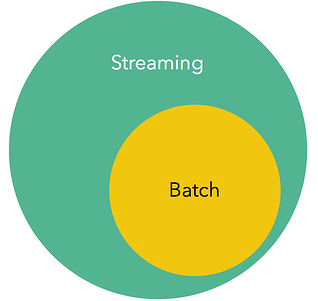
\includegraphics[scale=0.5]{figures/streaming-subset-batch.png}
      \caption{Stream processing as a superset of batch processing}
      \label{fig:stream-superset}
    \end{center}
\end{figure}

\begin{figure}[!htb]
    \begin{center}
      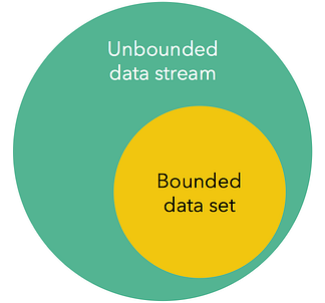
\includegraphics[scale=0.5]{figures/unbounded-superset-bounded.png}
      \caption{Unbounded data streams as a superset of bounded data sets}
      \label{fig:unbounded-bounded-superset}
    \end{center}
\end{figure}


In Section 2.2 we will cover exactly how an unbounded data set (also known as a data stream) can be converted into a bounded data set with the use of windows.

\section{From unbounded streams to finite data sets} \label{sec:windows}

In Section 2.1 we have defined a data stream as an unbounded data set. But what exactly are the issues of working with an infinite stream of data? Why might we need to convert it into a bounded data set and how to do so? In this Section, we will analyze such issues and present sliding windows as the solution.

% boundless aggregations no need for windows
Computations over an unbounded data set are possible. For example, computing the \textit{average} of an event's field for all incoming events is computationally trivial: we need only to store the total number of events (one integer) and the current total sum (one double) of all events arriving to the system. However, is this boundless average over the stream of events useful? While in some scenarios it may be, more often than not we would like to introduce some boundaries into our computations. For instance, consider the monitoring of machines spread out across multiple racks in a large data center and its temperatures. Assume that temperatures measured across all racks are sent to a monitoring system in the form of a data stream. The average temperature of a machine over an infinite period (\textit{i.e.} since the machine was deployed) is of little value for detecting if the equipment is currently overheating, and to trigger the appropriate action to prevent a failure. In this scenario, an average of the temperatures per rack and for the last 5 minutes allows for more actionable context, in this case identifying a likely-to-fail rack. To obtain such insight requires computing the average over the last 5 minutes' worth of data, effectively defining a begin and end --- \textit{i.e.} all the data between the current timestamp in minutes \textit{t} and \textit{t-5}. By creating such a conceptual range, we realize that in practice we need a bounded data set. Partitioning an infinite data stream to obtain such a finite data set is made through the use of windows.

\subsection{Sliding Windows}

Botan et. al \cite{Botan-SECRET} formally define a window as:

\begin{definition}
A window W over a stream S is a finite subset of S"
\end{definition}

% 2 dimensions of windows
Windows can be categorized by two dimensions: the window size $W$ and the sliding step size $S$. Windows can be defined as tuple or time-based. Tuple-based windows are windows whose size is defined by \emph{number} of items contained in the window, whereas time-based windows are windows whose size is defined by the total \emph{time} a window can store. For instance, a tuple-based window of size $10^3$ tuples will store exactly $10^3$ items. In contrast, a time-based window storing the last 5 minutes of events can contain a varying number of tuples but will always keep the events arrived in the last 5 minutes. A window slides over incoming data and groups it, enabling us to compute aggregations over a defined and bounded set of events. The step size \textit{S} of a windowing technique is formally defined as the distance between consecutive windows \cite{Botan-SECRET}. This means that two consecutive windows W\textsubscript{1} and W\textsubscript{2} are exactly \textit{S} units away. As mentioned, these units can be units of time or a number of tuples.

Windows can also be characterized by how they move across data, \textit{i.e.}, how the step $S$ is defined. The three most common ways are: true sliding, stepping or tumbling windows. A true sliding window is a window with an unitary step, i.e., where $S = 1$. At each step, the window advances one unit, which may be one event for tuple-based steps, or one time-unit whether that is in milliseconds, seconds, days, weeks or another magnitude of time, measured based on the system clock or event time. Such a true sliding movement can be observed in Figure \ref{fig:sliding-window} with a tuple-based window of size \textit{W} of three tuples and unitary step. 

\begin{figure}[!htb]
    \begin{center}
      \hspace*{0.6in}
      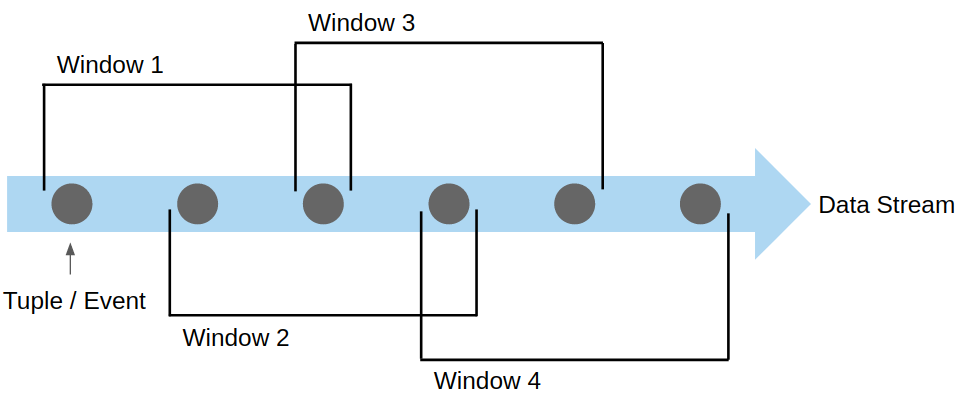
\includegraphics[scale=0.35]{figures/sliding.png}
      \caption[True sliding window]{True sliding window, W=3, S=1}
      \label{fig:sliding-window} 
    \end{center}
\end{figure} 

% stepping windows (per x units over Y window size)
% stepping: step > 1 < window size
A stepping window behaves exactly like a true sliding one but the step size \textit{S} is not unitary, \textit{i.e.}, $S > 1$. In other words, a stepping window is defined by any window size \textit{W} and steps \textit{S} greater than a unit. Figure \ref{fig:stepping-window} represents a stepping tuple-based window of size \textit{W} of three and a stepping size \textit{S} of two.

\textcolor{red}{TODO change all window drawings to a not horrendous style}

\begin{figure}[!htb]
    \begin{center}
      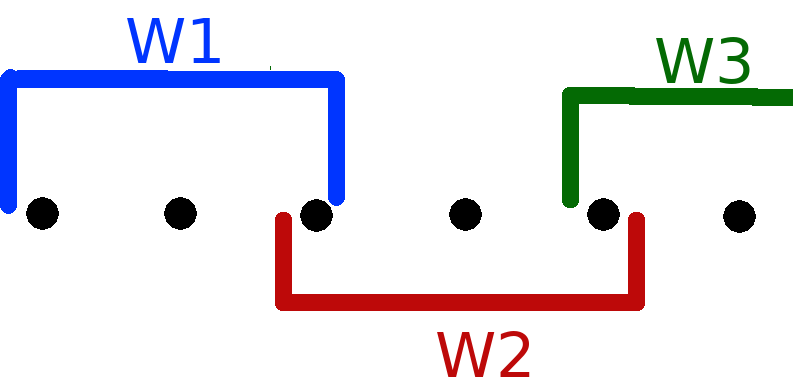
\includegraphics[scale=0.3]{figures/stepping.png}
      \caption[Stepping window]{Stepping window, W=3, S=2}
      \label{fig:stepping-window}
    \end{center}
\end{figure}

% tumbling: step = window size
A tumbling window is a window with a stepping size as large as the window, \textit{i.e.}, $S = W$. Hence, tumbling windows partition the stream into non-overlapping chunks with the same size. Since the intersection of different tumbling windows is always empty, each event is said to belong to exactly one tumbling window. An example of a tumbling window can be seen in Figure \ref{fig:tumbling-window} with a tuple-based window of size \textit{W} of three and an equally large step size \textit{S}.

\begin{figure}[!htb]
    \begin{center}
      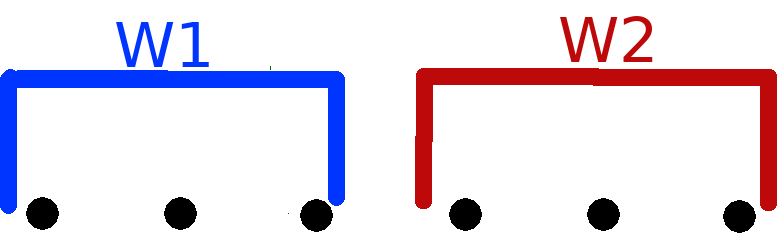
\includegraphics[scale=0.3]{figures/tumbling.png}
      \caption[Tumbling window]{Tumbling window, W=S=3}
      \label{fig:tumbling-window}
    \end{center}
\end{figure}

The mathematical expression below summarizes our categorization of sliding windows.
\begin{equation} 
\label{math:windows}
  Sliding\ window \,\, of \,\, size \,\, W, \,\, step \,\, S =
    \begin{cases}
      true \,\, sliding & \text{if \textit{S}=1}\\
      stepping & \text{if \textit{S}>1}\\
      tumbling & \text{if \textit{S}=\textit{W}}
    \end{cases}
\end{equation}

For the scope of this Thesis, we will work under a tuple-based true sliding window framework. However, despite focusing on tuple-based true sliding windows, our approach is just as valid for time-based windows and other step values as well.

\section{Aggregations over data} \label{sec:aggregations}

An aggregation --- also known as a fold, reduce or accumulate function --- is an operation that reduces a collection of values into a single one. Examples of such are the computation of data set sums, minima, averages or the number of distinct elements (cardinality). An aggregation may be exact or approximate. Exact aggregations compute a value from a sequence of elements, where no error or loss of resolution exists. On the other hand, approximate aggregations have an error margin to the associated aggregation value which is usually controllable by adjusting a set of parameters. 
Approximate aggregations are most useful in situations where memory is limited, the volume of data to process is large and/or computing the exact aggregation can not be done in useful time. Thus, approximate aggregators trade precision of results for efficient time and space usage. In Section \ref{sec:pds} we explore approximate aggregators that make such a trade-off.

Aggregations are present in most programming languages and frameworks. Quoting from the Java programming language documentation on the \textit{Stream.reduce()} method \cite{Java13StreamReduce}: 
\textit{"A reduction operation (also called a fold) takes a sequence of input elements and combines them into a single summary result by repeated application of a combining operation"}. Similarly, the MapReduce \cite{MapReduce} paradigm consists of first applying \textit{map} steps to the collection of data and then a \textit{reduce} one. \textit{Map} tasks will transform each item as desired and the \textit{reduce} task will merge the collection into a single value. Reduce methods make use of a \textit{combine} function and recursively apply it. The \textit{combine} function takes the current aggregation value and combines it with the next item in the set, returning the new aggregated state. Doing this recursively for each item in the collection results in a single value: the aggregate value. The combine function is here on forward represented by $\oplus$ and the identity or neutral element of the aggregation by $\overline{\theta}$.

\subsection{Sliding Window Aggregations}

While some aggregations can be computed on an infinite data set, often we want to compute these over a finite one. As we have seen in Section \ref{sec:windows}, we can obtain a bounded data set from a data stream by applying windowing techniques. When doing so, we obtain a finite data set denoted as a sliding window and compute aggregations over it. Tangwongsan \emph{et. al} define such aggregations over sliding windows as Sliding Window Aggregations (SWAGs) \cite{Tangwongsan-Sliding-Window-Aggregation-Algorithms}. As an example of a SWAG, consider the data center temperature monitoring problem from Section \ref{sec:windows}. In this example, we wanted to compute the average temperature per rack in the data center in the last 5 minutes. If we translate this SWAG into streaming SQL following a similar syntax to the one provided by Apache Flink \cite{ApacheFlink} we would get:

\begin{verbatim}
SELECT rack_id, AVG(temperature)
FROM Temperatures
GROUP BY TUMBLE(timestamp, Time.minutes(5), rack_id)
\end{verbatim}

In the query above, the
\texttt{TUMBLE(timestamp, Time.minutes(5), rack\_id)} statement groups incoming data using time-based tumbling windows of 5 minutes duration, using the \texttt{timestamp} field to evict events not in this time interval. The resulting list of rows has \texttt{rack\_id} as its key and as corresponding value a list of temperatures, from the past 5 minutes. Finally, for each rack and its list of temperatures, we compute an \texttt{AVG} aggregation, resulting in the average temperature per rack in the past 5 minutes. Note that this is very similar to any aggregation made in a standard Database Management System (DBMS). The main difference is that in standard SQL the \texttt{GROUP BY} clause includes only the columns on which the data will be grouped while in streaming SQL the \texttt{GROUP BY} also specifies the type of window used (\textit{e.g.} in this case, a tumbling window).


\subsection{Sliding Window Aggregation Algorithms} \label{sec:back-swag-algs}

A sliding window aggregation algorithm allows the computation of an exact or approximate aggregation over a sliding window. A SWAG algorithm may restrict the set of computable aggregations based on their properties. Different SWAG algorithms use different data structures for the window contents and the incremental aggregation state.

Two of the most basic SWAG algorithms are \textit{Recalculate-From-Scratch (RFS)} and \textit{Subtract-On-Evict (SOE)}. Recalculate-From-Scratch (RFS) is the simplest and most general SWAG algorithm. As the name suggests, this algorithm recomputes the aggregation over the entire window for each update. For instance, the computation of a sum over a sliding window using RFS means that whenever the window changes all elements are summed. This approach works for every aggregation. However, given \textit{n} as the window size, this algorithm takes \textit{O(n)} space and time complexity which makes it unfit in most scenarios of large scale data processing. Recall that the combine function is represented by $\oplus$ and the identity or neutral element of the aggregation by $\overline{\theta}$. Pseudocode for the Recalculate-From-Scratch algorithm is shown in Algorithm \ref{pseudo:rfs}.
  

\begin{algorithm}
    \caption{Recalculate-From-Scratch insert, evict and query methods}
    \label{pseudo:rfs}
    \begin{algorithmic}[1]
        \Function{query}{vals}
            \State $agg\gets\overline{\theta}$
            \ForEach {$v \in vals$}
                \State $agg \gets agg \oplus v$
            \EndFor
            \State \Return $agg$
        \EndFunction
        
        
        \Function{insert}{vals, v}
        
            \State $vals.pushBack(v)$
        \EndFunction
        
        
        \Function{evict}{vals}
        
            \State $vals.popFront()$
        \EndFunction
    \end{algorithmic}
\end{algorithm}

Subtract-On-Evict (SOE) on the other hand, is a SWAG algorithm that incrementally computes the aggregation value. For each element inserted or evicted from the window, the aggregation value is updated without recomputing the entire aggregation like in RFS. SOE relies on expiring the evicted elements from the aggregation state. Hence, SOE only works for \textit{invertible} aggregations, that is, a function $\ominus$ exists such that $(x \oplus y) \ominus y = x$, for all $x$ and $y$. To illustrate the differences between SOE and RFS, consider the computation of a sum aggregation over a sliding window. The total sum of the window will be the aggregation state or value. When inserting an element, the updated total window sum equals the current total sum plus ($\oplus$) the new element. The sum aggregation is considered \textit{invertible} because, when evicting an element, the new aggregation state is the total sum computed thus far minus ($\ominus$) the evicted element. With window size of \textit{n}, SOE has \textit{O(n)} space complexity and \textit{O(1)} time complexity. However, aggregations are not always invertible thus making this algorithm very restrictive and not always applicable. Algorithm \ref{pseudo:soe} shows pseudocode for SOE.

\begin{algorithm}
    \caption{Subtract-On-Evict insert, evict and query methods}
    \label{pseudo:soe}
    \begin{algorithmic}[1]
        \Function{query}{}
        
            \State \Return $agg$
        \EndFunction
        
        
        \Function{insert}{vals, v}
        
            \State $vals.pushBack(v)$
            \State $agg \gets agg \oplus v$
        \EndFunction
        
        
        \Function{evict}{vals}
        
            \State $v \gets vals.popFront()$
            \State $agg \gets agg \ominus val$
        \EndFunction
    \end{algorithmic}
\end{algorithm}

\subsection{Aggregation properties}
\label{sec:agg-properties}

On the previous Section, we presented Subtract-On-Evict as an improvement over Recalculate-From-Scratch based on the idea of aggregation invertibility. The question then becomes if there are other aggregation properties besides invertibility that must be taken into account when analyzing general stream processing algorithms.

As it turns out, besides \textit{invertibility}, other properties allow us to group aggregations in different families. Tangwongsan et al. construct Table \ref{tbl:aggregations-properties} to summarize the aggregation families and satisfying properties \cite{Tangwongsan-Sliding-Window-Aggregation-Algorithms}.

To understand these properties, we must be familiar with the \textit{combine} and \textit{query} functions. The already mentioned \textit{combine} function merges the incoming event with the incrementally computed aggregation state. The \textit{query} function is responsible for returning a result for a given query according to the current aggregation state. For instance, consider once again the use case of computing a sum aggregation over a window of data. The \textit{combine} function would be the arithmetic operator \textit{+} and would merge the current aggregation state --- \textit{i.e.} the current sum value --- with the new incoming event. The \textit{query} function would return the current aggregation state --- \textit{i.e.} return the total sum computed.


Based on the \textit{combine} and \textit{query} functions, the following are formal definitions of these properties. An aggregation is said to have:

\begin{enumerate}
    \item  an \textbf{\textit{invertible combine}} if a function $\ominus$ exists such that $(x \oplus y) \ominus y = x$, for all $x$ and $y$
    
    \item  an \textbf{\textit{associative combine}} if $(x \oplus y) \oplus z = x \oplus (y \oplus z)$, for all $x$ and $y$
    
    \item  a \textbf{\textit{commutative combine}} if $x \oplus y = y \oplus x$, for all $x$ and $y$
    
    \item  a \textbf{\textit{size-preserving combine}} if the aggregation state resulting from $\oplus$ always occupies the same space in memory
   
    \item  a \textbf{\textit{unary query}} if the query does not need any parameters --- \textit{e.g.} a membership test with a Bloom filter would require the element to test membership for as a parameter so it is not unary; returning the total sum is unary since it does not require any parameters
\end{enumerate}

\begin{table}[!htb]
\begin{center}
     \begin{tabular}{p{2cm}|p{1.5cm}p{1.5cm}p{1.5cm}p{1.5cm}p{1.6cm}|}
                 & \rotatebox{35}{\textbf{invertible combine}} & \rotatebox{35}{\textbf{associative combine}} & \rotatebox{35}{\textbf{commutative combine}} & \rotatebox{35}{\textbf{size-preserving combine}} & \rotatebox{35}{\textbf{unary query}}
                 \\
                 \hline
    \textbf{sum-like}     & \checkmark & \checkmark               & \checkmark               & \checkmark                   & \checkmark       \\
    \textbf{collect-like} & \checkmark              & \checkmark               & $\times$               & $\times$                   & ?           \\
    \textbf{median-like}  & \checkmark              & \checkmark               & \checkmark               & $\times$                   & ?           \\
    \textbf{max-like}     & $\times$              & \checkmark               & ?                   & \checkmark                   & \checkmark       \\
    \textbf{sketch-like}  & $\times$              & \checkmark               & \checkmark               & \checkmark                   & $\times$      
    \end{tabular}
    
    \end{center}
    \caption[Aggregation properties]{Aggregation properties. Checkmarks (\checkmark), crosses ($\times$), and question marks (?) indicate a property is true for all, false for all, or false for some of a given group of like operations, respectively}
  \label{tbl:aggregations-properties}
\end{table}

According to these properties, Tangwongsan et al. define five aggregation families \cite{Tangwongsan-Sliding-Window-Aggregation-Algorithms}. These are the sum, collect, median, max and sketch-like families. The sum-like family of aggregations comprises aggregations that have an invertible, associative, commutative and size-preserving \textit{combine} as well as a unary \textit{query} function. Examples of such aggregations are the sum, count, mean/average and standard deviation operations. The collect-like family of aggregations has an invertible and associative \textit{combine} function but their \textit{query} function is not always unary. For example, keeping a string concatenation aggregation is invertible and associative but not commutative nor size-preserving. While in the string concatenation case you do not need to pass any arguments to the \textit{query} function, in the case of another collect-like aggregation, for instance, keeping track of the \textit{i-th} youngest element, you need to specify in your query the parameter \textit{i} (\textit{e.g.} the 5th youngest element). Hence, their \textit{query} function is not always unary. The median-like family of aggregations contains for example the percentile operation. For example, the percentile aggregation is invertible, associative and commutative but not size-preserving and requires an argument to the \textit{query} function: the percentile to compute (\textit{e.g.} percentile 95 or 99). The max-like family comprises aggregations like the maximum or minimum, operations that are not invertible but associative and size-preserving, as well as unary from a \textit{query} function perspective. The final family, the sketch-like family, comprises aggregations that are usually solved by approximate aggregators, also called probabilistic data structures or \textit{sketches}. These aggregations can be membership queries, item frequency estimation or cardinality estimation.

The aggregation properties analyzed in this Section will be used to evaluate SWAG algorithms. Different algorithms might only apply to certain families of aggregations. This way, the multiple SWAG algorithms presented throughout this Thesis will be analyzed not only on their time and space complexity but also on the restrictions they impose regarding the aggregation' properties required. For example, under this framework, to implement Subtract-On-Evict (SOE), both the \textit{combine} $\oplus$ and its inverse $\ominus$ functions must be implemented so that SOE applies $\ominus$ to expire the evicted element from the aggregation state. Since SOE only restriction is for the aggregation to be invertible it works for the \textit{sum-like}, \textit{collect-like} and \textit{median-like} families in Table \ref{tbl:aggregations-properties}.

\section{Exponential Moving Averages} \label{sec:emas}

We talked about sliding window aggregations and algorithms to compute them. We observed that the contents of the sliding window must be stored in memory in order to evict the oldest event and discount its effect from the aggregation when a new one is inserted. In this Section we analyze Exponential Moving Averages (EMAs). EMAs process each event only upon insertion. Since there is no eviction operation to perform, we do not need to store the whole window of data.

Exponential Moving Averages (also known as Exponential Weighted Moving Averages) \cite{EMA-Everett2011} \cite{EMA-Hunter} \cite{EMA-MarcusB} are a type of reduce functions applied to a sequence of elements, one at a time in a orderly fashion, to compute a weighted average, using different weights for each element. These weights decrease exponentially with the age of the observations. In other words, EMAs give higher weights to more recent data points. Figures \ref{fig:window-weights} and \ref{fig:ema-weights} show the weights applied to past events. In a typical sliding window, events either have weight of one (inside the window) or zero (outside the window) whereas EMAs give exponentially smaller weights to older events.

\begin{figure}[!htb]
\centering
\begin{minipage}{.5\textwidth}
  \centering
      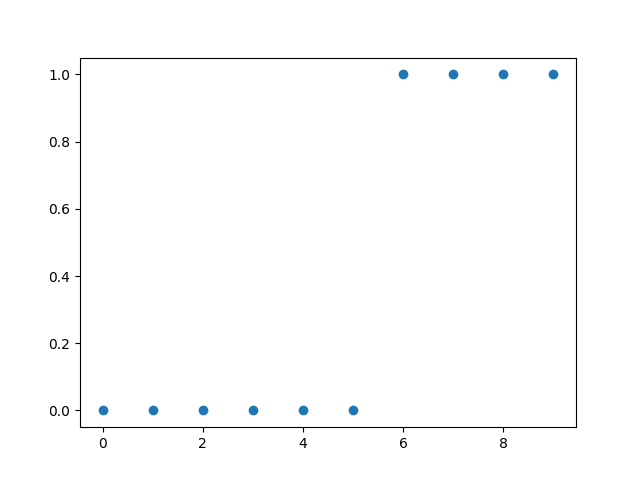
\includegraphics[scale=0.5]{figures/window-weights.png}
  \captionof{figure}{Window weights}
  \label{fig:window-weights}
\end{minipage}%
\begin{minipage}{.5\textwidth}
  \centering
      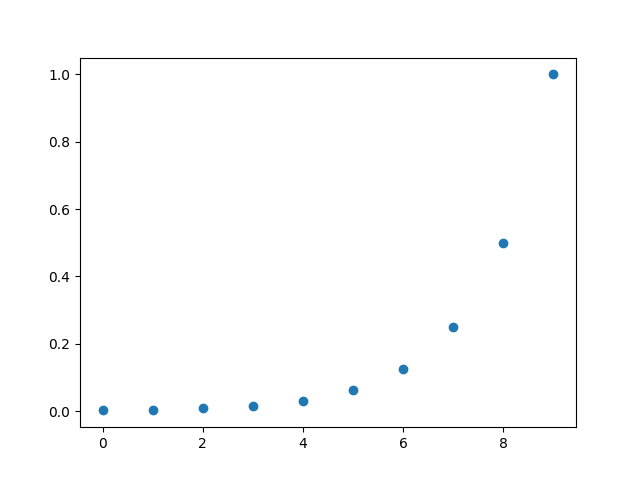
\includegraphics[scale=0.5]{figures/ema-weights.png}
  \captionof{figure}{EMA weights}
  \label{fig:ema-weights}
\end{minipage}
\end{figure}


EMAs are recursive: the EMA value at timestamp \textit{t} depends only on the EMA value at timestamp \textit{t-1}. This recursive property allows us to store only one EMA value and continuously update it for each new value val\textsubscript{t}, based on the following recursion formula:
\begin{definition}
EMA\textsubscript{t} = EMA\textsubscript{t-1} * $2^{-\frac{\delta_t}{\tau_{1/2}}}$ + val\textsubscript{t}
\label{def:ema}
\end{definition}
where $\delta_t$ is the time passed between \textit{t} and \textit{t-1} and $\tau_{1/2}$ is the time-based half-life of the EMA. 

The half-life $\tau_{1/2}$ controls how fast old events are forgotten. The half-life is the amount of time that it takes for an element to see its contribution or weight reduced to half. For instance, with $\tau_{1/2} = 1s$, for each $\delta_t = 1s$ step, we reduce the weights applied to each event by half. 

Note that it is also possible to express a tuple-based half-life $n_{1/2}$, \textit{i.e.}, how many tuples or events must the EMA process before a certain element has its weight reduced by half. In this case, the definition does not take into account the time passed between events:
\begin{definition}
EMA\textsubscript{t} = EMA\textsubscript{t-1} * $2^{-\frac{1}{n_{1/2}}}$ + val\textsubscript{t}
\label{def:tuple-ema}
\end{definition}
For example, with a tuple-based half-life of $\tau = 1$ tuple, for each new tuple all weights are reduced by half.

Definition \ref{def:ema} introduces the recurrence formula for time-based EMAs whereas Definition \ref{def:tuple-ema} works for tuple-based ones. In this Thesis we chose to work with tuple-based EMAs due to its simplicity but our approach can be adjusted to use time-based ones.
\chapter{State of the Art} \label{chap:sota} \minitoc

A data stream has a temporal dimension and the underlying process that generates data can change over time \cite{Aggarwal-Evolving-Data-Streams, Domingos-Mining-Time-Data-Streams}. In this chapter, we discuss the most relevant work for the problem of detecting data pattern shifts in real-time over true sliding windows using resource-lightweight approaches on streaming systems, presented in Chapter \ref{chap:intro}. We present a wide analysis of several categories of algorithms to be able to identify what's the region of this vast landscape of methods that may be useful to build the desired system. 

\section{Outlier Detection in Time-Series Data} \label{sec:outliers}
Blázquez-García \emph{et al.} review state of the art outlier detection techniques and present a taxonomy based on the main aspects of outlier detection methods \cite{Blazquez-Garcia-Review-Anomaly-Detection}. From multiple reviews on these kind of methods \cite{Aggarwal-Outlier-survey, Aguinis-Outlier-survey, Chandola-Outlier-survey-2009, Hodge-Outlier-survey, Xu-outlier-survey-2019} we chose to adopt the taxonomy presented by Blázquez-García \emph{et al.} due to its focus on time-series data.

In this work, the authors define a time-series as a collection of data points sorted by time; and outliers as observations that do not follow the expected behavior. This definition is similar to the concept of outlier provided by Hawkins in 1980 where he states that an outlier is “an observation which deviates so much from other observations as to arouse suspicions that it was
generated by a different mechanism" \cite{Hawkins-Outliers}. Furthermore, Blázquez-García \emph{et al.} allude to the fact that outliers are often referred to in the literature as \textit{"anomalies, discordant observations, discords, exceptions, aberrations, surprises, peculiarities or contaminants"} which for the purpose of their review and this thesis all refer to outliers. In summary, outlier detection refers to the process of finding anomalies in data. An anomaly (or outlier) relates to a point in time where the behavior of the system does not match the expected one. Note that under this definition the presence of outliers or anomalies does not necessarily imply a problem. 

The authors evaluate an outlier detection method on three different axes: the input data type, the outlier type to detect and the uni or multivariate nature of the method. Figure \ref{fig:outlier-taxonomy} presented by the authors in \cite{Blazquez-Garcia-Review-Anomaly-Detection} summarizes these categories.

\begin{figure}[!htb]
  \begin{center}
    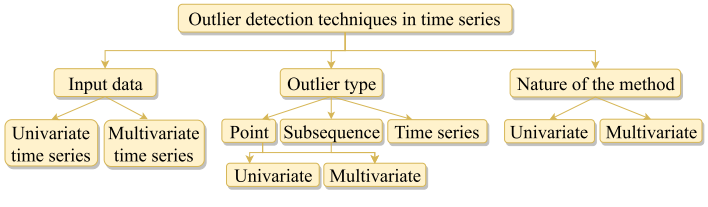
\includegraphics[scale=0.55]{figures/outlier-method-taxonomy.png}
    \caption{Outlier detection method taxonomy}
    \label{fig:outlier-taxonomy}
  \end{center}
\end{figure}

The \textit{input data} axis refers to the type of time-series the method uses as input. According to this criterion, an outlier detection method is said to work with a univariate time-series or a multivariate one. A univariate time-series refers to a time-series consisting of a list of values generated by a single time-dependent variable throughout time. On the other hand, a multivariate time-series has more than one time-dependent variable. Most importantly, each variable is not only time-dependent but may also have dependencies on other variables. 

The \textit{nature of the method} axis refers to the type of analysis performed by the outlier detection method. An outlier detection method may perform a univariate or multivariate analysis. A multivariate analysis considers all variables in the time-series simultaneously while univariate analysis looks at each variable independently. An outlier detection method can take as input a multivariate time-series but perform a univariate analysis, one per time-series of the multivariate input. On the other hand, to perform multivariate analysis, the input data type must be multivariate as well.

The third and final axis is the \textit{outlier type} the method aims to report. The authors identify three distinct outlier types: point outliers, subsequence outliers and time-series outliers. A point outlier corresponds to a single data point in time that deviates from the expected value. These point outliers can be uni or multivariate, depending on the nature of the method. A univariate point outlier is a single time-dependent variable that stands out from the rest of the time-series. On the other hand, a multivariate point outlier takes into account multiple time-dependent variables in comparison to the remaining time-series. Subsequence outliers refer to a sequence of points in time that together show anomalous behavior, but may not be individually considered outliers. Similarly to point outliers, a subsequence outlier may take into account a single time-dependent variable or multiple ones. The authors classify them as univariate subsequence outliers and multivariate subsequence outliers, respectively. Lastly, time-series outliers refer to entire time-series being outliers themselves. This type of outliers can only be detected if the input data is multivariate, to be able to compare multiple time-series.

\subsection{Univariate Point Outlier Detection}

Univariate point outlier detection methods are further broken down into three categories: model-based, density-based and histogram-based (Figure \ref{fig:point-outlier-taxonomy}) .
\begin{figure}[!htb]
  \begin{center}
    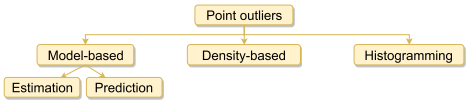
\includegraphics[scale=1]{figures/taxonomy-point-outlier-uni.png}
    \caption[Point outlier detection in univariate time-series taxonomy]{Point outlier detection in univariate time-series taxonomy \cite{Blazquez-Garcia-Review-Anomaly-Detection}}
    \label{fig:point-outlier-taxonomy}
  \end{center}
\end{figure}

The univariate point outlier detection methods based on models are the most common. For each timestamp of the time-series, the models compute the predicted value for the time-dependent variable and compare it with the observed value. If the difference between the predicted value and the observed one is above a certain threshold the data point at the current timestamp is considered an outlier. Mathematically, given the predicted value $p\textsubscript{t}$, the actually observed value $x\textsubscript{t}$ and the user-defined threshold $\alpha$, $x\textsubscript{t}$ is considered an outlier at timestamp \textit{t} if and only if:
\begin{equation*}
    |x\textsubscript{t}-p\textsubscript{t}|>\alpha
\end{equation*}
Model-based point outlier detection methods can be one of two types: estimation or prediction models. The main difference is that estimation model-based methods use past and future data while prediction model-based methods use only past data and infer current and future values. Because of this, prediction model-based outlier detection methods can be used in real-time to process streaming time-series, while estimation based methods can only be used in batch.

Density-based univariate point outlier detection methods rely on the clustering of data points and neighbor counting. For example, nearest neighbor based methods consider a datum an outlier if it has less than $k$ neighbors. Distance between two points is usually measured using the Euclidean distance \cite{elementary-algebra}. Two points are said to be neighbors if they are close to each other --- \textit{i.e.}, the distance between them is less than or equal to a given threshold $\alpha$.

The authors provide little detail on the last category, the histogram-based one. The authors state that these methods are ``based on detecting the points whose removal from the univariate time series results in a histogram representation with lower error than the original''.

\subsubsection{Neighbor-Based Pattern Detection for Windows Over Streaming Data} \label{alg:extran}
 
Yang \emph{et al.} propose \emph{Extra-N} \cite{Yang-Neighbor-Based-Pattern-Detection}, a method for incremental detection of point outliers in sliding window scenarios. Data points are considered outliers if they have few neighbors, \textit{i.e.}, less than a user-defined threshold $\alpha$ of neighbors within a user-defined range $\theta$. Figure \ref{fig:point-outlier} depicts points plotted in their feature space (in this case only two dimensions or features are used, x1 and x2) and a point outlier for $alpha=2$ points and any given $\theta$.
\begin{figure}[!htb]
  \begin{center}
    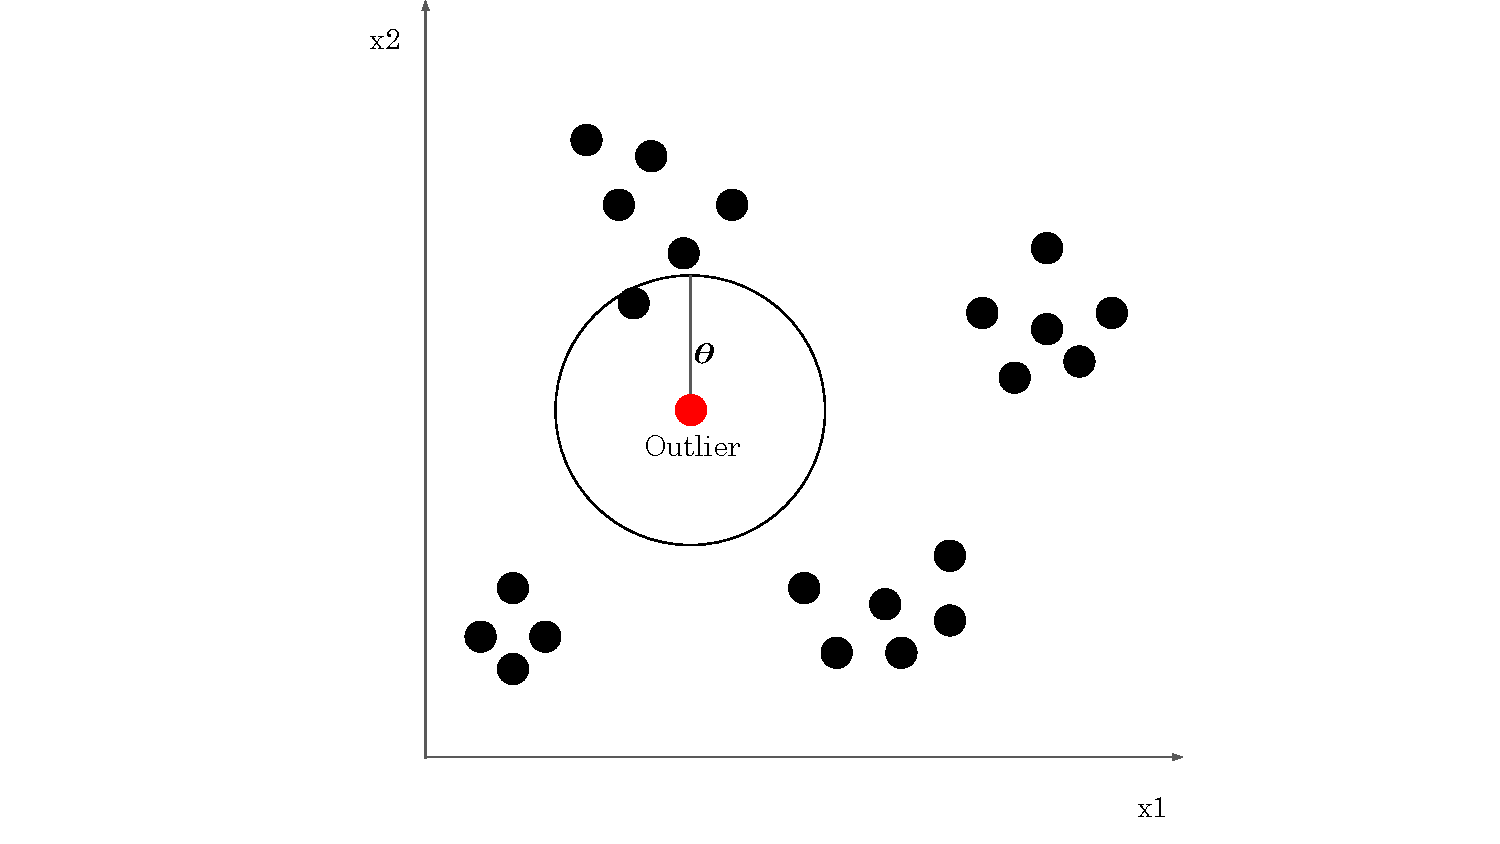
\includegraphics[scale=0.6]{figures/point-outlier.pdf}
    \caption[Density-based point outlier]{Density-based point outlier for $\alpha=2$ and a given $\theta$}
    \label{fig:point-outlier}
  \end{center}
\end{figure}

The key idea is to predict the expiration of any data point in the sliding window and pre-handle the impact it has on its neighbors. The authors introduce the concept of \emph{lifetime neighbor counts} or \textit{lt\_cnt}. The \textit{lt\_cnt} of a data point corresponds to a sequence of predicted neighbor counts, \textit{i.e.}, the number of predicted neighbors a data point has in any future window where it exists. More precisely, each entry on \textit{lt\_cnt} records the number of neighbors that are known to survive in future windows. 

For example, consider a window \textit{W\textsubscript{0}} and a data point \textit{p\textsubscript{0}} with three neighbors: \textit{p\textsubscript{1}}, \textit{p\textsubscript{2}} and \textit{p\textsubscript{3}}. Assume \textit{p\textsubscript{1}} expires after \textit{W\textsubscript{0}}, \textit{p\textsubscript{2}} and \textit{p\textsubscript{3}} expire after \textit{W\textsubscript{1}} and \textit{p\textsubscript{0}} expires after \textit{W\textsubscript{2}}. This implies that at \textit{W\textsubscript{0}}, 
\[ p\textsubscript{0}.lt\_cnt = \{W\textsubscript{0}: 3, W\textsubscript{1}: 2, W\textsubscript{2}: 0\} \]
The lifetime neighbor counts (\textit{lt\_cnt}) carry enough information to compute density-based point outliers: for each data point check if the first or current element of \textit{lt\_cnt} is less than a user-defined threshold $\alpha$ to decide whether that data point is an outlier or not.


\subsubsection*{Method classification}
Extra-N can take both uni or multivariate time-series as input data. However, it does not relate multiple time-series and it does not take into account possible dependencies between different time-dependent variables. In that sense, and according to the presented taxonomy (Figure \ref{fig:outlier-taxonomy}), the method accepts uni or multivariate time-series as input but is of univariate nature. Last but not least, Extra-N aims to detect univariate point outliers. These point outliers are identified based on the density of the region or neighborhood they belong too. Hence, we say Extra-N is a density-based univariate point outlier detection method (Figure \ref{fig:point-outlier-taxonomy}).

\subsubsection*{Time complexity}

To find outliers, Extra-N has to do a linear search through the list of points and check the neighbor counts. Hence, for outlier detection, this method shows \textit{O(n)} complexity with \textit{n} as the number of points. Additionally, for each new data point \textit{p\textsubscript{i}}, Extra-N has to perform a range query search centered on it to find its neighbors and increment their lifetime neighbor counts by one. The runtime complexity of a range query search is \textit{O(log(n))} \cite{range-query-log} with \textit{n} as the number of data points.

In summary, Extra-N shows logarithmic time complexity when updating the sliding window and linear time complexity when looking for outliers, both relative to the window size.


\subsubsection*{Space complexity}
Extra-N has to keep a lifetime neighbor count dictionary-like object for each window data point. For that reason, Extra-N achieves linear memory consumption relative to the number of data points in the window.

\subsubsection*{Applicability to our Hypothesis}
Extra-N memory consumption grows linearly in regards to window size, so it does not fit our desired lightweight system architecture. Furthermore, updating the sliding window should be done in constant time, which is not the case for Extra-N. Hence, we will not use this algorithm.

\subsubsection{Real-Time Stream Anomaly Detection with Hierarchical Temporal Memory}
Ahmad \& Purdy present an anomaly detection technique based on an online algorithm called Hierarchical Temporal Memory (HTM)\footnote{https://github.com/numenta/nupic} \cite{Ahmad-HTM}. HTM has a few properties that are desirable for data stream anomaly detection scenarios. First, it is an unsupervised algorithm that requires no labels. This property comes in handy when monitoring a data stream in real-time, where labels for incoming data will likely be absent. Additionally, HTM adapts to noisy domains. In other words, random variations in the underlying distribution of incoming data that do not persist throughout time will be ignored. Furthermore, HTM detects both spatial and temporal anomalies --- \textit{i.e.}, changes in magnitudes of data or unusual timing for particular patterns, respectively.   

HTM is an online learning algorithm, meaning that it adapts to changing statistics of the underlying data stream. In other words, if there is a sudden abrupt change in the distribution of a specific time-dependent variable, the algorithm will raise an alert. However, if an initial spike that was assumed to be an anomaly becomes frequent, then the algorithm adapts and assimilates this as "a new reality" and stops classifying it as anomalous. Unfortunately, this property is not desirable in our system. Our stream monitoring system must report changes relatively to an initial static configuration (reference or normality period) and should not accept a new distribution as the new standard.

\subsubsection*{Method classification}
Similarly to Extra-N presented in Section \ref{alg:extran}, the Hierarchical Temporal Memory (HTM) algorithm accepts both uni and multivariate time-series as input data but does not perform a multivariate analysis. Hence, we say it accepts both uni and multivariate inputs but is univariate in nature. HTM focuses on finding point outliers, but unlike Extra-N, which is density-based, HTM is a model-based approach. Specifically, HTM is a prediction model-based approach for univariate point outlier detection (Figures \ref{fig:outlier-taxonomy} and \ref{fig:point-outlier-taxonomy}).


\subsubsection*{Applicability to our Hypothesis}
Online learning algorithms that adapt to data pattern shifts and eventually consider them regular patterns are not viable to our goals. We need a monitoring system that alerts data pattern shifts continuously until they match the initial configuration again. Additionally, insights produced by machine learning models are not human-understandable, leaving the user confused about why an anomaly report was made. In conclusion, we do not deem HTM applicable to our solution.


\subsubsection{DeepAnT}
Munir \emph{et al.} present DeepAnT, a deep learning-based approach for the detection of anomalies in time-series data \cite{Munir-DeepAnT}. DeepAnT uses unlabeled data to capture and learn the distribution of the data stream used to forecast the normal behavior of the time-series. This method is unsupervised - \textit{i.e.}, it requires no labels - which is an advantage in a streaming scenario where real-time decisions have to be made before labels are effectively-known. It is capable of detecting point anomalies in time series data with periodic and seasonal characteristics.

DeepAnT employs a Convolutional Neural Network (CNN) as its time-series predictor module. Before monitoring a data stream, the CNN model must be trained. The model can be trained with a small dataset while achieving good generalization capabilities due to the effective parameter sharing of the CNN. Additionally, the dataset used to train the model does not require labels.

\subsubsection*{Method classification}
DeepAnT takes as input a uni or multivariate time-series but is a univariate method by nature --- \textit{i.e.}, it does not find correlations between multiple time-dependent variables. The model used by DeepAnT is a Convolutional Neural Network (CNN), used to make predictions on the future time-series values and measure differences with the actual observed values. Hence, DeepAnT is a prediction model-based univariate point outlier detection method (Figures \ref{fig:outlier-taxonomy} and \ref{fig:point-outlier-taxonomy}).

\subsubsection*{Applicability to our Hypothesis}
Similar to the HTM algorithm presented, DeepAnT adapts to the underlying distribution of the data stream. In other words, if the data patterns shift from the initial configuration but stabilize, DeepAnT will accept it as it is. As mentioned, our goal is to build a monitoring system that alerts data pattern shifts continuously, until they match the initial configuration again.

\subsection{Univariate Subsequence Outlier Detection} \label{sec:uni-sub-out}
Similarly to point outlier detection methods, Blázquez-García \emph{et al.} \cite{Blazquez-Garcia-Review-Anomaly-Detection} split subsequence outlier detection methods into uni and multivariate ones (Figure \ref{fig:outlier-taxonomy}). Furthermore, the authors split univariate subsequence outlier detection methods into five different axes as seen in Figure \ref{fig:subsequence-outlier-taxonomy}.

\begin{figure}[!htb]
  \begin{center}
    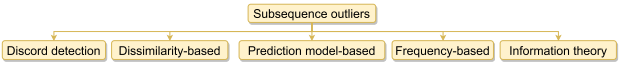
\includegraphics[scale=0.8]{figures/taxonomy-subsequence-outlier-uni.png}
    \caption[Subsequence outlier detection in univariate time-series taxonomy]{Subsequence outlier detection in univariate time-series taxonomy \cite{Blazquez-Garcia-Review-Anomaly-Detection}}
    \label{fig:subsequence-outlier-taxonomy}
  \end{center}
\end{figure}

Methods in the discord detection category compare each subsequence in the time-series with the other subsequences within the time-series to find out the most unusual ones. Each subsequence is compared to the others using a distance metric, for instance, the Euclidean distance. The brute-force way of accomplishing this requires a pairwise comparison of all the subsequences, effectively resulting in quadratic time complexity. These methods find the most unusual subsequence in a time-series. However, as the authors put it, these methods lack a reference or normality state and hence do not accurately report outliers.

On the other hand, univariate subsequence outlier detection methods based on dissimilarity are identical to the previous discord detection based methods but use a reference of normality. The representations used for the subsequences and the reference of normality vary among methods in this class of outlier detection methods but they are based on comparison of the reference or normality subsequence with the ones being analyzed for outlier detection. Once again, the metric used to measure the distance between the reference period subsequence and the other ones depends entirely on the method and subsequence aggregation or representation. Finally, when the measured distance is above a certain threshold, these methods classify the subsequence as an outlier or an anomaly.

Prediction model-based univariate subsequence outlier detection methods assume that the reference or normality period is composed of past events. Similarly to univariate point outlier detection methods based on prediction models, these models train on past data and make predictions of the future. Subsequences that deviate from the model's prediction are classified as outliers.

Frequency-based univariate subsequence outlier detection methods also use a reference period and compute the frequency of each subsequence in the reference or normality period. Hence, a subsequence will be an outlier if it does not appear as frequently as expected in subsequent periods.

Lastly, we have information theory based methods for univariate subsequence outlier detection, which according to the authors \textit{"are closely related to the frequency-based methods"}. This type of method not only measures the frequency of subsequences but relates it with the information carried by the subsequence. Mathematically, a subsequence $S$ will be an outlier if

\begin{equation*}
    I(S) \times F(S) > \alpha
\end{equation*}

with $F(S)$ as the frequency of subsequence $S$, $I(S)$ as the information carried by $S$ and $\alpha$ as a given threshold. According to the authors, \textit{"I(S) is computed taking into account the number of times the symbols within S are repeated through the series"}. The authors explain that if \textit{F(S)} is large --- \textit{i.e.}, S occurs frequently --- then \textit{I(S)} will be closer to 0.

\subsubsection{A two window paradigm algorithm for change detection} \label{kifer}
Kifer \emph{et al.} propose that detecting change in data streams can be reduced to testing if two windows have different underlying distributions \cite{Kifer-Detecting-Change}. The proposed method uses two windows, a reference \textit{W\textsubscript{1}} and a sliding one \textit{W\textsubscript{2}}. Both windows are tuple-based, have size \textit{k} and the sliding window is a true sliding one (recall Section \ref{sec:windows} and the expression \ref{math:windows}). The reference window \textit{W\textsubscript{2}} works as a \textit{reference of normality} and contains the first \textit{k} points of the stream that occurred after the last detected change.

The algorithm begins by filling both windows with the first \textit{k} tuples. Then it slides window \textit{W\textsubscript{2}} by one tuple, since it is a true sliding window, for each incoming event from the data stream. In between slides, the algorithm checks for change by applying a distance function \textit{d} taking as input both the reference and the sliding windows, which measures the discrepancy between both. Whenever this distance is above a certain threshold $\alpha$, the algorithm raises an alert. After raising an alert, both windows are re-initialized with the next \textit{k} items.

Note that after a change is detected, the reference window is updated with the next \textit{k} tuples from the stream. As we have stated, we want a method that does not adapt to the data stream changes and instead keeps raising alerts until the sliding window data distribution returns to the one seen in the reference period. It is trivial to adapt this method to always use the same reference period. To do so, we simply keep the original reference window and do not update it after each alert.

This algorithm reduces change detection in data streams to testing whether two samples --- \textit{reference} and \textit{sliding} windows --- are generated by different distributions. The authors study methods for identifying differences in distribution between two samples and implement them as the \textit{d} function. They provide as examples of a possible \textit{d} function implementation the  Kolmogorov–Smirnov Test \cite{Kolmogorov-Smirnov} and the Wilcoxon-Signed-Rank Test \cite{Wilcoxon}.

\subsubsection*{Method classification}
The method devised by Kifer \emph{et al.} can take uni or multivariate input (if we use one pair of reference/target windows for each time-series) but performs a univariate analysis as it does not find correlations between time-dependent variables. This two-windowed method measures the difference between both windows, the reference and the sliding one. Furthermore, instead of detecting point outliers, the alerts produced indicate the entire window (or subsequence) shows anomalous behavior. Hence, according to the taxonomy presented in Figure \ref{fig:subsequence-outlier-taxonomy}, this method is a dissimilarity-based univariate subsequence outlier detection method.

\subsubsection*{Time complexity}
The authors show that it is possible to compute the distance between both windows in logarithmic time regarding window size \textit{k}. Because the entire sliding window is held in memory, a window update is tantamount to removing the head of the list (element eviction) or appending a new element to the tail (element insertion), which is done in constant time. Thus, for each new event, the method evicts the oldest element, inserts the new one and computes the distance between the reference and sliding windows. In big O notation, the largest and determining factor is the computation of the distance function, done in \textit{O(log(k))} time, with \textit{k} as the size of both windows.

\subsubsection*{Space complexity}
The method makes use of two \textit{k}-sized windows, thus storing \textit{2k} elements. Hence, memory consumption grows linearly with window size.

\subsubsection*{Applicability to our Hypothesis}
In this thesis, we want to detect and alert data pattern shifts with a low memory footprint. The method proposed by Kifer \emph{et al.} grows linearly with window size, making it unfit for large windows, our use case.

However, this two-window paradigm encodes a static normal or reference period in one window and the observed streaming values in a sliding one. Since in this thesis we want to report streaming data pattern shifts relatively to a reference period, we use a similar two-windowed model, but use lightweight and incrementally maintainable aggregations over both windows.


\subsubsection{SAMM: Automatic Model Monitoring for Data Streams} \label{sec:SAMM}

Sampaio \emph{et al.} present SAMM \cite{SAMM}, an automatic model monitoring system for data streams. Similarly to the method presented in Section \ref{kifer}, SAMM uses two windows: the reference window R and the target window T. Window T contains the last $n_t$ elements and window R the $n_r$ elements of a reference period, which is prior to T. SAMM has two main components that interest us: the one responsible for computing the signal and the one that defines the signal threshold. 

The Machine Learning (ML) model being monitored outputs a series of scores for each transaction. The authors build two histograms: one with the model scores for the reference window R and another for the target window T. The signal is a measure of similarity between both histograms $H_R$ and $H_T$. The authors considered using the Kolmogorov-Smirnov \cite{KolomogorovSmirnov, Kolmogorov-Smirnov}, Kuiper \cite{KuiperTest} and Anderson-Darling \cite{AndersonDarling} test but ultimately used the Jensen-Shannon Divergence (JSD) \cite{JSD} to measure the similarity between both histograms. The JSD outputs a value between 0 and 1, with totally different histograms being assigned a value of 1. The signal is then computed by applying the JSD metric to both histograms $H_R$ and $H_T$ at each new event.

To compute the threshold for the JSD signal, the authors maintain a histogram of observed JSD values during streaming. To efficiently maintain the JSD histogram, they devise an algorithm called SPEAR which stands for Streaming Percentiles EstimAtoR. SPEAR is linear in time and space complexity regarding the number of histogram bins, which is a small and fixed constant. This way, for a new JSD value measured between the histogram $H_R$ and histogram $H_T$, they compare it with the histogram and alert if above a certain percentile (\textit{e.g.}, the 99th percentile).

\subsubsection*{Method classification}
SAMM can take uni or multivariate time-series as input but performs a univariate analysis. This method is also a two-windowed method that measures the difference between reference and target sliding windows. The alerts produced report the entire target window as anomalous. According to the taxonomy presented in Figure \ref{fig:subsequence-outlier-taxonomy}, we classify this method as a dissimilarity-based univariate subsequence outlier detection method.

\subsubsection*{Time complexity}
For each new event, SAMM updates the target window T, updates the target histogram $H_T$, computes the JSD between $H_T$ and $H_R$, checks if this value is above a certain percentile and finally updates the histogram of JSDs with the new one. 

Maintaining the target window, \textit{i.e.}, evicting old events and inserting new ones, updating the target histogram $H_T$, computing the JSD between $H_T$ and $H_R$ and checking if it is above a given percentile are all done in constant time. Updating the JSD histogram and dynamically resizing the bins with the SPEAR algorithm takes $O(n)$ time with $n$ as the number of bins. Because the number of bins is small and constant, the update of the JSD histogram is also done in constant time.

Overall, SAMM can process each event in constant time and is suitable for data stream monitoring.

\subsubsection*{Space complexity}
SAMM keeps in memory a reference window, a target window, a reference histogram, a target histogram and a JSD histogram. The histograms can have a small and fixed number of bins so they are not the dominant factor contributing to SAMM's space complexity. Instead, because SAMM keeps two windows in memory, it stores all the events belonging to them. Assuming $n_t$ as the size of target window and $n_r$ as the size of the reference window, SAMM has $O(n_r + n_t)$ space complexity.

\subsubsection*{Applicability to our Hypothesis}
SAMM was designed to work for small-time periods. Hence, for the authors, keeping the reference and target windows in memory was no issue. However, in our solution, we need sublinear time and space complexities to handle large windows of data. This implies we can not directly use SAMM to solve our problem.

However, SAMM has interesting properties we can use in our final solution. First, SAMM also uses a two-window paradigm: a reference and a target sliding one. This is similar to the method seen in Section \ref{kifer}, which may indicate this is a valid and tested approach to follow. Additionally, SAMM aggregates the contents of both windows as histograms and utilizes a statistical divergence test, the Jensen-Shannon Divergence, to measure the similarity (or dissimilarity) between both. This gives them a measure of divergence which they use to raise alerts, which is another great idea to test. Finally, and contrarily to the previous method (Section \ref{kifer}), SAMM does not simply threshold this divergence value: it builds a distribution of divergence values and measures percentiles for new event's divergence values. This allows a user to easier define a threshold: instead of specifying a threshold between 0 and 1 for the JSD value, the user defines only a probability value, \textit{e.g.}, alert when the probability for a JSD value is equal or less than 1\% (percentile 99th).

Even though SAMM is not directly applicable in our context, it provides us with valid and promising ideas to test.


\section{Sliding Window Aggregation Algorithms} \label{sec:sota-swag-algs}

As discussed in Section \ref{sec:back-swag-algs}, a sliding window aggregation algorithm allows the computation of an exact or approximate aggregation over a sliding window. We want to find an aggregation that is suitable to encode our reference and streaming periods so we avoid keeping the entire sliding window in memory. Furthermore, we need an efficient algorithm to incrementally maintain this aggregation. We have presented Recalculate-From-Scratch (RFS) and Subtract-On-Evict (SOE) as the two most basic generic stream processing algorithms. In this section, we analyze other more sophisticated SWAG algorithms that fit different use cases, restraining the set of computable aggregations to certain families, as defined in Table \ref{tbl:aggregations-properties}.

\subsection{Two-Stacks} \label{sec:2stacks}
The Two-Stacks SWAG algorithm works for \textit{associative} aggregations (recall Table \ref{tbl:aggregations-properties}) in scenarios where the sliding window has First-In First-Out (FIFO) semantics --- \textit{i.e.}, elements are evicted in the same order they were inserted. Two-Stacks \cite{Tangwongsan-DABA} implements the FIFO queue using two stacks, namely the front stack F and the back stack B. Each element in each of the stacks is a pair \textit{<val, agg>} where \textit{val} is the item's value and \textit{agg} is the aggregation value of everything below it on the stack. The pseudocode for Two-Stacks can be seen in Algorithm \ref{pseudo:2-stacks}, assuming all functions have access to stacks F and B, with $\oplus$ as the \textit{combine} function and $\overline{\theta}$ as the identity value of the \textit{combine} function, such that $\overline{\theta} \oplus x$ = $x \oplus \overline{\theta}$ = x. For example, if $\oplus$ is the arithmetic sum then $\overline{\theta}$ is 0. If $\oplus$ is the arithmetic multiplication then $\overline{\theta}$ is 1.

Insertion of a new item is always made on stack B. The updated aggregation state is computed using the \textit{combine} function $\oplus$ taking as arguments the aggregation value \textit{agg} of the top element of stack B and the item's value \textit{val}. The pair pushed onto stack B is a pair with \textit{val} and the new aggregation value $\textit{agg} \oplus \textit{val}$.

Evictions correspond to a simple pop from stack F. However, when F is empty, the elements from stack B are flipped onto stack F, re-applying $\oplus$ to make sure each element in F holds the aggregation value of everything below in the stack. Given \textit{n} as the size of stack B, the occasional flip operation takes \textit{O(n)} time.

Computing the sliding window aggregation is done by applying the \textit{combine} function $\oplus$ to the aggregation values of each of the stacks' top element. 

\begin{algorithm}
    \caption[Two-Stacks]{Two-Stacks insert, evict and query methods}
    \label{pseudo:2-stacks}
    \begin{algorithmic}[1]
        \Function{getStackAggregationValue}{stack}
         \If{stack.isEmpty()} 
            \State \Return{$\overline{\theta}$} 
        \Else 
            \State \Return{stack.top().agg} 
        \EndIf
        \EndFunction
        
        \Function{query}{}
            \State \Return{getStackAggregationValue(F) $\oplus$ getStackAggregationValue(B)}
        \EndFunction
        
        
        \Function{insert}{v}
            \State{B.push( \{val: v, agg: getStackAggregationValue(B) $\oplus$ v\} }
        \EndFunction
        
        
        \Function{evict}{}
            \If{F.isEmpty()} \Comment{// Flip B onto F and update top aggregation value}
                \While {\textbf{not} B.isEmpty()}
                    \State{F.push( \{val: B.top().val, agg: B.top().val $\oplus$ getStackAggregationValue(F) \})}
                    \State{B.pop()}
                \EndWhile
            \EndIf
            \State{F.pop()}
        \EndFunction
    \end{algorithmic}
\end{algorithm}

\subsubsection*{Time complexity analysis}
Querying the aggregation state of the window and inserting a new element can be performed in constant time. However, while evicting an item is usually done in constant time, occasionally, a flip operation is required, consuming \textit{O(n)} time, with \textit{n} as the size of stack B. Because this flip is occasionally performed, the time complexity of Two-Stacks is said to be \textit{amortized} constant.

\subsubsection*{Space complexity analysis}
Two-Stacks uses two stacks as auxiliary data structures. The combined size of both stacks is at most the size of the sliding window \textit{n}. Hence, Two-Stacks has linear space complexity \textit{O(n)}.

\subsubsection*{Applicability to our Hypothesis}
Two-Stacks is a general sliding window aggregation algorithm to compute \textit{associative} aggregations. However, it is linear in space and occasionally performs the computationally intensive operation of flipping stack B onto stack F, making it unfit for our use case.


\subsection{De-Amortized Banker’s Aggregator} \label{sec:daba}

The De-Amortized Banker’s Aggregator (DABA) \cite{Tangwongsan-DABA} is a SWAG algorithm that allows the computation of \textit{associative} aggregations. This method carefully handles expensive operations and spreads them along the execution. As a result, the authors are able to turn the average-case behavior into worst-case behavior. This is commonly known as \textit{de-amortization}, hence the name. The main idea behind DABA's design is to avoid occasional expensive operations --- such as the flip operation in Two-Stacks --- by gradually executing them throughout runtime.

\subsection*{Data Structure}

DABA uses two queues, \textit{vals} and \textit{aggs}, both of size \textit{n}, seen in Figure \ref{fig:daba-ds}, which was directly taken from \textit{"Low-Latency Sliding-Window Aggregation in Worst-Case Constant Time"} by Tangwongsan \emph{et al.} Both queues share six pointers --- \textit{F, L, R, A, B} and \textit{E} --- which point to the same position for each queue. These pointers are always ordered as follows: $F \leq L \leq R \leq A \leq B \leq E$.

\begin{figure}[!htb]
    \begin{center}
      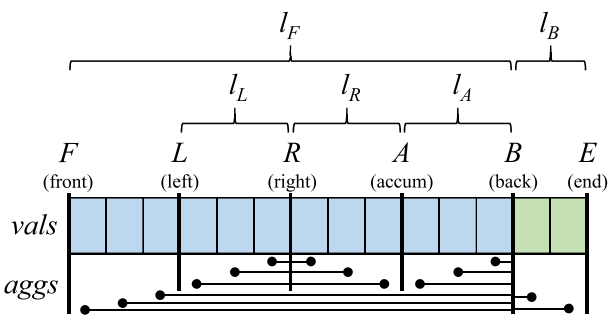
\includegraphics[scale=0.6]{figures/daba-ds.png}
      \caption[DABA data structure]{DABA data structure \cite{Tangwongsan-DABA}}
      \label{fig:daba-ds}
    \end{center}
\end{figure}

Queue \textit{vals} holds the actual sliding window contents. New values are pushed in the back and old values are popped from the front of the queue. Queue \textit{aggs} stores aggregations of sub-ranges of \textit{vals}. Aside from pointer \textit{E}, each pointer defines a sub-list and each sub-list is aggregated either to the left \textbullet--- or to the right ---\textbullet. If a sub-list is aggregated to the left \textbullet---, each \textit{aggs} element will be the aggregation value of all elements in \textit{vals} from that position to the right. On the other hand, if a sub-list is aggregated to the right ---\textbullet, each \textit{aggs} element will be the aggregation value of all elements in \textit{vals} from that position to the left. Values from \textit{vals} can be aggregated to the left or to the right because DABA restricts the aggregation to be \textit{associative} (refer to Table \ref{tbl:aggregations-properties}).

Figure \ref{fig:daba-ds} shows sub-lists \textit{l\textsubscript{F}}, \textit{l\textsubscript{B}}, \textit{l\textsubscript{L}}, \textit{l\textsubscript{R}} and \textit{l\textsubscript{A}}. Sub-list \textit{l\textsubscript{F}} is aggregated to the left for easier eviction. After an element is evicted, the new head of the queue \textit{aggs} --- pointed by \textit{F} --- already contains the aggregation value of all elements from \textit{vals} to its right side. Hence, evicting an element amounts to evicting from both \textit{vals} and \textit{aggs} queue. Similarly, \textit{l\textsubscript{B}} is aggregated to the right to facilitate insertion. Sub-lists \textit{l\textsubscript{L}}, \textit{l\textsubscript{R}} and \textit{l\textsubscript{A}} allow for incremental reversal of the right-aggregated \textit{l\textsubscript{B}} to the left-aggregated \textit{l\textsubscript{F}}. This incremental reversal is tantamount to adjusting pointers that causes shifts in sub-list boundaries. Thus, elements of \textit{aggs} may change from one sub-list to another and need to have its aggregation value recomputed.

Inserting a new element corresponds to pushing a new value \textit{val} in \textit{vals} and pushing the new aggregation value \textit{agg} in \textit{aggs}. The new aggregation value \textit{agg} is computed by applying the \textit{combine} function $\oplus$ to the back element of \textit{aggs} and the new value \textit{val} --- \textit{i.e.}, pushing \textit{val} to \textit{vals} and $\textit{aggs[E]} \oplus \textit{val}$ to \textit{aggs}. 

Evicting old elements is done by evicting the same number of elements from \textit{vals} and \textit{aggs}.

\textit{l\textsubscript{F}} and \textit{l\textsubscript{B}} combined cover the whole \textit{vals} queue --- \textit{i.e.}, every element in the sliding window. \textit{l\textsubscript{F}} is aggregated to the left, thus \textit{aggs[F]} contains the aggregation value of everything in \textit{l\textsubscript{F}}. On the other hand, \textit{l\textsubscript{B}} is aggregated to the right, thus \textit{aggs[E]} stores the aggregation value of everything in \textit{l\textsubscript{B}}. Hence, the aggregation value of the entire window will be the result of \textit{$aggs[F] \oplus aggs[E]$}.


\subsection*{Incremental Reversal of \textit{l\textsubscript{B}} to \textit{l\textsubscript{F}}}

The main conceptual difference between DABA and Two-Stacks is that in Two-Stacks an occasional expensive \textit{flip} operation takes place --- flipping stack B onto stack F --- and in DABA the reversal of \textit{l\textsubscript{B}} to \textit{l\textsubscript{F}} is incremental. This allows DABA to achieve constant time complexity (on average) rather than Two-Stacks' amortized constant time complexity.

Algorithm \ref{pseudo:daba} shows the pseudocode presented by the authors for the DABA algorithm. In reality, after each insertion and eviction, besides the procedure already described, function \textit{fixup} is executed. The \textit{fixup} function performs the incremental reversal of \textit{l\textsubscript{B}} to \textit{l\textsubscript{F}}. Algorithms \ref{pseudo:daba-helpers} and \ref{pseudo:daba} show how such reversal is done but we will not elaborate on such procedure. However, it is important to stress out that this is the core idea of DABA: avoid occasional expensive operations, like Two-Stacks' \textit{flip}, by spreading them out across runtime, in the form of DABA's \textit{fixup}.

\begin{algorithm}
    \caption[De-Amortized Banker’s Aggregator (DABA) helpers]{DABA helper functions}
    \label{pseudo:daba-helpers}
    \begin{algorithmic}[1]
        \Function{getListFAggregationValue}{}
            \If{F == B}
                \State \Return{$\overline{\theta}$}
            \Else
                \State \Return{aggs[F]}
            \EndIf
        \EndFunction
        
        \Function{getListBAggregationValue}{}
            \If{B == E}
                \State \Return{$\overline{\theta}$}
            \Else
                \State \Return{aggs[E - 1]}
            \EndIf
        \EndFunction
        
        \Function{getListLAggregationValue}{}
            \If{L == R}
                \State \Return{$\overline{\theta}$}
            \Else
                \State \Return{aggs[L]}
            \EndIf
        \EndFunction
        
        \Function{getListRAggregationValue}{}
            \If{R == A}
                \State \Return{$\overline{\theta}$}
            \Else
                \State \Return{aggs[A - 1]}
            \EndIf
        \EndFunction
        
        \Function{getListAAggregationValue}{}
            \If{A == B}
                \State \Return{$\overline{\theta}$}
            \Else
                \State \Return{aggs[A]}
            \EndIf
        \EndFunction
        
    \end{algorithmic}
\end{algorithm}

\begin{algorithm}
    \caption[De-Amortized Banker’s Aggregator (DABA)]{DABA insert, evict and query methods}
    \label{pseudo:daba}
    \begin{algorithmic}[1]
        \Function{query}{}
            \State \Return{getListFAggregationValue() $\oplus$ getListBAggregationValue()}
        \EndFunction
        
        \Function{insert}{v}
            \State vals.pushBack(v)
            \State aggs.pushBack(getListBAggregationValue() $\oplus$ v)
            \State fixup()
        \EndFunction
        
        \Function{evict}{}
            \State vals.popFront()
            \State aggs.popFront()
            \State fixup()
        \EndFunction
        
        \Function{fixup}{}
        \If{F == B}
            \State $B \gets E$
            \State $A \gets E$
            \State $R \gets E$
            \State $L \gets E$
        \Else
            \If{L == B}
                \State $L \gets F$
                \State $A \gets E$
                \State $B \gets E$
            \EndIf
            \If{L == R}
                \State $A \gets A + 1$
                \State $R \gets R + 1$
                \State $L \gets L + 1$
            \Else
                \State $aggs[L] \gets getListLAggregationValue() \oplus getListRAggregationValue() \oplus getListAAggregationValue()$
                \State $L \gets L + 1$
                \State $aggs[A - 1] \gets vals[A - 1] \oplus getListAAggregationValue()$
                \State $A \gets A - 1$
            \EndIf
        \EndIf
        \EndFunction
    \end{algorithmic}
\end{algorithm}


\subsection*{Time complexity analysis}
Querying the aggregation state as described is done in constant time. Insertion and eviction of elements take constant time and invoke function \textit{fixup}. The authors develop Theorems that prove function \textit{fixup} is executed in constant time as well. Hence, DABA has constant time complexity.

\subsection*{Space complexity analysis}
DABA stores the window contents in the \textit{vals} queue. Queue \textit{aggs} is of the same size as \textit{vals} and stores partial aggregations over \textit{vals}. Hence, if the window size is \textit{n}, DABA uses two \textit{n}-sized queues. Hence, DABA has \textit{O(n)} space complexity, meaning memory consumption grows linearly with window size.

\subsection*{Applicability to our Hypothesis}
Even though DABA improves on the time complexity of Two-Stacks, it still shows linear space complexity regarding window size. In our monitoring system, we need to analyze large windows of data, thus making DABA inapplicable for our Hypothesis.


\section{Probabilistic Data Structures} \label{sec:pds}
In Section \ref{sec:sota-swag-algs} we presented some state of the art algorithms for computing sliding window aggregations (SWAGs). However, if the aggregation we desire to compute can be approximated, there may exist more memory efficient methods. These aggregators are commonly denoted as sketches or probabilistic data structures and produce results orders-of-magnitude faster than some exact approaches while keeping the memory consumption constant and providing mathematically proven error bounds. Each probabilistic data structure is used for efficient computation of one approximate aggregation, hence we say they are aggregation-specific.

Probabilistic data structures use hash functions to compactly represent a set of items. They require a single pass through the data, which is appropriate for a streaming scenario. Probabilistic data structures have constant space and time complexity \cite{Singh-PDS-BIGD} making them ideal aggregators to build our real-time and low memory footprint system. 

\subsection{Membership Queries and the Bloom Filter} \label{sec:bloom}
% approx aggregation to compute
A Bloom Filter \cite{BLOOM-BLOOMFILTER} approximate aggregator allows membership queries on a set of elements. Bloom Filters answer the query: "Is element \textit{el} in the set of seen elements so far?". Being a probabilistic data structure and approximate aggregator, Bloom Filters' answers have an error associated. \textit{False positive} matches are possible --- \textit{i.e.}, saying \textit{el} is in the set when it is not --- but \textit{false negatives} are not --- \textit{i.e.}, saying \textit{el} is not in the set but it actually is. In other words, a Bloom Filter will accurately identify all items that do not belong in the set but will misclassify some items as being present in the set. Hence, a query returns either \textit{possibly in set} or \textit{definitely not in set}.

% data structures
\subsection*{Data structure}
A Bloom Filter is an array of bits of size \textit{m}, initially all set to 0. Figure \ref{fig:initial-bloom-filter} represents a Bloom Filter with a bit array of size \textit{m}=7 in its initial state.

\begin{figure}[!htb]
    \begin{center}
      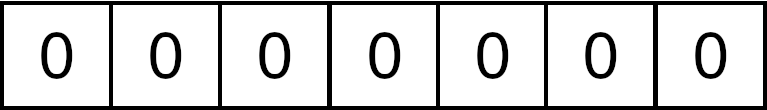
\includegraphics[scale=0.9]{figures/initial-bloom.png}
      \caption[Bloom Filter initial state]{Bloom Filter bit array initial state of \textit{m}=7}
      \label{fig:initial-bloom-filter}
    \end{center}
\end{figure}

% algorithm for insertion
\subsection*{Element Insertion}
Element insertion and query answering make use of \textit{k} hash functions, each mapping elements to a position in the bit array. Adding an element is done by determining which positions should be set to 1. To that end, the new element is fed into each hash function that maps the element to an array position. The resultant \textit{k} outputs are used as the \textit{k} positions of the array to be set to 1. Figure \ref{fig:insertion-bloom-filter} shows the insertion of element \textit{el} in the Bloom Filter, making use of three hash functions (\textit{k}=3), \textit{h\textsubscript{1}}, \textit{h\textsubscript{2}} and \textit{h\textsubscript{3}}. The outputs of the hash functions correspond to the array indexes to set to 1.

\begin{figure}[!htb]
    \begin{center}
      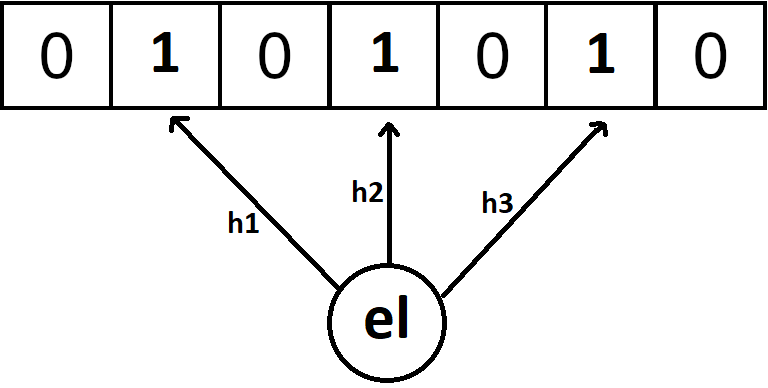
\includegraphics[scale=0.3]{figures/insert-bloom.png}
      \caption[Bloom Filter insertion]{Insertion of element \textit{el} into a Bloom Filter with \textit{m}=7 and \textit{k}=3}
      \label{fig:insertion-bloom-filter}
    \end{center}
\end{figure}

% algorithm for query
\subsection*{Membership Query}
Performing a membership query --- \textit{i.e.}, testing if an element \textit{el} is in the set --- is done by feeding \textit{el} into each one of the \textit{k} hash functions in order to get an array of positions. If \textit{el} was already in the set, all \textit{k} positions should be 1. If any position contains a 0 then the element is \textit{definitely not in set}, as shown in Figure \ref{fig:bloom-filter}. 

\begin{figure}[!htb]
    \begin{center}
      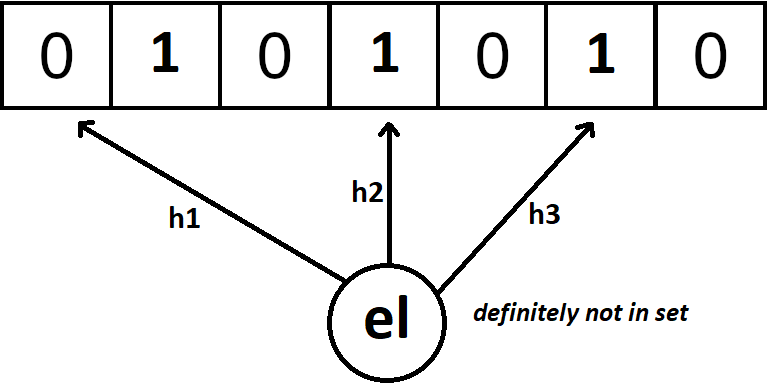
\includegraphics[scale=0.3]{figures/query-bloom.png}
      \caption[Bloom Filter membership query]{Bloom Filter membership test of element \textit{el}. Finding at least one ``0" indicates that it is not in the set.}
      \label{fig:bloom-filter}
    \end{center}
\end{figure}

If all positions are 1 then the element is said to be \textit{possibly in the set}. The reason a Bloom Filter does not provide 100\% certainty that \textit{el} is in the set in case of all positions being 1 is that hash functions may give the same position for two different elements. For example, hash functions \textit{h\textsubscript{1}}, \textit{h\textsubscript{2}} and \textit{h\textsubscript{3}} may map an element \textit{el1} to positions $[1,2,3]$ and an element \textit{el2} to positions $[4,5,6]$. This way, bits in positions $[1,2,3,4,5,6]$ are set to 1. When querying about the membership of a new element \textit{el3}, hash functions \textit{h\textsubscript{1}}, \textit{h\textsubscript{2}} and \textit{h\textsubscript{3}} may map it to positions $[1,3,5]$ as exemplified in Figure \ref{fig:bloom-filter-fp}. Since all of these positions are 1 because of the previous elements inserted, the Bloom Filter returns \textit{"possibly in set"} when in reality \textit{el3} was not in the set. This is considered a \textit{false positive}.

\begin{figure}[!htb]
    \begin{center}
      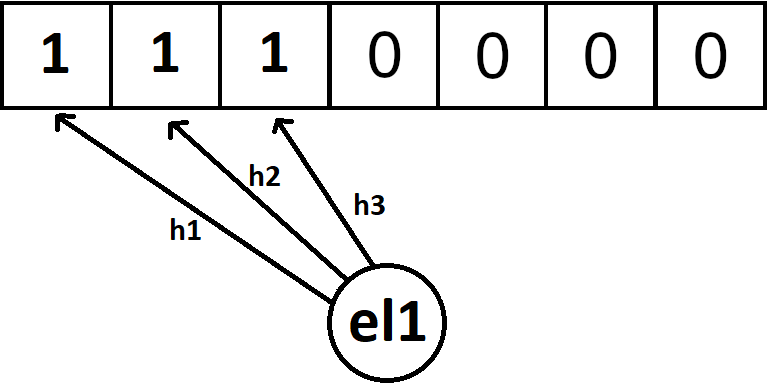
\includegraphics[scale=0.4]{figures/fp-bloom-1.png}
      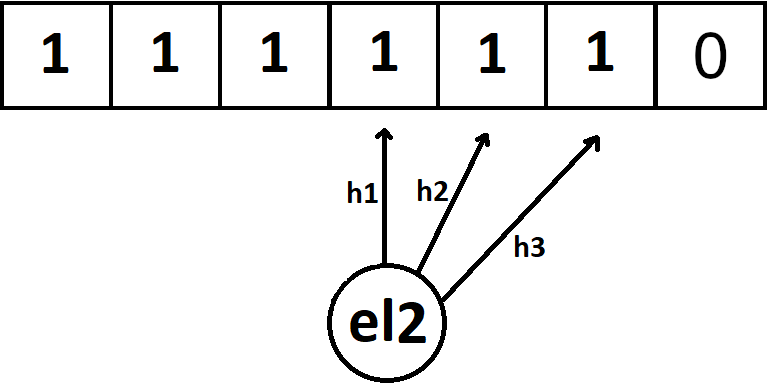
\includegraphics[scale=0.4]{figures/fp-bloom-2.png}
      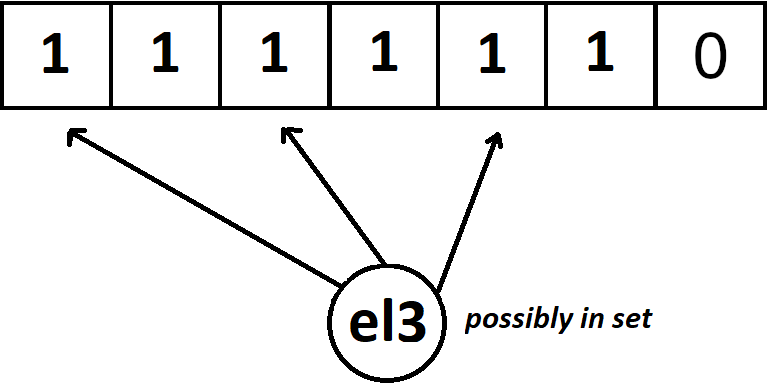
\includegraphics[scale=0.4]{figures/fp-bloom-3.png}
      \caption{Bloom Filter false positive}
      \label{fig:bloom-filter-fp}
    \end{center}
\end{figure}


\subsection*{False Positive rate}
% error bound related with parameters
The false-positive rate is a function of the bit array size \textit{m}, the number of hash functions \textit{k} and the number of elements in the set \textit{n}. It is assumed that the hash functions produce an independent and random index value for each element. 

Mullin presents an analysis of the Bloom Filter in \cite{Mullin-Bloom-Analysis} where he details the false positive rate formula. The probability of one arbitrary bit being set to 1 is:
\begin{equation}
    \frac{1}{m}
\end{equation}
because there are \textit{m} bits. Likewise, the probability of one bit not being set to 1 is
\begin{equation}
    1-\frac{1}{m}
\end{equation}

Mullin states the probability that an arbitrary bit is not set to 1 after one element insertion and corresponding \textit{k} bit updates is:
\begin{equation}
    (1-\frac{1}{m})^\textit{k}
\end{equation}

For \textit{n} insertions, the probability a bit is not set to 1 is:
\begin{equation}
    (1-\frac{1}{m})^\textit{kn}
\end{equation}

Therefore, the probability that an arbitrary bit is set to 1 after \textit{n} insertions is:
\begin{equation}
    1-(1-\frac{1}{m})^\textit{kn}
\end{equation}

Hence, the probability of false positive of a membership query for a new element for \textit{k} hash functions is given by
\begin{equation}
    (1-(1-\frac{1}{m})^\textit{kn})^\textit{k}
\end{equation}

Finally, this false positive rate can be approximated by 
\begin{equation}
    (1-e^\textit{-kn/m})^\textit{k}
\end{equation}


\subsection*{Optimal number of hash functions}
We want to choose the number of hash functions \textit{k} in order to minimize the false positive rate. In order to do so, we must first allocate \textit{m} bits for the Bloom Filter, choosing \textit{m} based on available memory. The value of \textit{k} that minimizes the false positive rate is either of the nearest integers given by:
\begin{equation}
    \frac{m}{n}ln(2)
\end{equation}

\subsection*{Time complexity analysis}
Considering a Bloom Filter with \textit{m} bits and \textit{k} hash functions, insertion has \textit{O(k)} time complexity because all there is to do is run the input through all of the \textit{k} hash functions and set the bits in the given positions to 1. Similarly, query answering has \textit{O(k)} time complexity because it needs only to run the input through the \textit{k} hash functions and check if all bits are set to 1. If so, it returns \textit{possibly in set}. Otherwise it returns \textit{definitely not in set}. 

Note that the time complexity does not at all depend on the number of elements processed by the Bloom Filter and that \textit{k} will be a rather small constant. Hence, the Bloom Filter is said to have constant time complexity.

\subsection*{Space complexity analysis}
Considering a Bloom Filter with \textit{m} bits, the space required is simply the array of \textit{m} bits, thus \textit{O(m)} space complexity. Similarly to the time complexity analysis, we point out that \textit{m} will be constant and that each of the array elements occupies 1 bit. Thus the Bloom Filter has a constant space complexity.

\subsection*{Applicability to our Hypothesis}
Bloom Filters exhibit constant space and time complexity making them possible methods to test our hypothesis. Their false positive rate is tolerable in most scenarios and can be controlled by tweaking the values of \textit{m} and \textit{k}. However, we need to evict old events, and for that reason, Bloom Filters are of no use to us.

\subsection{Item Frequency and the Count-Min Sketch}
% approx aggregation to compute
The Count-Min Sketch (CMS) uses two principles from the discussed Bloom Filters in Section \ref{sec:bloom}. First, Bloom Filters show that precision can be sacrificed to achieve space savings. Second, they are very similar at a technical level.

A Count–Min Sketch \cite{Cormode-CMS} is an approximate aggregator that estimates the frequency of each element in the dataset. It is named after the two basic operations used to provide the estimate: counting (\textit{count}) and computing the minimum (\textit{min}).

% data structures
\subsection*{Data structure}
A CMS is represented by a two-dimensional array (or matrix) with width \textit{w} and depth \textit{d}. A CMS will make use of \textit{d} hash functions, each associated with one row of the matrix. Each hash function will map elements to a position between 1 and \textit{w}, the column of the two-dimensional array. Initially, all of the matrix positions are 0. Figure \ref{fig:initial-cms} represents the two-dimensional array used by the CMS and corresponding dimensions in its initial state. 

\begin{figure}[!htb]
    \begin{center}
      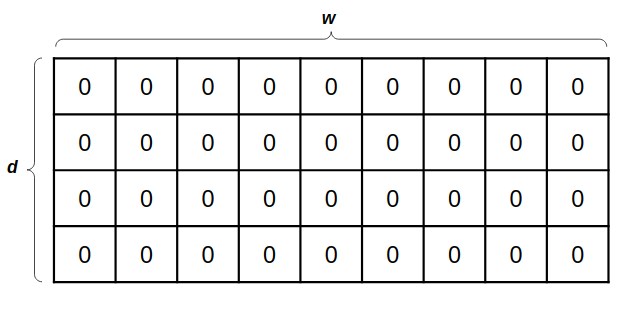
\includegraphics[scale=0.5]{figures/initial-cms.png}
      \caption[Count-Min Sketch initial state]{Count-Min Sketch matrix initial state of \textit{d}=4 and \textit{w}=9}
      \label{fig:initial-cms}
    \end{center}
\end{figure}

% algorithm for insertion
\subsection*{Element Insertion}
When adding an element, for each row \textit{i} of the \textit{d} rows in the matrix, we hash the element using that row's hash function to obtain the result $j$. Lastly, for all obtained pairs of \textit{i} and \textit{j}, increment matrix cells \textit{(i, j)} value by 1, as seen in Figure \ref{fig:cms}. If elements have different weights these can be added instead of incrementing one unit.

\begin{figure}[!htb]
    \begin{center}
      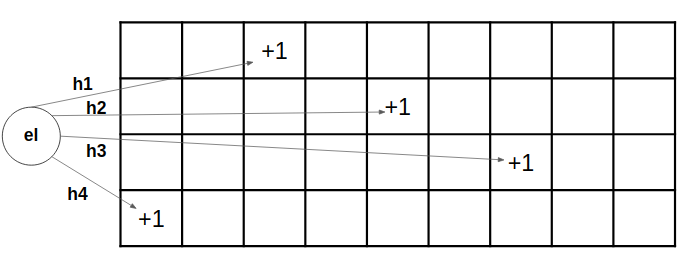
\includegraphics[scale=0.5]{figures/insertion-cms.png}
      \caption[Count-Min Sketch insertion]{CMS mapping element \textit{el} using \textit{d}=4 hash functions to determine the column position for each row and increment it.}
      \label{fig:cms}
    \end{center}
\end{figure}

% algorithm for query
\subsection*{Frequency Query}
Retrieving the minimum frequency of an element \textit{el} can be done by taking the minimum value of all row counts for \textit{el}. Mathematically, the frequency estimate is the minimum value of the set of all row values, for each row \textit{i} of the total \textit{d} rows, given by:
\[ min \{matrix[i][\textit{h\textsubscript{i}}(el)]\} \]

Figure \ref{fig:query-cms} illustrates this procedure, where the result of the query "What is the frequency of \textit{el}?" returns "2".
   
\begin{figure}[!htb]
    \begin{center}
      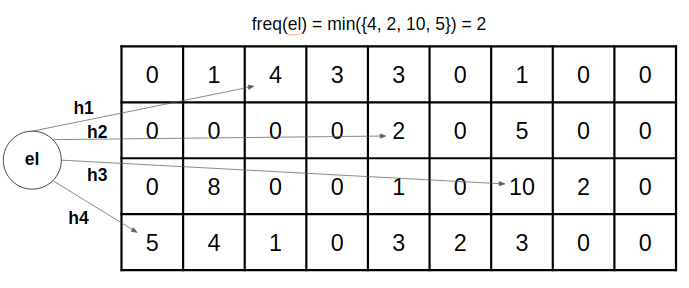
\includegraphics[scale=0.5]{figures/query-cms.png}
      \caption[Count-Min Sketch frequency query]{Count-Min Sketch frequency query of element \textit{el}}
      \label{fig:query-cms}
    \end{center}
\end{figure}

% error bound related with parameters
\subsection*{Optimal number of hash functions} 
For an element \textit{el}, each row will have one position incremented by \textit{el}'s true frequency. However, multiple elements may be mapped to the same position within a row, thus overlapping their frequencies. Hence, for an element \textit{el}, the CMS provides a frequency estimate that is greater or equal to the true frequency of \textit{el} in the set.

The number of hash functions \textit{d} to be used depends on the desired error probability. To achieve an error probability $\delta$, \textit{d} is given by the following expression:
\begin{equation}
    d = \lceil ln \frac{1}{\delta} \rceil
\end{equation}
For example, to achieve an error $\delta$ = 1\%, \textit{d} = 5 hash functions are necessary.

\subsection*{Time complexity analysis}
When adding an element, the Count-Min Sketch loops through each row and applies a constant in time hash function, updating the value of the target cell. Hence, insertion loops through \textit{d} rows and has time complexity of \textit{O(d)}. Similarly, querying the frequency of an element \textit{el} consists of computing the minimum of all row values. Since both insertion and query have constant time complexity, the CMS is constant in time.

\subsection*{Space complexity analysis}
The Count-Min Sketch relies on a two-dimensional matrix as its only data structure. The memory used will correspond to the \textit{wd} counts, hence \textit{O(wd)} space complexity. Since both \textit{w} and \textit{d} are constants, the CMS has constant space complexity.

\subsection*{Applicability to our Hypothesis}
Count-Min Sketches are constant in both time and space. Similarly to Bloom Filters, this makes them ideal candidates for our solution. 

\subsection{Cardinality Estimation and the HyperLogLog} \label{sec:hyper-log-log}

A set of probabilistic counting algorithms is introduced by Flajolet \emph{et al.} in \cite{Flajolet-PCA} to estimate the number of distinct elements of a set --- also known as the cardinality of the set. These techniques are based on \textit{"bit-pattern observables"} in the binary representation of the hashed values. Bit-pattern observables are defined by the authors as \textit{"patterns of bits occurring at the beginning of the (binary) S-values"}, with \textit{S} as the target set.

Later on, the authors propose the LogLog algorithm \cite{Flajolet-LogLog}. In LogLog, the bit-pattern observable recorded for each item is the position of the leftmost 1-bit, denoted as \textit{P}. The authors claim it is related to the total number of distinct elements in the dataset in that it is \textit{"more or less a likely indication that the cardinality of S is at least $2^P$"}.


\subsection*{HyperLogLog}
A couple of years later, the same authors propose HyperLogLog (HLL) \cite{Flajolet-HLL}, an approximate aggregator to compute the cardinality of a set. 

HLL uses the same bit-pattern observable as LogLog --- \textit{P}, the position of the leftmost 1-bit. With LogLog, the authors realize that storing only one observation produces extremely inaccurate predictions due to the high variability of a single value. The proposed solution is to apply \textit{stochastic averaging}. As the authors state, stochastic averaging \textit{"consists in emulating the effect of m experiments"}. Effectively speaking, the authors propose dividing the input stream into \textit{m} substreams or buckets, maintaining one observable per bucket and computing \textit{P} as an average of all bucket values (stochastic averaging).

\subsection*{Data Structure}
HyperLogLog (HLL) maintains \textit{m} bit-pattern observables, each being the leftmost 1-bit position, \textit{P}. Since each position is a single integer, HLL maintains \textit{m} integer counters, as seen in Figure \ref{fig:hll-ds}. Each of these counters holds the maximum value for the bit-pattern observable seen so far. The first bit is assumed to be in position "1" and all counters begin with "0".

\begin{figure}[!htb]
    \begin{center}
       \hspace{0.5in}
      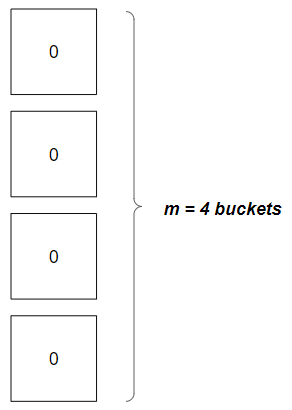
\includegraphics[scale=0.6]{figures/hll-ds.png}
      \caption[HyperLogLog initial state]{HyperLogLog with \textit{m}=4 observable buckets}
      \label{fig:hll-ds}
    \end{center}
\end{figure}


\subsection*{Element Insertion}
In HyperLogLog, new elements are hashed into a binary string. The first \textit{n} bits of the hashed representation will map to one of the $m=2^n$ buckets. Effectively speaking, the first \textit{n} bits work as a \textit{bucket ID}. The bit-pattern observable \textit{P} --- the position of the leftmost 1-bit --- is counted from the binary string discarding the first \textit{n} bits. The observable \textit{P} is stored in the pre-determined bucket if it is greater than the value the bucket contains. 

Figure \ref{fig:hll-insert} demonstrates such procedure for a new element \textit{el}. The hash representation of \textit{el}, using $n=2$ bits, maps to bucket \textit{10}. Discarding the first $n=2$ bits and counting from 1, the position of the leftmost 1-bit is $P=4$. The previous value of bucket \textit{10} was 0 and because $P=4$ is greater than 0 the bucket value is updated.


\begin{figure}[!htb]
    \begin{center}
      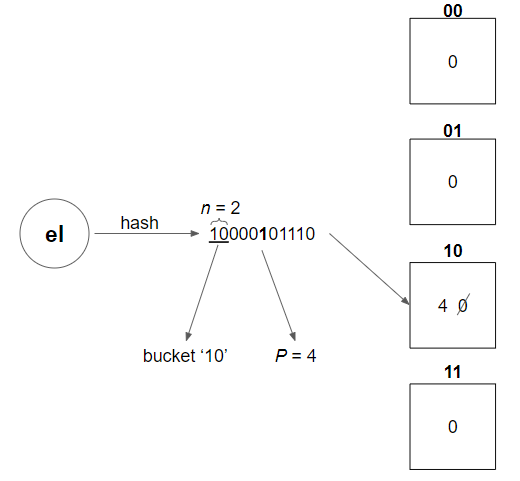
\includegraphics[scale=0.8]{figures/hll-insertion.png}
      \caption[HyperLogLog insertion]{HyperLogLog \textit{el} insertion with \textit{m}=4 and \textit{n}=2 bits}
      \label{fig:hll-insert}
    \end{center}
\end{figure}

\subsection*{Cardinality Query}
The cardinality of the set is estimated to be $2^\textit{P}$ where the bit-pattern observable \textit{P} is the position of the leftmost 1-bit. As discussed, HyperLogLog (HLL) differentiates from LogLog in that it applies a stochastic averaging process. Hence, the value of \textit{P} will be the harmonic mean of all \textit{m} buckets.


\subsection*{Time complexity analysis}
Adding an item is tantamount to hashing it, determining the corresponding bucket based on the first \textit{n} bits, counting the leftmost 1-bit position and updating the bucket value if need be. Estimating the cardinality of the set amounts to finding the maximum value \textit{P} between all buckets and computing $2^P$. Hence, both inserting a new element and estimating the cardinality of the set take constant time.

\subsection*{Space complexity analysis}
Quoting Flajolet \emph{et al.} about the memory consumption and error in the approximations obtained in their experiments in the original HyperLogLog paper \cite{Flajolet-HLL}: 
\say{cardinalities till values over N = $10^9$ can be estimated with a typical accuracy of 2\% using 1.5kB (kilobyte) of storage.}

HyperLogLog uses \textit{m} buckets that store a single integer value, thus the space complexity is \textit{O(m)} where \textit{m} is a rather small constant. Hence, HyperLogLog has constant space complexity.

\subsection*{Applicability to our Hypothesis}
Similar to the previously studied approximate aggregators, HyperLogLog (HLL) has constant space and time complexity and provides an estimate of a set's cardinality. Hence, HLLs are considered valuable aggregators for our thesis.

\section{Sliding Window Aggregations with Probabilistic Data Structures} \label{sec:sliding-pds}
In Section \ref{sec:pds} we presented a set of probabilistic data structures constant in time and space. These structures aggregate an endless stream of data. However, when working with sliding windows there is the need not only to insert new events but to evict old ones. The probabilistic data structures described until now can aggregate new incoming data but do not address the type of temporality needed for sliding windows --- \textit{i.e.}, the ability to expire old elements from the aggregated state.

The probabilistic data structures studied can be implemented under generic sliding window aggregation algorithms like Recalculate-From-Scratch or DABA. However, doing so means we lose the main advantage of using these approximate aggregators: the constant space complexity. For example, cardinality estimation of a sliding window can be done employing the HyperLogLog heuristic of estimating cardinality as $2^\textit{p}$, with \textit{p} as the maximum position seen for the leftmost 1-bit, using DABA \ref{sec:daba} for the computation of \textit{p} per sliding window. With this approach, despite computing the aggregation state in constant time, we have a linear in window size space complexity solution. Thus, in this section, we explore sliding window implementations of the previously discussed probabilistic data structures that keep the space and time complexity at the very least logarithmic.

%\subsection{Sliding Bloom Filter}
%\subsection*{Data Structure}
%\subsection*{Element Insertion}
%\subsection*{Element Eviction}
%\subsection*{Time complexity analysis}
%\subsection*{Space complexity analysis}
%\subsection*{Applicability to our Hypothesis}

%\subsection{Sliding Count-Min Sketch}
%\subsection*{Data Structure}
%\subsection*{Element Insertion}
%\subsection*{Element Eviction}
%\subsection*{Time complexity analysis}
%\subsection*{Space complexity analysis}
%\subsection*{Applicability to our Hypothesis}


\subsection{Sliding HyperLogLog}

The HyperLogLog (HLL) aggregator presented in Section \ref{sec:hyper-log-log} will only be useful to us if it can be implemented efficiently in a sliding window fashion. The HLL aggregator estimates the set's cardinality assuming it is close to $2^\textit{p}$, where \textit{p} is the maximum position seen for the leftmost 1-bit in the binary values of all of the set items' hashes. In practice, all the aggregator has to compute is \textit{p}, the maximum value of all observables. Stochastic averaging is applied by emulating the effects of \textit{m} experiments using \textit{m} buckets to store \textit{m} bit-pattern observables. 


\subsubsection{Sliding HyperLogLog using Lists of Future Possible Maxima} \label{sec:hll-lfpm}

The work of Chabchoub \emph{et al.} adapts the original HLL aggregator from Flajolet \emph{et al.} to work under a sliding window framework  \cite{Chabchoub-Sliding-HLL}.
The main idea behind this implementation is to replace every HLL counter with a \textit{List of Future Possible Maxima (LFPM)}.

\subsubsection*{Data Structure}

The adaptation of the original HLL to work under a sliding window scenario requires the storage of additional information. The original HLL maintained \textit{m} integer counters, each storing the maximum for the leftmost 1-bit position of the analyzed binary strings.  The counter held the maximum value for all the seen binary strings so far but there was no way to expire old items. To allow eviction, the proposed data structure is very similar to the original \textit{m} integer counters but keeps a list of values per bucket and associates a timestamp to each. 

The stochastic averaging process of HLL remains unchanged: incoming items are hashed and distributed across \textit{m} buckets. However, the authors propose keeping a short list of \textit{packets} per bucket instead of a single integer count. A \textit{packet} is defined as a pair <\textit{t\textsubscript{i}, p\textsubscript{i}}> where \textit{t\textsubscript{i}} is the arrival timestamp of the packet and \textit{p\textsubscript{i}} the position of the leftmost 1-bit in the binary hash representation of the associated value. Packets are only kept in the list if they are possible maxima over future windows. Because of that, the authors name this list a ``List of Future Possible Maxima (LFPM)''.

\subsubsection*{Element Insertion \& Eviction}
Similarly to the original HLL, incoming elements are hashed and the first \textit{n} bits of the string are used to map the new element to one of the \textit{m} buckets. The first \textit{n} bits are then discarded and the bit-pattern observable \textit{p} is computed from the remaining string. 

Since each bucket now holds a LFPM instead of a single integer, the procedure for bucket update is different. Upon insertion of an element \textit{k}, a packet $<t_k, p_k>$ is created with t\textsubscript{k} as the timestamp of arrival of the new element \textit{k} and p\textsubscript{k} as the position of the leftmost 1-bit position of \textit{k}'s binary representation. Given the new packet <t\textsubscript{k}, p\textsubscript{k}>, the authors propose the following LFPM update method, that checks for and evicts old packets at each insertion:

\begin{itemize}
    \item Delete \textit{old packets}: packets that do not belong in the window anymore --- \textit{i.e.}, packets <t\textsubscript{i}, p\textsubscript{i}> with t\textsubscript{i} $\leq$ t\textsubscript{k} - WindowSize 
    
    \item Delete less or equally valued packets: packets that will never be a maximum --- \textit{i.e.}, packets <t\textsubscript{i}, p\textsubscript{i}> with p\textsubscript{i} $\leq$ p\textsubscript{k}
    
    \item Add the new packet <t\textsubscript{k}, p\textsubscript{k}>
\end{itemize}


\subsubsection*{Sliding Window Cardinality Query} 

Estimation of cardinality is done similarly to the original HLL cardinality estimation algorithm. To estimate the cardinality at a timestamp \textit{t}, from all \textit{m} buckets and all \textit{m} lists, select packets that are in the window --- \textit{i.e.}, packets <t\textsubscript{i}, p\textsubscript{i}> where t\textsubscript{i} > \textit{t} - WindowSize. This filtering is necessary since the proposed algorithm evicts old packets only at element insertion and at the time of the query some packets may no longer belong to the window. Next, from the filtered set of packets, for each bucket and its list, compute the maximum p\textsubscript{i} value. In the end, compute the harmonic mean between all values, just like the original HLL. The result will be the averaged bit-pattern observable value \textit{p} and the cardinality is estimated to be $2^\textit{p}$.

\subsubsection*{Time complexity analysis}
When performing insertions or evictions, the algorithm requires scanning through the Lists of Future Possible Maxima (LFPMs) to delete old packets or packets that will never be window maxima. Similarly, we need to scan the lists when estimating the cardinality to filter for packets within our window. Denote \textit{L\textsubscript{n}} as the mean size in packets for each LFPM. There are \textit{m} buckets, each with a list. To scan through all lists we need to analyze \textit{m L\textsubscript{n}} elements. 

The authors prove that \textit{L\textsubscript{n}} has an upper bound of \textit{ln(n/m)}, with \textit{n} as the cardinality of the set and \textit{m} as the number of buckets used. Hence, in the worst-case scenario, we need to analyze \textit{m ln(n/m)} elements. This means that a Sliding HLL implementation using Lists of Future Possible Maxima has \textit{O(ln(n))} time complexity, given the number of buckets \textit{m} is constant.

\subsubsection*{Space complexity analysis}
The memory used in the Sliding HLL aggregator implemented with Lists of Future Possible Maxima (LFPMs) amounts to the total size of the \textit{m} lists. Assuming 4 byte timestamps and 1 byte bit-pattern observables for each packet, the aggregator uses \textit{(4+1) L\textsubscript{n} m} bytes. 

The lists are dynamic thus they shrink and grow at runtime. However, \textit{ln(n/m)} was proved to be an upper bound for \textit{L\textsubscript{n}}. Hence, this sliding implementation of the HLL aggregator consumes up to \textit{(4+1) ln(n/m) m} bytes of memory. Considering that the number of buckets \textit{m} is constant, the space complexity of a Sliding HLL implementation with LFPM is \textit{O(ln(n))}.

The authors claim that the proposed sliding version remains as accurate as of the original HLL aggregator. With an additional memory of only 35kB, it is possible to estimate the number of distinct elements in the set with a standard error of 3\% in the presence of up to a million distinct elements.

\subsubsection*{Applicability to our Hypothesis}
Implementing a Sliding HLL using Lists of Future Possible Maxima (LFPMs) shows logarithmic time and space complexity while providing estimates with the same accuracy as the original HLL approximate aggregator. However, the memory consumption is dynamic due to the variable size of the lists. 

Despite the fact memory consumption dynamically changes during runtime, this is a valid approach to test our Hypothesis due to the worst-case scenario being a logarithmic space complexity. However, in Section \ref{sec:hll-drv} we analyze an implementation that is not dynamic in memory during runtime making it a preferred approach.


\subsubsection{Sliding HyperLogLog using Distance Recorder Vectors} \label{sec:hll-drv}

In Section \ref{sec:hll-lfpm} we have analyzed a Sliding HLL implementation where each of the \textit{m} buckets holds a list of values (LFPM) instead of a single integer count. However, the LFPM structure is dynamic and its size varies at runtime. 

The approach proposed by Xu uses a smaller amount of memory that does not change at runtime \cite{Xu-hll-sliding-drv}. The author proposes a special counter: a \textit{Distance Recorder Vector (DRV)}. 

\subsubsection*{Data Structure}
Much like the original HLL and the LFPM Sliding implementation, the Distance Recorder Vector (DRV) approach uses \textit{m} buckets. However, instead of integer counts or lists, each of the buckets stores a DRV. 

A DRV is composed by \textit{$\lceil ln(n/m) \rceil$} records, with \textit{n} as the cardinality of the set. Notice that \textit{n/m} is the average number of distinct elements each bucket \textit{m} is expected to process and that a binary string of size \textit{$\lceil ln(n/m) \rceil$} can represent \textit{n/m} distinct elements. Also recall that the bit-pattern observable \textit{p} used by the HLL is the position of the leftmost 1-bit. In a binary string of size \textit{$\lceil ln(n/m) \rceil$}, \textit{p} will range from 1 to \textit{$\lceil ln(n/m) \rceil$}. The DRV is indexed exactly this way, from 1 to \textit{$\lceil ln(n/m) \rceil$}, and each bit-pattern observable \textit{p} will be used as an index in this vector of records. Essentially, each \textit{p} will have an associated record in a DRV of a bucket.

Initially, all records in the DRV will be set to be infinity or a very large number.

\subsubsection*{Element Insertion}
When an element is inserted, the same procedure as in the original HLL is followed: the element is hashed and \textit{p} is computed from the hashed binary representation. Let us denote the bit-pattern observable of the new element as \textit{p\textsubscript{new}}. For the DRV of that bucket, we increment the value of all records by one. Next, we set position \textit{p\textsubscript{new}} in the DRV to 0 --- \textit{i.e.}, $\textrm{DRV}[p_{new}] = 0$.


\subsubsection*{Sliding Window Cardinality Query} 
This method does not perform element eviction. Instead, the query algorithm assumes that some records in DVR's entries might be expired. 

To estimate the sliding window cardinality is to find the value \textit{p}. To find the value \textit{p} for a bucket, we scan the DRV of that bucket backward. For that, we start at the last element --- positioned at \textit{$\lceil ln(n/m) \rceil$} --- and scan towards the head of the vector. For each record, we check if it is active in the current window. To do so, we check if its value is less than the size of the window. If it is, the record is active. Otherwise, the record is inactive.

If the record is inactive we continue scanning backward. If the record is active, then the position or index currently being scanned is the value of \textit{p} for that bucket. If all records are inactive, the bit-pattern observable \textit{p} is 0.

Stochastic averaging is done just like in the original HLL: compute the harmonic mean of all \textit{p\textsubscript{m}} values from all \textit{m} buckets. The cardinality of the sliding window is then estimated to be $2^\textit{p}$.

\subsubsection*{Time complexity analysis}
When inserting an element, determining its bucket, hashing the element and computing \textit{p} is done in constant time. However, all the  \textit{$\lceil ln(n/m) \rceil$} records must have their value increased by one and this means iterating over the DRV. Setting the element of the DRV indexed by \textit{p} to 0 is done in constant time as well. 

Estimating cardinality is done by scanning the DRV backward until an active record is found. In the worst-case scenario, this means scanning all \textit{$\lceil ln(n/m) \rceil$} records.

Both inserting an element and estimating sliding window cardinality require a scan through \textit{$\lceil ln(n/m) \rceil$} records. This gives us a time complexity of \textit{O(\textit{ln(n)})}, if the number of buckets \textit{m} is constant. 

\subsubsection*{Space complexity analysis}
This approach still uses \textit{m} buckets but each one contains a Distance Recorder Vector (DRV). A DRV is a vector of \textit{$\lceil ln(n/m) \rceil$} elements. Hence, \textit{$m \lceil ln(n/m) \rceil$} elements must be kept in memory, giving us a space complexity of \textit{O(ln(n))} with \textit{n} as the cardinality of the set.

\subsubsection*{Applicability to our Hypothesis}
Despite having the same time and space complexities, the Sliding HLL DRV approach uses a smaller amount of memory that does not change during runtime, while the LFPM requires heap resizing because the lists dynamically shrink and grow. Hence, the DRV approach is a better fit to integrate our lightweight real-time solution, if we need to perform cardinality estimation.


\section{Summary}
In this chapter, we presented state of the art outlier detection methods and classified them according to Blázquez-García \emph{et al.} taxonomy \cite{Blazquez-Garcia-Review-Anomaly-Detection}. Additionally, we presented sliding window aggregation algorithms, probabilistic data structures and their respective sliding window implementations, with the intent of researching how to incrementally maintain an aggregation in a streaming environment.

In Section \ref{sec:outliers}, we reviewed outlier detection algorithms. However, we found most of them inapplicable in our scenario, because they were resource-intensive (both time and memory-wise), provided no measure of how divergent an outlier was or because they evolved their reference period.

In Section \ref{sec:sota-swag-algs}, we presented sliding window aggregation algorithms that we intended on using to compute our aggregations. However, their time or memory complexities did not meet our sub-linear requirements.

We then discussed probabilistic data structures (Section \ref{sec:pds}) and their sliding window implementations (Section \ref{sec:sliding-pds}). Despite being efficient, both time and memory-wise, each probabilistic data structure allows for one type of aggregation, and none of them happened to be of particular use to us.

In the next chapter, we formally define the problem we aim to solve and the issues with current state of the art solutions. Then, we formulate our proposal along with the assumptions we make when approaching this problem. Finally, we pose some research questions we aim to answer by the end of this thesis.

\chapter{Problem Statement} \label{chap:statement} \minitoc

With this Chapter, we further discuss the problem we aim to solve with this Thesis making use of concepts discussed in Chapter \ref{chap:background} and explaining why none of the reviewed methods from Chapter \ref{chap:sota} works for our use case.

\section{The problem}
Many real-time stream monitoring systems are static once deployed in a production environment. Engineers of said systems configure them under the assumption that future data flowing through the system follows roughly the same distribution as previously seen data. They do so consciously, to the best of their knowledge and available tools, keeping in mind that in the future they may need to reconfigure the system. Thus, even though the initial configuration of the system may be one of the best fits, over time, due to data pattern shifts, the initially deployed static system's performance gradually deteriorates. The problem at hand is determining when to reconfigure the system, whatever it may be (\textit{e.g.} a Machine Learning model), based on streaming analysis.

\section{State of the art issues}
Aggregations, specifically sliding window ones, were introduced in Chapter \ref{chap:background} along with several windowing techniques required to monitor streaming data patterns in real-time. In Chapter \ref{chap:sota} we presented state of the art sliding window aggregation algorithms as well as outlier detection methods. However, the reviewed methods were deemed unfit for our use-case because none of them simultaneously showed all of the below characteristics:

\begin{itemize}
    \item \textbf{Low memory consumption:} need for a low memory footprint system that avoids linear growth relative to the sliding window size used
    
    \item \textbf{Low time complexity:} need for a time-efficient method that updates the sliding window aggregation and raises alerts in constant time
    
    \item \textbf{Fixed reference period:} the reference window must be kept the same throughout run-time, the opposite of an online learning algorithm
    
    \item \textbf{Sliding window maintainability:} possibility to evict old events and insert new ones while updating the aggregation state
    
    \item \textbf{Explainable alerts:} have some measure of divergence to understand why an alert was raised
\end{itemize}


\section{Proposal}
We devise a two-phased (batch and streaming phases) and two-windowed (reference and target sliding windows) method. We devise a sliding window approximate histogram aggregation that encodes data distributions and provide a method for incrementally maintaining it with constant time and space complexity for every growing volumes of data, ideal for the streaming scenario. Given a user-defined reference period and a stream of data to process, our method guarantees to monitor each event's fields and alert if they are considered divergent from their reference distribution. We provide a measure of how divergent each field (or feature) is. Based on the number of divergent features and the corresponding divergence measure, a system administrator has an easier time determining when to reconfigure the system.


\section{Research Questions}
The goal of this Thesis is to develop a lightweight stream monitoring system that detects changes in features distribution between a reference period and a sliding window in real-time. To that end, we devise a series of research questions to be answered by the end of this Thesis:

\begin{enumerate}[label=\textbf{(RQ\arabic*)}]
    \item What aggregation can we use to properly encode data distributions?
    \item How can we maintain said aggregation in a sliding window fashion in real-time with constant memory usage?
    \item How can we measure divergence between the reference and sliding window aggregations?
    \item Based on a divergence measure, when should we raise an alert?
\end{enumerate}


\chapter{Lightweight Real-Time Feature Monitoring} \label{chap:my-work} \minitoc

\section{State of the art outlier detection methods}
Our first theoretical approach was to use one of the outlier detection methods presented in Section \ref{sec:outliers}. For that, we reviewed subsequence and point outlier detection methods. Using point outlier detection methods, the main idea is to keep track of the rate of point outliers detected. For instance, keep track of how many outliers were alerted in the past hour. The decision to alert for a data pattern shift of the system would be made when comparing this rate of point outliers detected in the past hour with a user-defined threshold. On the other hand, using subsequence outlier detection methods would allow us to report the whole target sliding window as an outlier when compared to the reference window. 


\subsection*{Challenges}
The analyzed outlier detection algorithms in Section \ref{sec:outliers} were deemed unfit for our use-case due to one or more of the following: \textit{(a)} high memory consumption, \textit{(b)} high time complexity, \textit{(c)} "memory loss" and \textit{(d)} obfuscated insights.

For this Thesis, we need constant time complexity to process events one by one in real-time. Because our system is not mission-critical, we also want the solution to be as lightweight as possible, which means techniques that grow linearly with window size are not a good fit. Some of the methods discussed also suffer from what we call \textit{"memory loss"}: they lose track of the reference window or normality period. In other words, the algorithms are online learners, meaning they adapt to the underlying statistics of the data stream. While in some scenarios this is a much-needed feature, in our use-case it is not. How clear the alerts and insights retrieved from the methods are, is also an important property. Some outlier detection methods use Machine Learning (ML) techniques to produce alerts, which makes it harder to explain to a system administrator why an alert was raised and what changed.

\subsection*{Conclusion}
The outlier detection methods reviewed in Section \ref{sec:outliers} were discarded as viable solutions to our problem because of the aforementioned problems of memory and/or time complexity, \textit{"memory loss"} and non-explainable alerts.

\section{State of the art aggregation algorithms}
Dissimilarity-based univariate subsequence outlier detection methods as presented in Section \ref{sec:uni-sub-out} focus on measuring the distance between two periods of time and report an outlier when the distance is above a certain threshold. Keeping both reference and target windows in memory means our memory consumption grows linearly regarding both windows size. In an attempt to solve this, we focus on storing only an aggregation of both windows. 

In Section \ref{sec:sota-swag-algs} we reviewed algorithms to compute sliding window aggregations and in Sections \ref{sec:pds} and \ref{sec:sliding-pds} we discussed special aggregators and respective sliding window implementations. 

In our dissimilarity-based approach, we compute sliding window aggregations and compare the aggregations’ current state versus an initial reference, reporting a shift when the difference is substantial. For instance, consider the case where we monitor one single feature or variable \textit{x}. Assume we define the set of aggregations to compute the mean of \textit{x} and its standard deviation. Also assume we save the reference window and maintain a target sliding window and the associated average and standard deviation aggregations for \textit{x} efficiently. As seen in Figure \ref{fig:approach2-initial-state}, the initial mean and standard deviation values for \textit{x} presented in the reference window are of 5 and 1, respectively. Later on, in \textit{Window 1}, we see the same values for the mean and standard deviation, of 5 and 1, respectively. This represents a \textit{normal} case where no alert is produced.

\begin{figure}[!htb]
    \begin{center}
      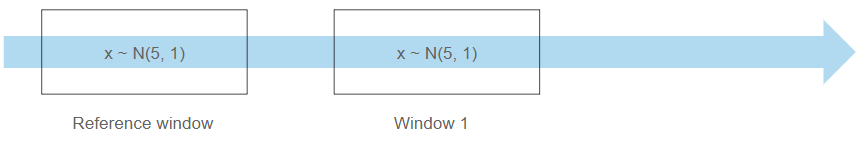
\includegraphics[scale=0.65]{figures/approach2-normality.png}
      \caption[]{Normal state for feature \textit{x} in window 1}
      \label{fig:approach2-initial-state}
    \end{center}
\end{figure}


In Figure \ref{fig:approach2-alert-state}, after further sliding steps of our target sliding window, we obtain \textit{Window 2}. In \textit{Window 2}, the mean and standard deviation aggregation values change from 5 and 1 to 12 and 6, respectively. In this case, we would measure the difference between the target sliding window aggregations and the reference window ones and if above a certain threshold raise an alert. For example, if we used a threshold of $t = 6$, we would raise an alert, as at least one sliding aggregation, in this case the mean, would differ of at least $t$ when compared to the reference value.

\begin{figure}[!htb]
    \begin{center}
      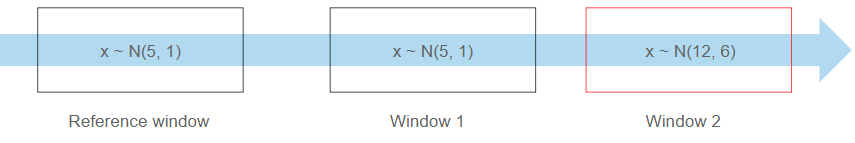
\includegraphics[scale=0.65]{figures/approach2-alert.png}
      \caption[]{Alert state for feature \textit{x} in window 2}
      \label{fig:approach2-alert-state}
    \end{center}
\end{figure}

\subsection*{Challenges}
The first issue with this approach is that generic sliding window aggregation algorithms grow linearly in space regarding window size, such as Recalculate-From-Scratch and Subtract-On-Evict from Section \ref{sec:back-swag-algs}, Two-Stacks from Section \ref{sec:2stacks} and DABA in Section \ref{sec:daba} which does not meet our sub-linear memory growth requirement. 

Exponential Moving Averages (Section \ref{sec:emas}), Probabilistic Data Structures (Section \ref{sec:pds}) and their sliding window implementations (Section \ref{sec:sliding-pds}) can be used to solve this first issue and reduce the linear memory complexity of the system relative to sliding window size. 

Another challenge when using this approach is defining the set of aggregations to compute at feature/variable level that represent the system state well enough for comparison of reference and streaming periods and change detection. To illustrate this problem, consider both time-series show in Figure \ref{fig:approach2-timeseries}. Time-series 1 and 2 have the same maximum, minimum, mean and standard deviation values for the time-based window between \textit{t\textsubscript{1}} and \textit{t\textsubscript{8}}. Hence, if our set of aggregations chosen were the maximum, minimum, mean and standard deviation, we would not differentiate between these two different time-series.

\begin{figure}[!htb]
    \begin{center}
      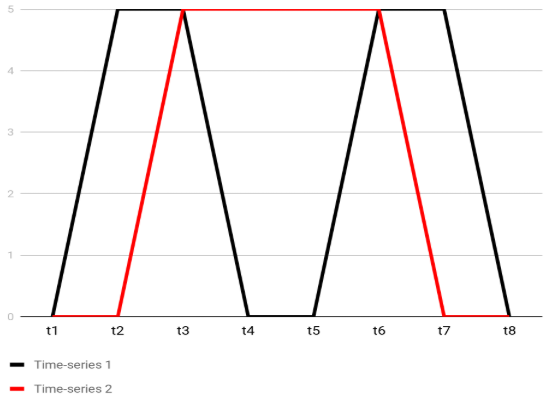
\includegraphics[scale=0.7]{figures/approach2-timeseries.png}
      \caption[]{Two different time-series with same max, min, mean and standard deviation}
      \label{fig:approach2-timeseries}
    \end{center}
\end{figure}

\subsection*{Conclusion}
This approach requires efficient sliding window aggregation state maintenance, which can be done using sliding window probabilistic data structures and/or exponential moving averages. However, the need to choose a set of aggregations to use and the deviation threshold itself ultimately led us to discard this approach.

\section{Method: Feature Distribution Monitoring} \label{sec:ft-monitoring}

In Section \ref{sec:stream-superset}, we defined a data stream as a continuous collection of events. Each event is timestamped and contains multiple fields. In the context of this Thesis, each of the event's fields are named features. Our goal is to detect data pattern shifts for each feature in a streaming fashion. Such shifts will be measured between a static in time or reference period versus the observed reality during the streaming phase. Figure \ref{fig:timelines} shows the separated reference and streaming timelines.

\begin{figure}[!htb]
    \begin{center}
      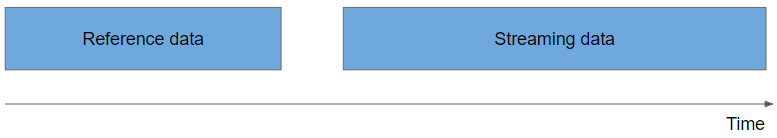
\includegraphics[scale=0.7]{figures/timeperiods.png}
      \caption[]{Reference and streaming timelines}
      \label{fig:timelines}
    \end{center}
\end{figure}


To detect data pattern shifts, we do not need to directly compare the entire window contents of the reference and sliding windows. This approach would require storing all window contents hence making the memory consumption grow linearly with target sliding window and/or reference period size. Instead, we want to use a \textit{(a)} fixed cost in-memory aggregation that can be \textit{(b)} incrementally maintained during the streaming phase. Additionally, we want a streaming aggregation that \textit{(c)} reliably encodes the distribution of each feature. 

One aggregation that encodes distributions properly are histograms. Histograms are a representation of the distribution of numerical data thus being ideal to encode the distribution of feature values, satisfying \textit{(c)}. Histograms require storing a fixed-size list of bins and corresponding counts per bin regardless of the volume of data, satisfying property \textit{(a)}. Adding or removing an element to the histogram aggregation is tantamount to determining the correct bin and incrementing or decrementing the associated count, respectively, thus satisfying property \textit{(b)}. Recall Section \ref{sec:back-swag-algs} where we discussed generic sliding window aggregation algorithms and remember the Subtract-On-Evict (SOE) algorithm (Algorithm \ref{pseudo:soe}). Computing a histogram aggregation over a sliding window of size $W$ using SOE implies storing all $W$ elements in memory to know the element to remove after a new one is inserted. This violates our constant in-memory property \textit{(a)} which is why we chose to use the Exponential Moving Averages (EMAs) analyzed in Section \ref{sec:emas}. EMA-like histograms computed over sliding windows do not require the storage of window contents. An EMA-like histogram is \textit{(a)} constant in memory, \textit{(b)} maintained in real-time and \textit{(c)} encodes the distribution of each feature values. EMA-like histograms are further explained in Section \ref{sec:ema-hist}.

Since the reference window is static, \textit{i.e.}, it is not a sliding window, we can use exact histogram aggregations. Hence, for each feature, we build an exact reference histogram aggregation. On the other hand, in streaming, we use one EMA-like approximate histogram aggregation per feature (Figure \ref{fig:timelines-hists}).


\begin{figure}[!htb]
    \begin{center}
      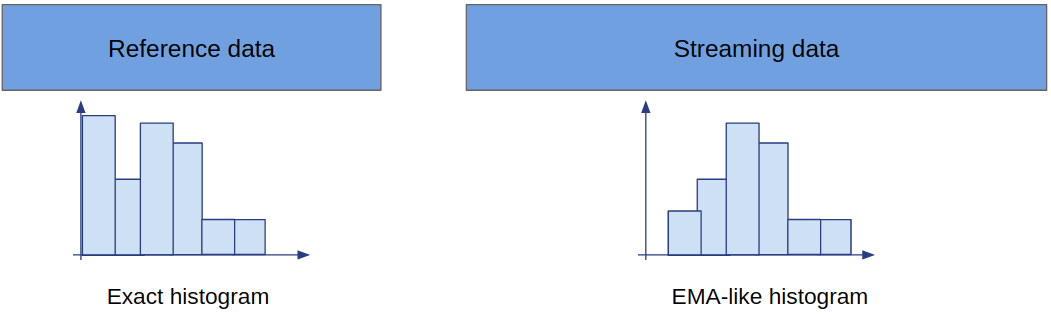
\includegraphics[scale=0.7]{figures/timelines-hists.png}
      \caption[]{Reference and Streaming timelines and corresponding histogram aggregations}
      \label{fig:timelines-hists}
    \end{center}
\end{figure}


To compare each feature's reference and target sliding window histogram aggregation we need a measure of divergence. We chose to use the Jensen–Shannon Divergence (JSD) \cite{JSD} but other statistical tests are possible such as Kolmogorov-Smirnov or Wasserstein \cite{EncyclopaediaMathematics}. The JSD takes as input two histograms and outputs a value between 0 and 1. The closer this value is to 0 the more similar the distributions are. On the other hand, a JSD value of 1 represents two different distributions. We chose to use the JSD metric due to its simplicity and leave as future work other possible tests. 

Given a divergence or distance value for the two aggregations (reference and target) we need a measure of normal statistical fluctuations. Since we consider the reference period as the normal state we can find the normal distribution for the divergence by sampling smaller windows of data from the reference period in a batch analysis. This allows us to define a threshold based on percentiles, which gives an estimate for the probability of a certain value occurring, rather than using a constant hand-picked threshold for the divergence value (details in Section \ref{sec:sampling-batch}). 


To implement the proposed methodology, we devised a two-phase method. The first phase relies on a batch analysis that, for each feature, builds a reference histogram and computes the distribution of divergence values (details presented in Section \ref{sec:batch-phase}). The second phase (detailed in Section \ref{sec:stream-phase}) focuses on efficiently updating the target sliding window histogram for each feature and periodically performing a divergence test between the static reference aggregation and the target sliding one, alerting for changes if need be. The proposed method currently works only for numerical features, that is, only for event fields or variables that are of numeric type, but can be extended to other types.


\subsection{Exponential Moving Average based histogram} \label{sec:ema-hist}
As stated, we compute histogram aggregations for the reference and target sliding windows. The computation of the reference histogram is done once in batch. Since the reference data is fixed and does not change over time, computing this histogram in batch is more efficient and easier to implement in a distributed system like Spark. In addition, a batch computation also allows us to compute an exact reference histogram. However, the target sliding window histogram is an EMA-like histogram to ensure that we are able to encode the feature distribution with constant space complexity and maintain it in real-time.

In Section \ref{sec:emas} we discussed Exponential Moving Averages (EMAs) and how they compute sliding window aggregations without actually storing the window contents. Definition \ref{def:tuple-ema} shows how to compute an EMA using its recursive formula. An EMA state or value depends only on the previous one multiplied by an exponential decay. Recall that a tuple-based decay is given by:
\[ 2^{- \frac{1}{n_{1/2}}} \]
where $n_{1/2}$ is commonly denoted as a tuple-based half-life. 


After processing \textit{x} tuples the oldest tuple is \emph{smoothed} by a factor of $2^{- \frac{x}{n_{1/2}}}$. If we process $x = 4n_{1/2}$ tuples the oldest tuple would have its contribution reduced by
\[ 2^{- \dfrac{4n_{1/2}}{n_{1/2}}} = 2^{-4} \]
which is approximately 0.06. In other words, the \textit{x-th} event would have 6\% contribution towards the EMA state or value meaning older events would have even less weight.

We choose to emulate windows with four times the half-life size (or $4n_{1/2}$), meaning we discard events whose contribution is less than 6\%. We set the half-life to be one-quarter of the size of the window we want to emulate. We want to monitor a period extending up to one month (at an error level of about 6\%) so we set the half-life to be the number of tuples that correspond to one week worth of data. This will give more weight to the most recent week but it will include contributions decaying to 6\% in the fourth oldest week.

\subsection{Batch analysis phase} \label{sec:batch-phase}
\textcolor{red}{TODO: add some pseudocode}

The goal of the batch phase will be to build our reference aggregation for each feature and get to know the distribution of divergence or distance values between the reference and EMA-like aggregations. In other words, we:

\begin{enumerate}
    \item Obtain a reference histogram for each feature using all data in the reference period
    
    \item Compute the distribution of distances between the reference histogram and random windows of data and corresponding histograms
\end{enumerate}

This distribution of values can then later be compared to a given value of divergence for a single sample to find out how probable that value is to occur (if it is very low an alert may be raised).

\subsubsection*{Building the reference histogram for each feature}

First, for each feature, we compute the reference histogram from the reference period dataset. This is an exact histogram aggregation. When building it we ensure the histogram has equal counts (or equal height) for all bins which often results in different sized bins. We make no assumption on the dataset distributions and hence use equal height histograms because they adjust better to wildly varying ones. Equal height means we have more bins covering very dense regions (regions with many data points) and fewer bins in lower density regions. 

\begin{figure}[!htb]
    \begin{center}
      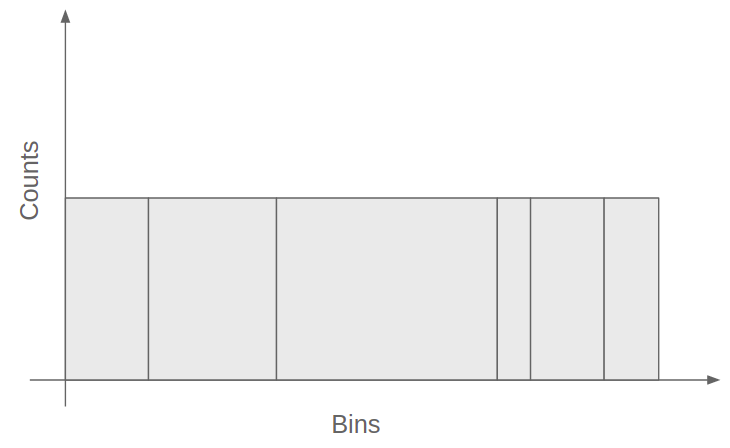
\includegraphics[scale=0.4]{figures/ref-hist.png}
      \caption[]{Reference equal-height histogram}
      \label{fig:ref-hist}
    \end{center}
\end{figure}


\subsubsection*{Finding the distribution of distances for each feature} \label{sec:sampling-batch}

Secondly, we aim to build the histogram that encodes the distribution of expected distance values, to later on threshold the observed distance values during the online phase. To that end, we make $S$ samples of transactions (in Section \ref{sec:nsamples} we discuss the minimum number $S$ of samples to make), each with the same tuple-based size of the target sliding window we will use in streaming. Each sample is a contiguous block of transactions, thus preserving the order of transactions and the time-dependency property of a time-series. 

For each sample, and each feature, we compute the approximated histogram using the bins computed for the reference histogram (Figure \ref{fig:ref-hist-bins}). We also add two extra bins that will cover the region to the left and the right of our histogram, respectively. In other words, we add a bin that covers the region between $-\infty$ and our first bin and another that covers values from the last bin to $+\infty$. This way, observed values outside of the reference period will be placed in these special bins, either left or right.

\begin{figure}[!htb]
    \begin{center}
      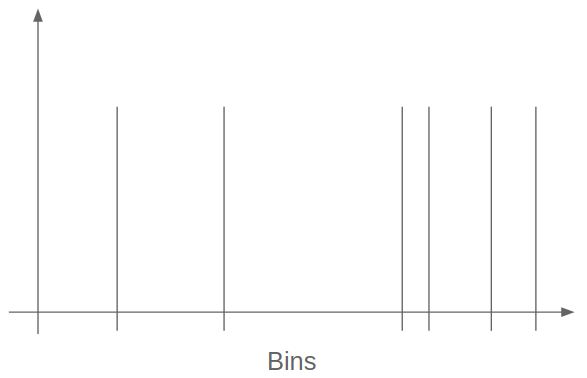
\includegraphics[scale=0.4]{figures/ref-bins.png}
      \caption[]{Reference equal-height histogram}
      \label{fig:ref-hist-bins}
    \end{center}
\end{figure}

Each of the histograms is an EMA-like histogram. An EMA-like histogram is essentially a collection of EMA-counts, as described in Section \ref{sec:ema-hist}. Each sample is processed event by event and a discount factor is applied per event to each bin (EMA expiration factor), thus building an approximated histogram aggregation, using the reference bins, for each feature of that sample. This procedure is illustrated in Figure \ref{fig:EMA-hist-build}.
\begin{figure}[!htb]
    \begin{center}
    \hspace{2cm}
      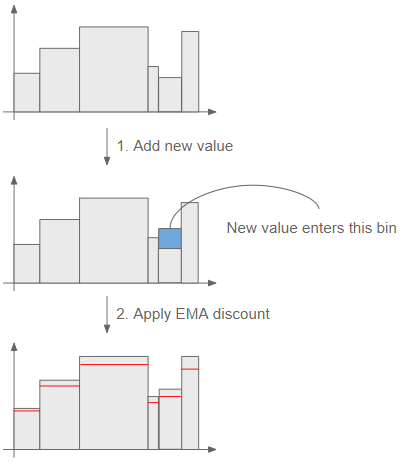
\includegraphics[scale=0.8]{figures/ema-hist.png}
      \caption[]{Reference equal-height histogram}
      \label{fig:EMA-hist-build}
    \end{center}
\end{figure}
We compute multiple sample histograms to encode distributions over smaller time periods that may exist within the large reference period. We use an approximated histogram to mimic the target approximated histogram we will incrementally maintain in the streaming environment.

For each feature, we have now \textit{S} histograms, one for each sample. For each of the \textit{S} histograms, we compute the distance between it and the reference histogram. Figure \ref{fig:compute-sample-distances} illustrates this process as we apply our distance function for each sample histogram and the reference histogram, obtaining \textit{S} distance measurements.

\begin{figure}[!htb]
    \begin{center}
      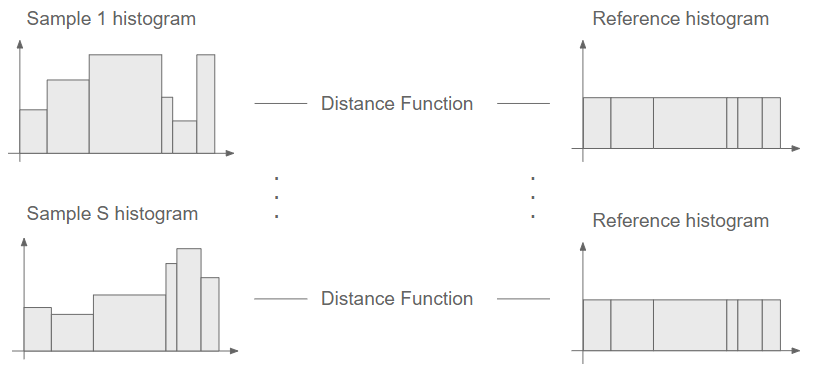
\includegraphics[scale=0.7]{figures/compute-sample-distances.png}
      \caption[Compute as many distance values as samples]{Compute as many distance values as samples, one for each sample-reference histogram pair}
      \label{fig:compute-sample-distances}
    \end{center}
\end{figure}

For each feature, we end up with \textit{S} distance values. These $S$ measurements are distance measurements between random samples of data and the reference period. Hence, we claim we now know the distribution of expected distance values. Given a new distance value measured between another random window and the reference window, we can compute its probability and produce alerts if the probability is below a certain threshold. Note that the histograms for each sample are EMA-like histograms (as detailed in Section \ref{sec:ema-hist}) just like the target sliding window histogram. This ensures a certain degree of fidelity in the test we make in streaming because we measure the divergence between a random sample of data (our streaming histogram or any of the sample's histogram) and the reference one.


It is important to understand why we want to know the distribution of divergence values instead of just thresholding the divergence value itself. For instance, given that JSD values vary between 0 and 1, why not just set to alert if the measured JSD value is 0.7? The reason is that a divergence value may fall on different percentiles for different features. In other words, the same \textit{i-th} percentile will correspond to a different divergence value for different features. Consider the following left and right-skewed distance distributions represented by Figures \ref{fig:skewed-left-distro} and \ref{fig:skewed-right-distro}, respectively. 

\begin{figure}[!htb]
    \begin{center}
      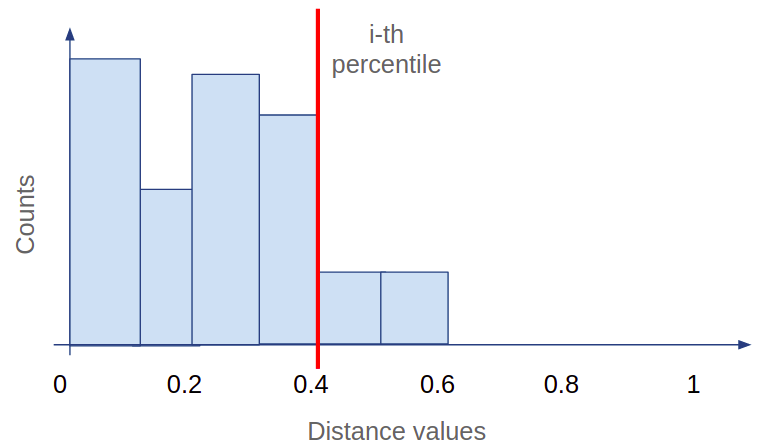
\includegraphics[scale=0.4]{figures/skewed-left-distro.png}
      \caption[]{Left skewed distribution of distance values}
      \label{fig:skewed-left-distro}
    \end{center}
\end{figure}

\begin{figure}[!htb]
    \begin{center}
      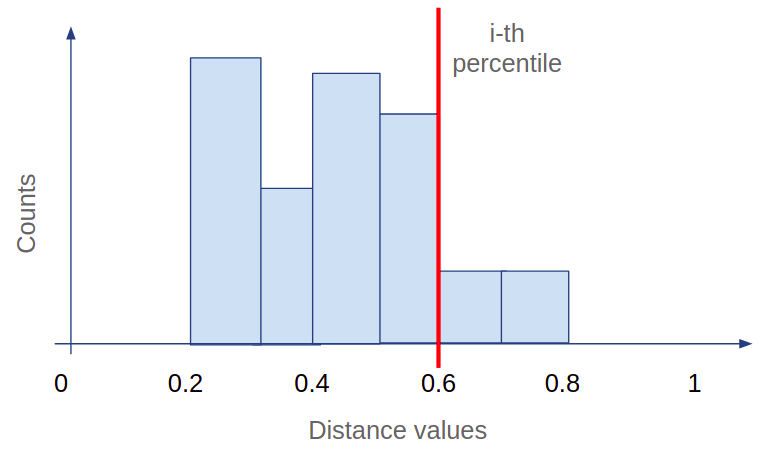
\includegraphics[scale=0.4]{figures/skewed-right-distro.png}
      \caption[]{Right skewed distribution of distance values}
      \label{fig:skewed-right-distro}
    \end{center}
\end{figure}

Let's assume that the histogram from Figure \ref{fig:skewed-left-distro} encodes the distribution of expected distance values for a feature \textit{x1} and Figure \ref{fig:skewed-right-distro} does the same but for a feature \textit{x2}. Setting a user-defined threshold of \textit{$\alpha$=0.6} for both features would yield very different results. For feature \textit{x1} we would be reporting distance values above the 100th-percentile which would not be the case for feature \textit{x2}. Instead, we define our threshold as a percentile of the distribution and not as a hard-coded distance constant. For instance, in this case, we would define the threshold to be the \textit{i}-th percentile, which would correspond to a threshold value of 0.4 for feature \textit{x1} and 0.6 for feature \textit{x2}.

Hard-coding a threshold value to be used for all features is cumbersome, impractical and error-prone. The distance threshold must be computed based on the distribution of distances.


\subsubsection*{Burn-in period at system initialization}
When we boot up our system in the streaming phase we initially have empty histogram aggregations. The period of time where you discard the alerts produced by the system until it processes enough data to produce accurate reports is commonly denoted as the burn-in period. To avoid this burn-in period we propose that the target sliding window approximate histogram aggregation for each feature is initialized using the last sample's histogram for that feature.

\subsubsection*{Batch phase artifacts}
By the end of the batch phase, we should have, for each feature: 
\begin{itemize}
    \item a reference histogram
    \item a list of distance values that represent its distribution
    \item the last sample's histogram, to be used as burn-in period for the target sliding window histogram
\end{itemize}

\subsection{Streaming phase} \label{sec:stream-phase}
\textcolor{red}{TODO: add some pseudocode}

In the streaming or online phase, the system will process event by event in a true sliding window fashion (recall Section \ref{sec:windows}) and perform a change detection test periodically. This phase makes use of all of the batch phase artifacts, namely, for each feature, the reference histogram, the distribution of distance values and the last sample's histogram.

For each feature, we initialize the approximate histogram with the last sample's data, from the batch phase. Then, for each incoming event and each of the event's features, we update our streaming approximate histogram for that feature by adding the new value and then "cutting a slice" from the top of the histogram bars to simulate eviction, as described in Section \ref{sec:ema-hist}. This is all we do, regarding event processing.

In order to obtain alerts, we periodically perform a multi-feature change detection test. The test is done by first computing the distance between the reference histogram for a feature \textit{x} and the target sliding window histogram of the same feature. This distance value is then tested against the known distribution of distance values for feature \textit{x}. In other words, we test to see if the percentile of the computed distance is in the distribution of distance values and alert if above a certain percentile, \textit{e.g.}, the 99th-percentile. When we perform the test, for each feature \textit{x}, we compute the percentile of the distance measured between the reference and target sliding window histogram aggregations. The probability value or \textit{p-value} of a distance value is: 

\[\textit{p-value\textsubscript{distance\textsubscript{x}}} = 1 - percentile(\textit{distance\textsubscript{x}})\]

For example, if we define alerts to have 1\% or less probability to happen, it means the system will raise an alert for distance values above the 99th-percentile or \textit{p-value} = 0.01. Generally speaking, we alert a feature \textit{x} as divergent at a given timestamp if for a given probability threshold $\alpha$:
\[ \textit{percentile(distance\textsubscript{x})} > 1 - \alpha \]
or:
\begin{equation}
    \label{eq:alert-test}
    \textit{p-value\textsubscript{distance\textsubscript{x}}} < \alpha
\end{equation}

\subsubsection*{Multiple Test Correction} \label{sec:multi-test}
Note that we periodically apply this test (Equation \ref{eq:alert-test}) for each feature, effectively repeating the analysis. When considering several hypotheses, the problem of multiplicity arises: the more hypotheses are checked, the higher the probability of obtaining false positives. In other words, when repeating a test multiple times the multiple test or simultaneous statistical inference problem \cite{MultiTestProblem-Pubmed}
\cite{MultiTestProblem-Dickhaus2014}
\cite{MultiTestProblem-Miller1966}  \cite{multiple-test-correction-geoffrey} arises which states that the more inferences are made, the more likely erroneous inferences are to occur. In the literature, many multiple test correction methods are proposed, but we opted to use the Holm-Bonferroni multiple test correction due to its simplicity and ease of computation and leave as future work the testing of other correction methods. In statistics, Family-Wise Error Rate (FWER) \cite{MultivariateMT} \cite{MultitestTamhane2018AdvancesIP} is the probability of making one or more false positives when performing multiple hypotheses tests, \textit{i.e.}, consider one hypothesis true when it is not. The Holm-Bonferroni method \cite{HolmBonferroni} is one of many approaches for controlling the Family-Wise Error Rate \textit{(FWER)} by adjusting the rejection criteria for each hypothesis.


\subsubsection*{Holm-Bonferroni Correction} \label{sec:holmbonferroni}
The Holm-Bonferroni correction takes Equation \ref{eq:alert-test} and corrects the right-side threshold $\alpha$ for each feature. This correction is done by dividing the threshold $\alpha$ by a correction factor, as described next.

First, we compute the \textit{p-value} of each feature. We then order our features by \textit{p-value}, in ascending order. Next, starting from the first feature, the one with the smallest \textit{p-value}, and proceeding until the end of the list of features, we check if:
\[  \textit{p-value\textsubscript{distance\textsubscript{x}}} < \alpha / (\textit{m} - \textit{k}) \]
with $\alpha$ as the probability to reject the null hypothesis, \textit{m} as the number of hypotheses to test, in our case the number of features and corresponding \textit{p-values} and \textit{k} as the 0-based index of the current feature. We stop at the first feature that fails this test, and every feature processed up until this one is considered to be a divergent feature and alerts are raised.

\subsection{Final remarks}

\subsubsection*{Minimum number of samples} \label{sec:nsamples}
In Section \ref{sec:sampling-batch} we stated we made \textit{S} samples in the batch phase. But what is the optimal number of samples to make? How can we mathematically derive a formula for the number of samples to make and avoid \textit{ad hoc} user-defined constants?

When checking for alerts we are performing one test for each feature, hence we perform \textit{n\textsubscript{features}} tests. We apply a multiple test correction on the tests performed and want to set the FWER to $\alpha$. In other words, we want to alert deviations for the full set of tests globally that have probability $\alpha$ < 1\%, for example.

We use the Holm-Bonferroni correction and, for each feature, we need to reliably estimate the upper tail of the distribution which corresponds to the \textit{$\alpha$ / n\textsubscript{features}} region. Each sample we do translates into a distance value and the collection of these data points builds the distribution of distance values. We want to be sure that the number of samples \textit{S} that we do generates enough distance points to have a high probability of having one or more points in the upper tail region. To that end, we define the probability of not having at least one point in the upper tail of the distance distribution as $\gamma$. 

In \cite{SAMM}, the authors prove that the minimum number of samples $S$ needed to satisfy these probability requirements is:
\begin{equation}
    \label{eq:optimal-n-samples}
    \textit{S} = \ceil[\bigg]{\frac{\log\gamma}{log(1 - \frac{\alpha}{n_{features}})}}
\end{equation}

\chapter{Method Validation} \label{chap:validation} \minitoc

In this section, we provide summary statistics for our method's performance and draw visualizations for the obtained results to validate our alarms and reason about them.

\section{Experiments with Synthetic Data}
In order to test our proposed system, we generated multiple synthetic datasets before moving on to real data. In this section we present summary statistics for the synthetic datasets created and our generated alarms.

\subsection{Single Feature Analysis}
As an initial step, we started by validating our system using single-feature datasets before moving to multi-feature scenarios to facilitate system validation, considering the complexities of multi-feature datasets and the problem of multiple test correction. In this section we validate our results for single-feature synthetic datasets.

\subsubsection{Varying Sample Sizes}
We began with single-feature scenarios and by experimenting with different tuple-based half-lives $n_{1/2}$. The half-life $n_{1/2}$ parameter in turn controls the size of the samples we make in the batch phase and the target sliding window size of the streaming phase. 

In Section \ref{sec:ema-hist}, we mentioned that we choose to discard events whose contribution is less than 6\%. We set a half-life $n_{1/2}$ value and then multiply it by a constant factor of 4 to get the size of the samples to make (a larger sample would contain events whose contribution was equal to or less than 6\%). 

All the synthetic datasets used throughout this section are a time-series where at each time-step we sample uniformly from a fixed distribution, \textit{i.e.} there are no time correlations in the used datasets. The reference dataset R1 used in this first experiment contained a single feature that followed a normal distribution with mean $\mu=10$ and standard deviation $\sigma=2$ for the 5 million rows of the dataset. Figure \ref{fig:timeseries-r1} shows the time-series of the single feature in dataset R1. The dataset processed in the streaming phase (\textit{i.e.} the target dataset) was generated with a size of 5 million events and a single feature. For the first half, \textit{i.e.}, for the first 2.5 million events, the feature followed a normal distribution with mean $\mu=10$ and standard deviation $\sigma=2$, like the reference dataset. For the other half, we changed the generating distribution to be a continuous uniform one with lower bound $a=100$ and upper bound $b=200$. Figure \ref{fig:timeseries-t1} shows the time-series of the single feature in the target dataset T1 where we see the abrupt change in feature values.
\begin{center}
\begin{minipage}{.5\textwidth}
  \centering
  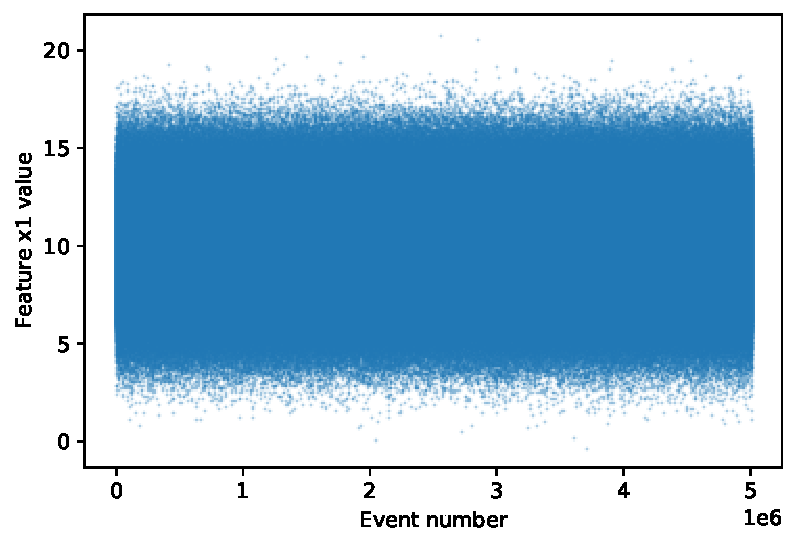
\includegraphics[width=1\linewidth]{figures/01-reference.pdf}
  \captionof{figure}{Time-series for dataset R1}
  \label{fig:timeseries-r1}
\end{minipage}%
\begin{minipage}{.5\textwidth}
  \centering
  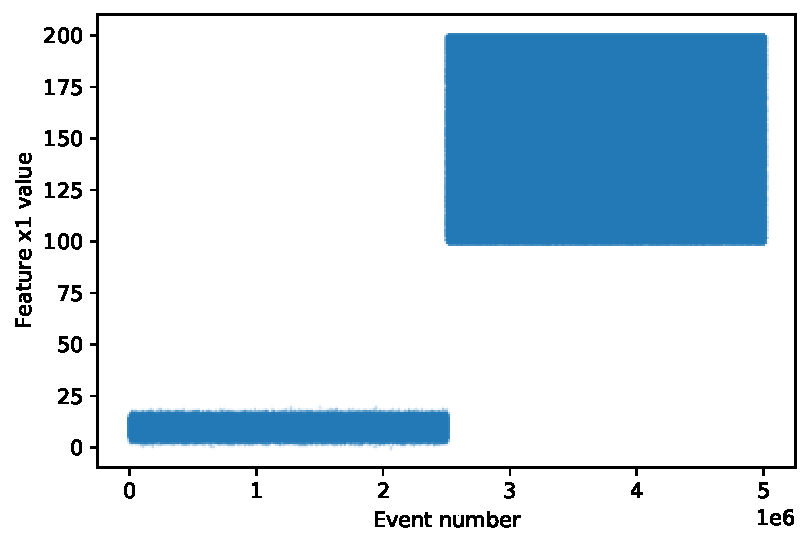
\includegraphics[width=1\linewidth]{figures/01-target.pdf}
  \captionof{figure}{Time-series for dataset T1}
  \label{fig:timeseries-t1}
\end{minipage}
\end{center}

We conducted three different experiments varying the tuple-based half-life $n_{1/2}$, using the reference dataset R1 and the target dataset T1. The experiment identifiers, the corresponding half-lives and the execution times are shown in Table \ref{tbl:tests-half-life}. Notice that $Sample Size$ corresponds to the size of each sample made in the batch phase and so it is four times the half-life. We used 100 bins (plus the two special infinity bins) for the reference histogram and made 1000 samples.
\begin{table}[!htb]
    \begin{center}
        \begin{tabular}{|c|c|c|c|c|}
        \hline
        \multicolumn{1}{|l|}{\textbf{Experiment}} & \multicolumn{1}{l|}{\textbf{Half-life}} & \multicolumn{1}{l|}{\textbf{Sample Size}} & \multicolumn{1}{l|}{\textbf{Executors}} & \multicolumn{1}{l|}{\textbf{Batch execution time (seconds)}} \\ \hline
        01                                        & 625                                     & 2500                                      & 300                                     & 152                                                          \\ \hline
        02                                        & 62,500                                  & 250,000                                   & 300                                     & 2,822                                                        \\ \hline
        03                                        & 250,000                                 & 1,000,000                                 & 300                                     & 10,082                                                       \\ \hline
        \end{tabular}
    \end{center}
    \caption{Experiments with varying half-life}
    \label{tbl:tests-half-life}
\end{table}
Table \ref{tbl:tests-half-life} shows the execution time for the batch phase in seconds. All experiments used 300 Spark executor instances. From the Table we conclude that the larger the half-life, the larger the sample size. Larger samples imply longer processing times when computing the EMA-like histogram for each sample. With no surprise, we see that the larger the sample the longer it takes to finish the batch phase.

From a functional point of view, were we able to detect the abrupt change introduced in the target dataset T1? Recall that from the 2.5 millionth event forward we change the distribution from a gaussian to an uniform one (Figure \ref{fig:timeseries-t1}). Figure \ref{fig:JSD-signal-01} shows the distance (JSD) values computed during streaming at each event of the 5 million events from dataset T1, using the outputs from the batch phase of experiment 01. We clearly see a change in JSD values, and we move from values close to 0 to values close to 1 (or even 1). Figure \ref{fig:JSD-signal-zoom-01} shows the same signal but for the first half of the streaming period (essentially a zoom-in). We see our JSD values before the change were very low (magnitudes of $10^{-2}$).
\begin{figure}[!htb]
\centering
\begin{subfigure}{.5\textwidth}
  \centering
  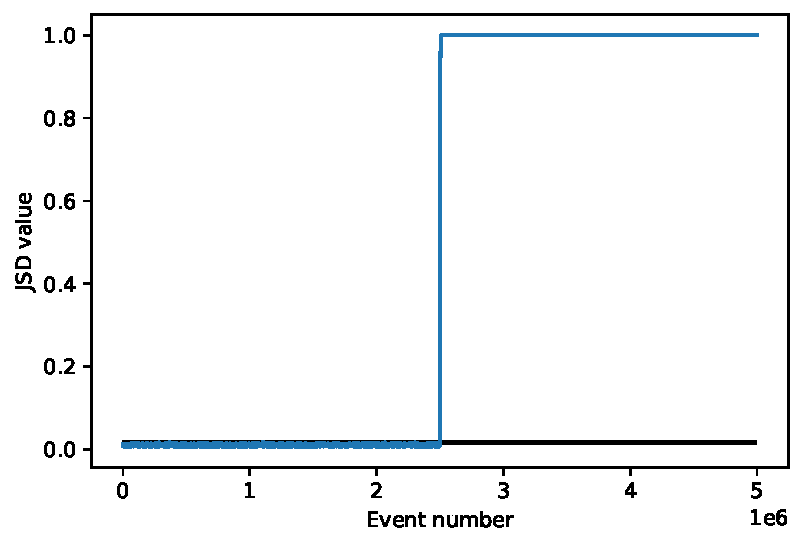
\includegraphics[width=1\linewidth]{figures/stream-analysis-viz-625.pdf}
  \caption{For the whole time-series}
  \label{fig:JSD-signal-01}
\end{subfigure}%
\begin{subfigure}{.5\textwidth}
  \centering
  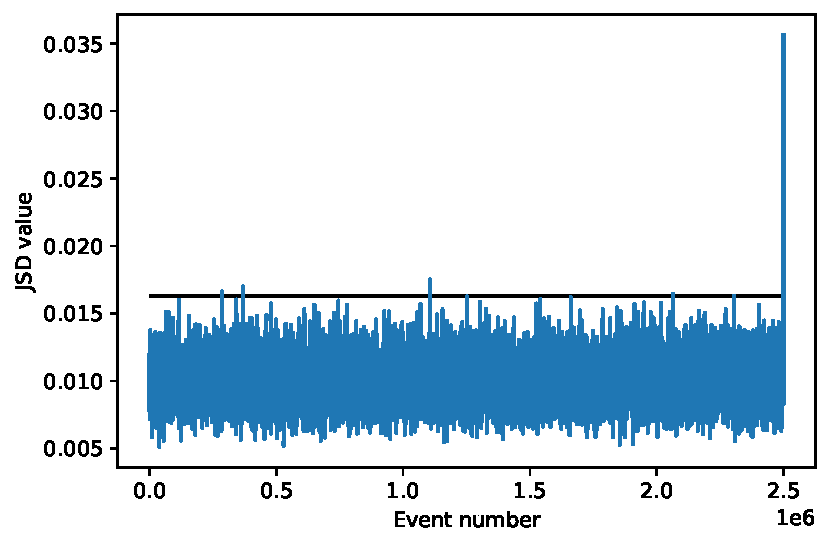
\includegraphics[width=1\linewidth]{figures/stream-analysis-viz-zoom-625.pdf}
  \caption{Zoom in on the first 2.5 million events}
  \label{fig:JSD-signal-zoom-01}
\end{subfigure}
\caption{Experiment 01: JSD signal and threshold}
\end{figure}

However, the change in JSD value is very abrupt as well. Almost instantly we go from close to 0 values to 1. We also had some false-positives, \textit{i.e.}, some JSD values above the threshold. This indicates to us that the window used is too small and sensitive to small changes, or that we can choose a more strict threshold.

In experiment 02, we use larger sampling windows. Remember our target sliding window in streaming is of the same size as the sampling windows. In the second experiment, we increase the size of the sampling and target windows by 100 times.

Figure \ref{fig:JSD-signal-02} shows the JSD signal during streaming for dataset T1, using the outputs from the batch phase of experiment 02. Again, we see a change in signal from the middle of the streaming period forward. Figure \ref{fig:JSD-signal-zoom-02} shows the same signal for the first half of the streaming period.
\begin{figure}[!htb]
\centering
\begin{subfigure}{.5\textwidth}
  \centering
  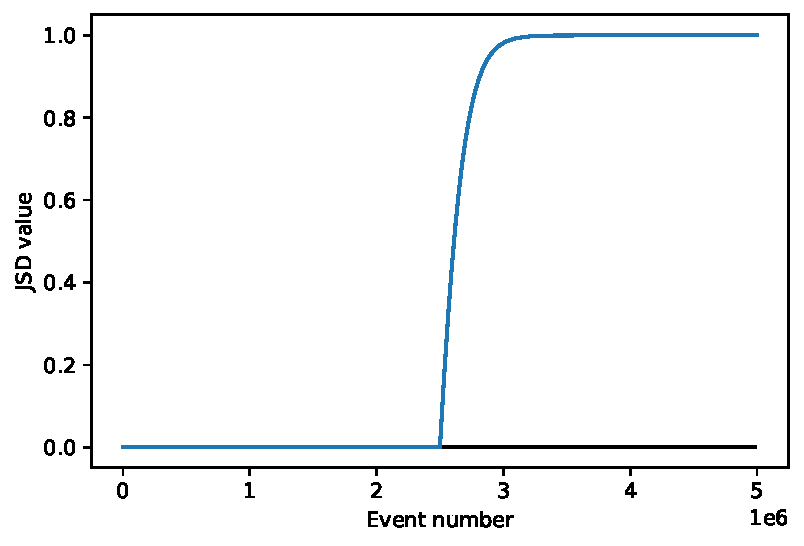
\includegraphics[width=1\linewidth]{figures/stream-analysis-viz-62500.pdf}
  \caption{For the whole time-series}
  \label{fig:JSD-signal-02}
\end{subfigure}%
\begin{subfigure}{.5\textwidth}
  \centering
  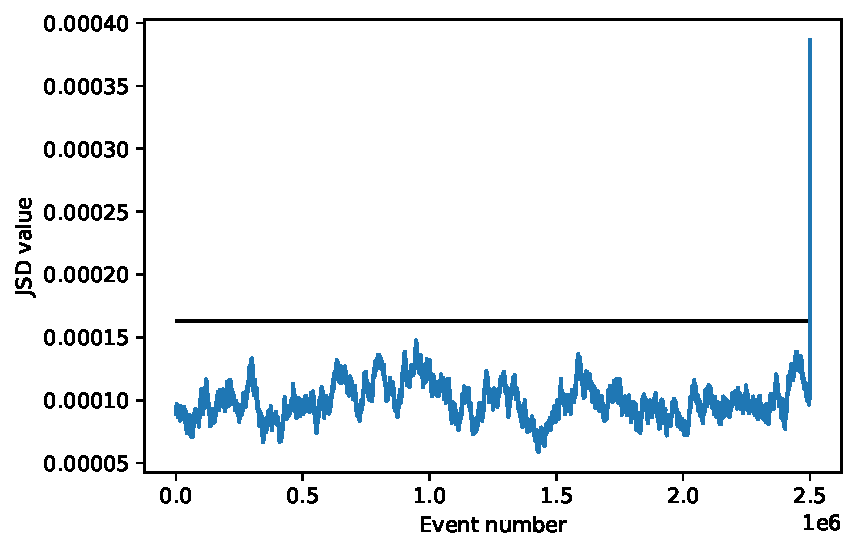
\includegraphics[width=1\linewidth]{figures/stream-analysis-viz-zoom-62500.pdf}
  \caption{Zoom in on the first 2.5 million events}
  \label{fig:JSD-signal-zoom-02}
\end{subfigure}
\caption{Experiment 02: JSD signal and threshold}
\end{figure}
Notice that this time the growth of our signal is slower. Notice also that we do not have false positives in the first half of the signal. This is because we use a larger window, which means each event has a smaller contribution to the aggregation state. Hence, outliers will have less impact on the aggregation and corresponding signal value.

In experiment 03, we increase the sampling and target windows size once again, this time four times larger than in experiment 02. We would expect an even smoother growth of our signal and, again, no false positives. And indeed, judging by the corresponding signal computation and zoom-in, Figures \ref{fig:JSD-signal-03} and \ref{fig:JSD-signal-zoom-03}, respectively, the signal looks smoother and we see no false positives.
\begin{figure}[!htb]
\centering
\begin{subfigure}{.5\textwidth}
  \centering
  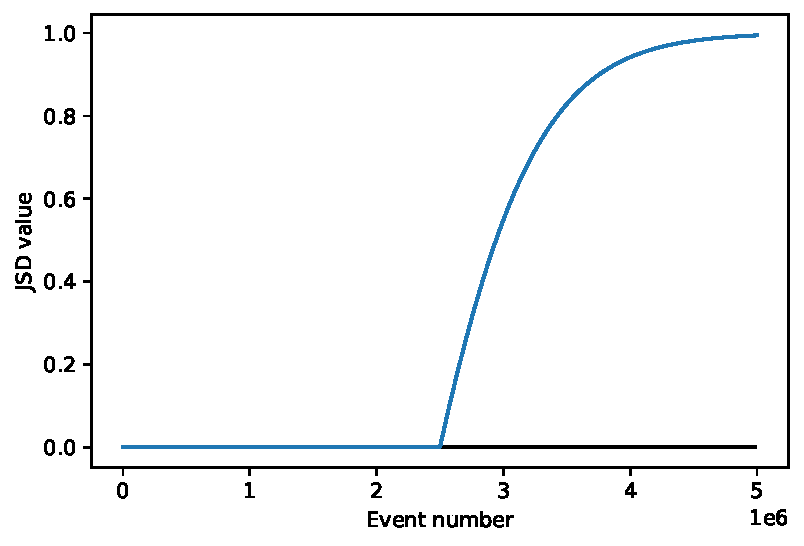
\includegraphics[width=1\linewidth]{figures/stream-analysis-viz-250000.pdf}
  \caption{For the whole time-series}
  \label{fig:JSD-signal-03}
\end{subfigure}%
\begin{subfigure}{.5\textwidth}
  \centering
  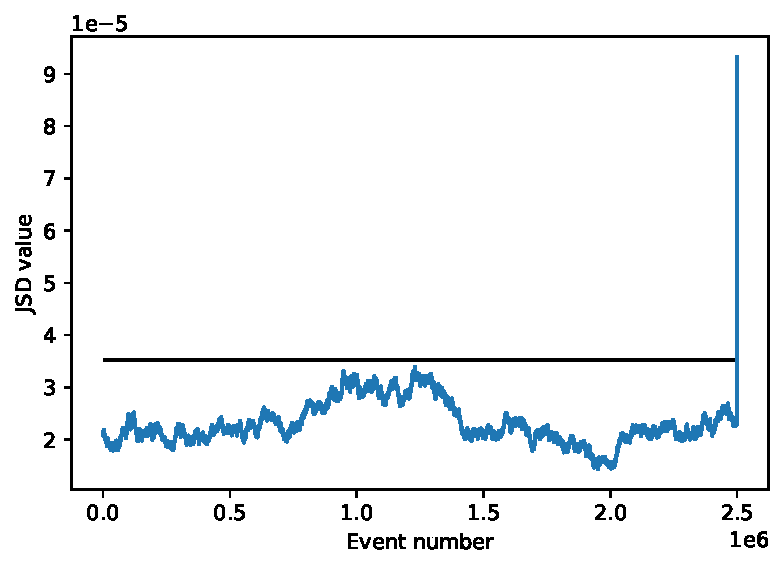
\includegraphics[width=1\linewidth]{figures/stream-analysis-viz-zoom-250000.pdf}
  \caption{Zoom in on the first 2.5 million events}
  \label{fig:JSD-signal-zoom-03}
\end{subfigure}
\caption{Experiment 03: JSD signal and threshold}
\end{figure}


\subsubsection{Multiple Distribution Changes}
In this experiment, we wanted to see how our signal behaved when there were multiple change points, where each gaussian distribution was a scaled down version of the previous one. Figure \ref{fig:timeseries-r2} shows the time-series for the reference dataset R2 used in this experiment. It contained 5 million events with a single feature following a gaussian distribution with mean $\mu=100$ and standard deviation $\sigma=50$. The time-series for target dataset T2 is shown in Figure \ref{fig:timeseries-t2}. Notice that we change distributions at 2, 3 and 4 millionth events. Notice also that each subsequent distribution produces values whose domain is a subset of the previous distribution.
\begin{center}
\begin{minipage}{.5\textwidth}
  \centering
  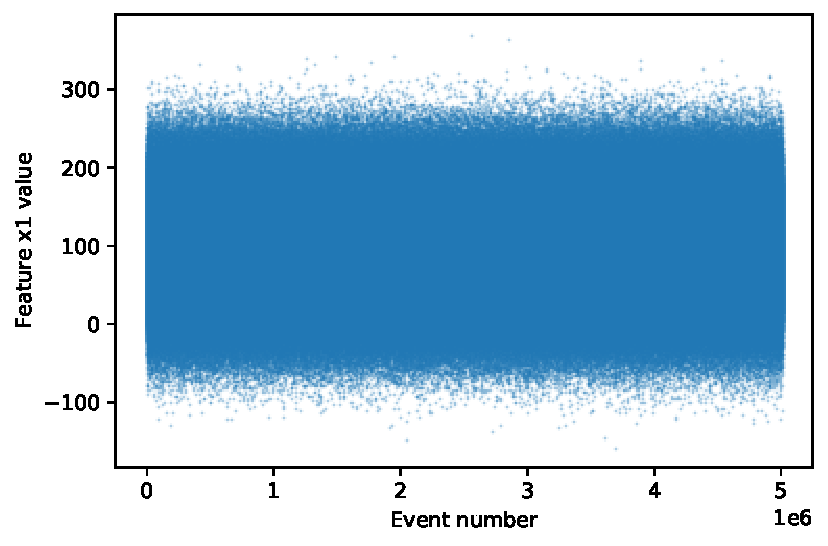
\includegraphics[width=1\linewidth]{figures/timeseries-r2.pdf}
  \captionof{figure}{Time-series for dataset R2}
  \label{fig:timeseries-r2}
\end{minipage}%
\begin{minipage}{.5\textwidth}
  \centering
  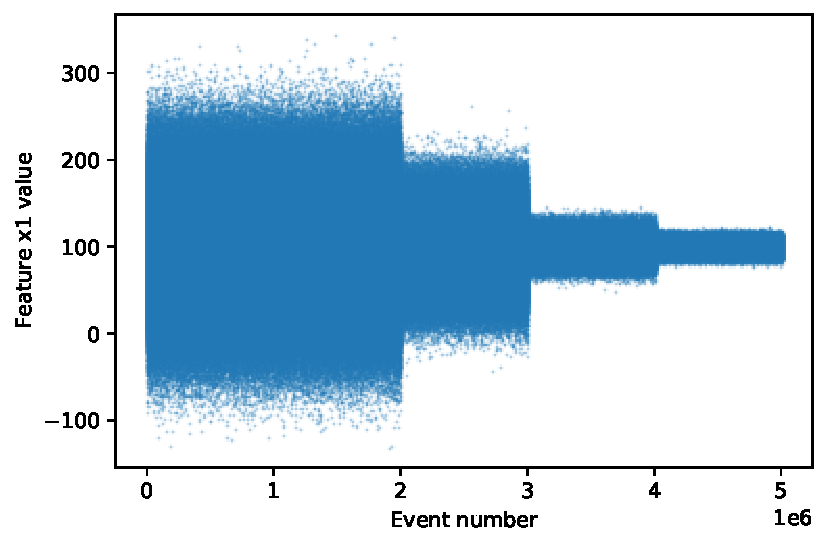
\includegraphics[width=1\linewidth]{figures/timeseries-t2.pdf}
  \captionof{figure}{Time-series for dataset T2}
  \label{fig:timeseries-t2}
\end{minipage}
\end{center}

The target dataset T2 begins with the same distribution as the reference dataset R2, a gaussian distribution with mean $\mu=100$ and standard deviation $\sigma=50$. At the 2 millionth event mark, we use another Gaussian distribution, this time with mean $\mu=100$ and standard deviation $\sigma=30$. At the 3 millionth event, we change the standard deviation to be $\sigma=10$. From the 4 millionth event to the end, we use a standard deviation of $\sigma=5$. 

In this experiment, we used a half-life $n_{1/2}=62500$ and corresponding sample size of 250,000 events, like in the previous Section' experiment 02. Figure \ref{fig:JSD-signal-test02} shows the computed JSD signal for the target dataset and Figure \ref{fig:JSD-signal-zoom-test02} zooms in on the first 2 millionth events, before any distribution is changed. We observe that once again we have no false positives in the first 2 million events, which is ideal. 
\begin{figure}[!htb]
\centering
\begin{subfigure}{.5\textwidth}
  \centering
  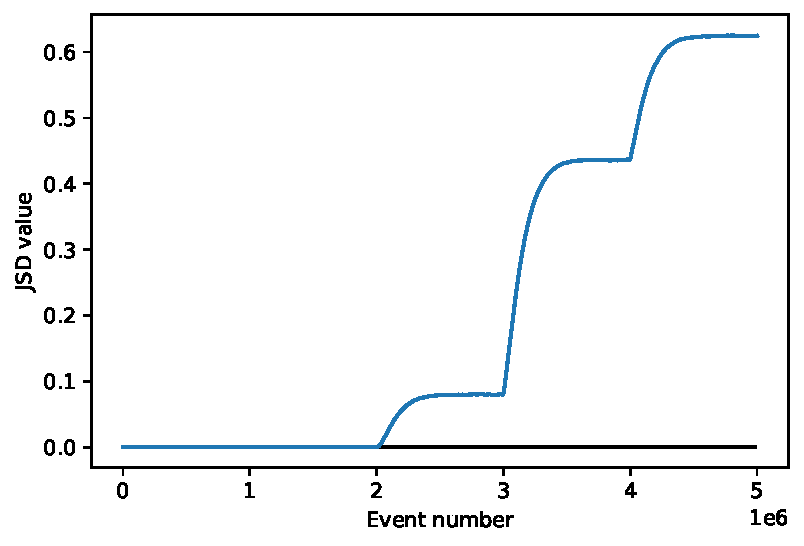
\includegraphics[width=1\linewidth]{figures/stream-analysis-viz-test02.pdf}
  \caption{For the whole time-series}
  \label{fig:JSD-signal-test02}
\end{subfigure}%
\begin{subfigure}{.5\textwidth}
  \centering
  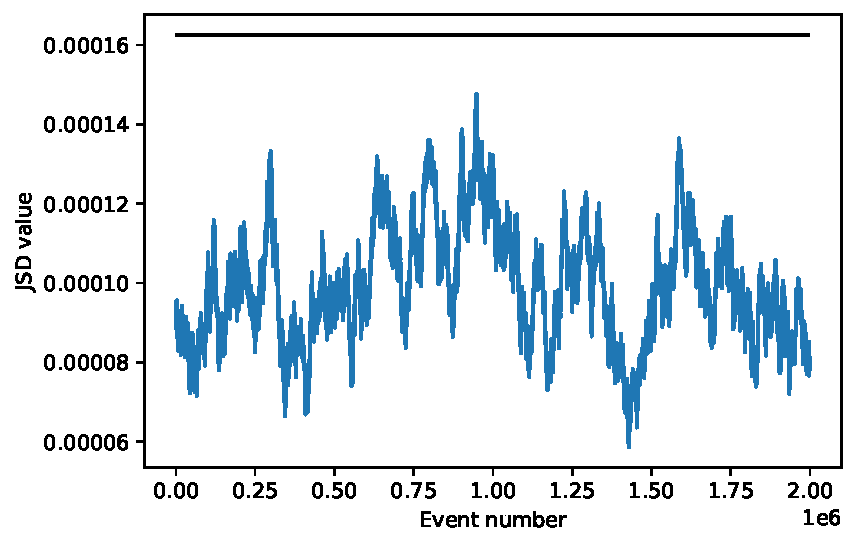
\includegraphics[width=1\linewidth]{figures/stream-analysis-viz-zoom-test02.pdf}
  \caption{Zoom in on the first 2 million events}
  \label{fig:JSD-signal-zoom-test02}
\end{subfigure}
\caption{JSD signal and threshold}
\end{figure}
Furthermore, we observe that the computed JSD signal varies accordingly with the changes in distribution. Despite us changing the distributions to subsets of the previous ones to try and deceive our method, our signal accurately represents these changes. In Figure \ref{fig:JSD-signal-test02}, we see several growth points that correspond to the points where the generating gaussian distribution parameters changed. Hence, we are able to detect changes in distribution parameter changes and quantify how big the change is (the closer to 1 our signal is).

\subsubsection{Multiple Distribution Changes, each a Superset of the Previous One}
In this experiment, we wanted to do the reverse of the previous one. In this one, there are multiple change points but each new distribution spans a domain that is a superset of the previous one. Figure \ref{fig:timeseries-r3} shows the reference period used, with 5 million events and one feature following a gaussian distribution of mean $\mu=100$ and standard deviation $\sigma=10$. Figure \ref{fig:timeseries-t3} shows the target period used, also with 5 million events and one feature. Like in the previous experiment, we change distributions at the 2, 3 and 4 millionth event mark. On the other hand, unlike the previous experiment, we now make subsequent distributions cover the previous ones. We change the reference gaussian used with mean $\mu=100$ and standard deviation $\sigma=10$ at the 2, 3 and 4 millionth mark, to use standard deviations $\sigma=30$, $\sigma=40$ and $\sigma=50$, respectively.
\begin{center}
\begin{minipage}{.5\textwidth}
  \centering
  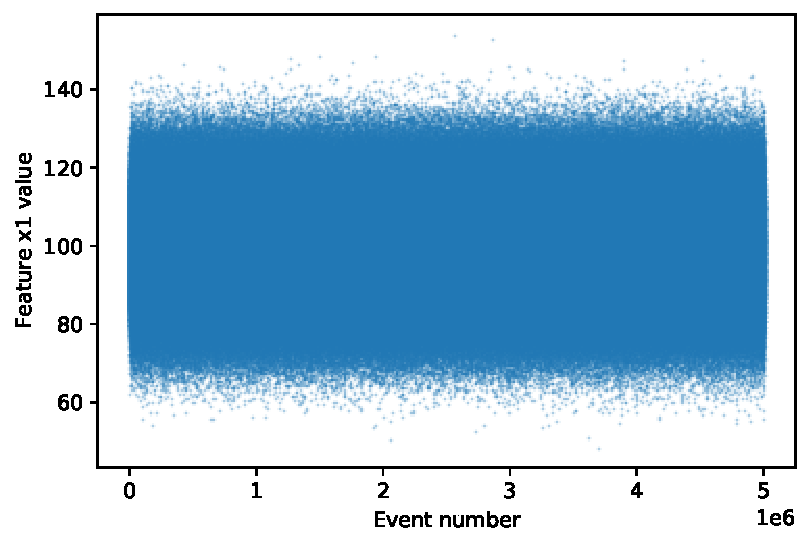
\includegraphics[width=1\linewidth]{figures/timeseries-r3.pdf}
  \captionof{figure}{Time-series for dataset R3}
  \label{fig:timeseries-r3}
\end{minipage}%
\begin{minipage}{.5\textwidth}
  \centering
  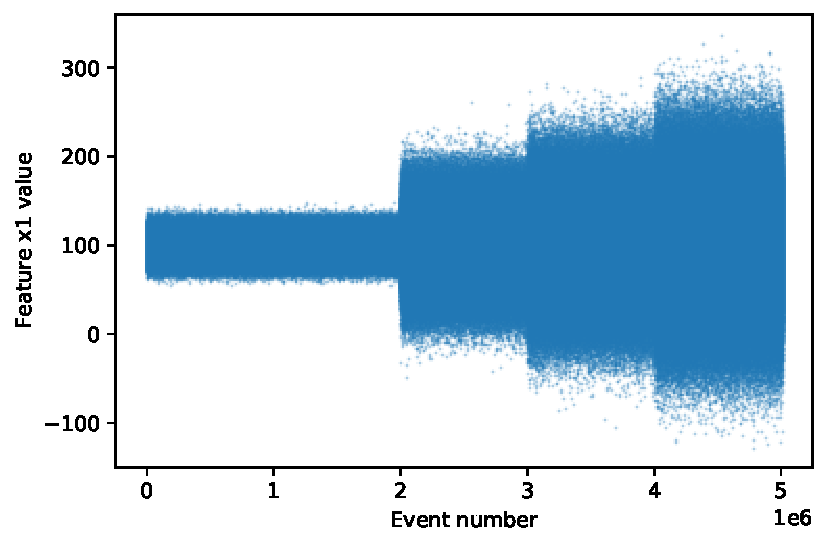
\includegraphics[width=1\linewidth]{figures/timeseries-t3.pdf}
  \captionof{figure}{Time-series for dataset T3}
  \label{fig:timeseries-t3}
\end{minipage}
\end{center}

Figure \ref{fig:JSD-signal-test03} shows the JSD signal for the target dataset in this experiment. Once again, we were able to detect the changes introduced at the 2, 3 and 4 millionth events. We are also able to identify bigger distribution changes, relative to the reference, by observing bigger JSD values. Figure \ref{fig:JSD-signal-zoom-test03} shows a zoomed in portion of the original signal, where we can verify that there are no false positives.
\begin{figure}[!htb]
\centering
\begin{subfigure}{.5\textwidth}
  \centering
  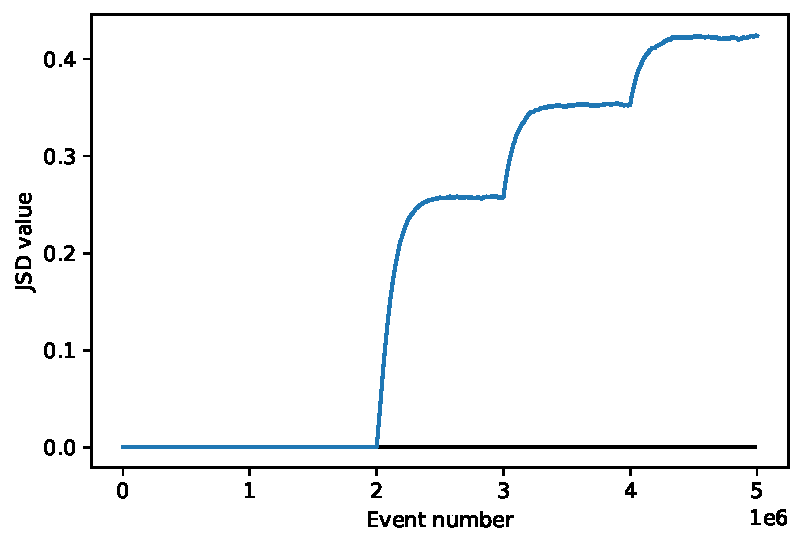
\includegraphics[width=1\linewidth]{figures/stream-analysis-viz-test03.pdf}
  \caption{For the whole time-series}
  \label{fig:JSD-signal-test03}
\end{subfigure}%
\begin{subfigure}{.5\textwidth}
  \centering
  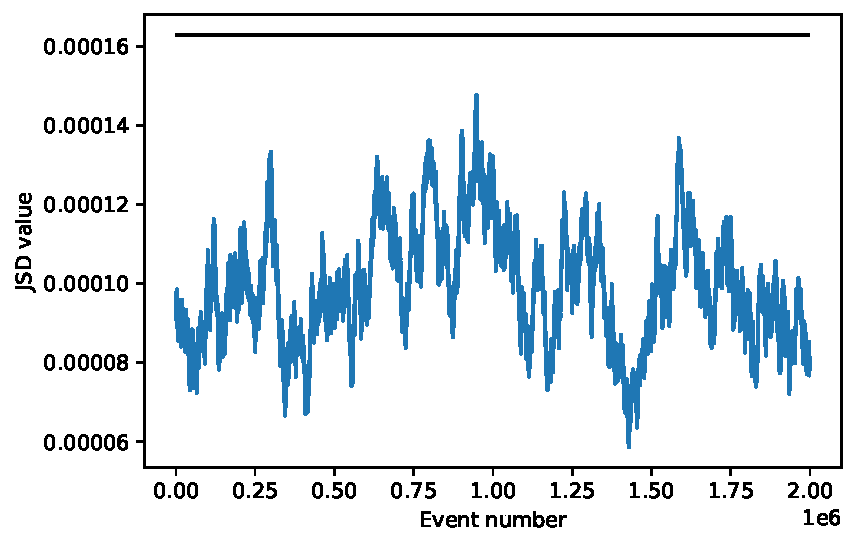
\includegraphics[width=1\linewidth]{figures/stream-analysis-viz-zoom-test03.pdf}
  \caption{Zoom in on the first 2 million events}
  \label{fig:JSD-signal-zoom-test03}
\end{subfigure}
\caption{JSD signal and threshold}
\end{figure}

\subsubsection{Return to Normality After Change}
Our goal with this experiment was to check if our signal returned to its normal values (below the alert threshold) if we changed our distribution to the original reference one, as intended.

In this experiment, we used reference dataset R4 (Figure \ref{fig:timeseries-r4}) and target dataset T4 (Figure \ref{fig:timeseries-t4}). 
\begin{center}
\begin{minipage}{.5\textwidth}
  \centering
  \includegraphics[width=1\linewidth]{figures/timeseries-r4.pdf}
  \captionof{figure}{Time-series for dataset R4}
  \label{fig:timeseries-r4}
\end{minipage}%
\begin{minipage}{.5\textwidth}
  \centering
  \includegraphics[width=1\linewidth]{figures/timeseries-t4.pdf}
  \captionof{figure}{Time-series for dataset T4}
  \label{fig:timeseries-t4}
\end{minipage}
\end{center}

The reference dataset R4 had a single feature that followed a Gaussian distribution of $\mu=100$ and $\sigma=5$ for all 5 million events. Up until the 2 millionth event, the target dataset T4 followed a Gaussian distribution of $\mu=100$ and $\sigma=5$, similarly to the reference dataset R4. At the 2 millionth event, we change the Gaussian parameters to $\mu=100$ and $\sigma=30$. At the 3 millionth mark, we once again change the Gaussian parameters to $\mu=100$ and $\sigma=50$. Finally, on the 4 millionth event, we return to our reference distribution, a gaussian with $\mu=100$ and $\sigma=5$.


Figure \ref{fig:JSD-signal-test04} shows the computed JSD signal for the target period. As expected, our JSD signal increases at the 2 millionth and 3 millionth event mark, because the distribution parameters change. At the 4 millionth event, we use the original reference distribution and notice that the JSD signal returns to values below the threshold, considering it a normal state, as we intended. Figure \ref{fig:JSD-signal-zoom-test04} is a zoom in on the first 2 millionth events before any change occurs, and we see no false positives.

\begin{figure}[!htb]
\centering
\begin{subfigure}{.5\textwidth}
  \centering
  \includegraphics[width=1\linewidth]{figures/stream-analysis-viz-test04.pdf}
  \captionof{figure}{JSD signal and threshold}
  \label{fig:JSD-signal-test04}
\end{subfigure}%
\begin{subfigure}{.5\textwidth}
  \centering
  \includegraphics[width=1\linewidth]{figures/stream-analysis-viz-zoom-test04.pdf}
  \caption{Zoom in on the first 2 million events}
  \label{fig:JSD-signal-zoom-test04}
\end{subfigure}
\caption{JSD signal and threshold}
\end{figure}


\subsubsection{An Attempt to Deceive our Method}
In this experiment, we attempt to deceive our method by using a different distribution from the reference period but ensuring its domain is roughly the same as the reference one.

We used the reference dataset R5 (Figure \ref{fig:timeseries-r5}) which had 5 million events, with a single-feature that followed a gaussian with  $\mu=100$ and $\sigma=10$. Our target dataset T5 is represented in Figure \ref{fig:timeseries-t5}. For the first 2 million events, the generating distribution used was similar to the one used in the reference dataset, a gaussian with $\mu=100$ and $\sigma=10$. However, at the 2 millionth event, we change the gaussian standard deviation to $\sigma=30$. Then, at the 4 millionth event, we change the distribution type. We use an uniform distribution with lower bound $a=80$ and upper bound $b=120$. Note in Figure \ref{fig:timeseries-t5} that this last portion resembles the first one, the reference.
\begin{center}
\begin{minipage}{.5\textwidth}
  \centering
  \includegraphics[width=1\linewidth]{figures/timeseries-r5.pdf}
  \captionof{figure}{Time-series for dataset R5}
  \label{fig:timeseries-r5}
\end{minipage}%
\begin{minipage}{.5\textwidth}
  \centering
  \includegraphics[width=1\linewidth]{figures/timeseries-t5.pdf}
  \captionof{figure}{Time-series for dataset T5}
  \label{fig:timeseries-t5}
\end{minipage}
\end{center}

Let's take a look at the signal computed for the target period. Figure \ref{fig:JSD-signal-test05} shows us the JSD signal for dataset T5 (Figure \ref{fig:timeseries-t5}). As expected, we see a rapid growth of JSD value after the 2 millionth event, when we change the Gaussian parameters. We then change the distribution type, from a gaussian to a uniform one. Despite the latter having a domain contained within the former, we see that our signal is accurate and does not drop below the alert threshold. This is still a different distribution that we want to alert. Figure \ref{fig:JSD-signal-zoom-test05} is a zoom in of the first 2 millionth events and once again we have no false positives.
\begin{figure}[!htb]
\centering
\begin{subfigure}{.5\textwidth}
  \centering
  \includegraphics[width=1\linewidth]{figures/stream-analysis-viz-test05.pdf}
  \captionof{figure}{JSD signal and threshold}
  \label{fig:JSD-signal-test05}
\end{subfigure}%
\begin{subfigure}{.5\textwidth}
  \centering
  \includegraphics[width=1\linewidth]{figures/stream-analysis-viz-zoom-test05.pdf}
  \caption{Zoom in on the first 2 million events}
  \label{fig:JSD-signal-zoom-test05}
\end{subfigure}
\caption{JSD signal and threshold}
\end{figure}

\subsection{Multi Feature Analysis}
Before moving to real data, we performed one last experiment, using synthetic data but this time performing a multi-feature analysis. Table \ref{tbl:multi-feat-ref-dataset-distros} shows the underlying generating distributions and parameters for each of the four features ($x_1$, $x_2$, $x_3$ and $x_4$) in the reference multi-feature dataset R6. Figures \ref{fig:timeseries-r6-x1}, \ref{fig:timeseries-r6-x2}, \ref{fig:timeseries-r6-x3} and \ref{fig:timeseries-r6-x4} show the reference time-series for features $x_1$, $x_2$, $x_3$ and $x_4$ on the reference dataset R6, respectively.

\begin{table}[!htb]
    \begin{center}
        \begin{tabular}{|c|c|c|ll}
        \cline{1-3}
        \textbf{Feature} & \textbf{Reference Distribution} & \textbf{Parameters} &  &  \\ \cline{1-3}
        x1               & Gaussian/Normal                 & $\mu=100$, $\sigma=5$  &  &  \\ \cline{1-3}
        x2               & Gaussian/Normal                 & $\mu=100$, $\sigma=5$  &  &  \\ \cline{1-3}
        x3               & Uniform                         & $a=200$, $b=250$       &  &  \\ \cline{1-3}
        x4               & Uniform                         & $a=50$, $b=125$        &  &  \\ \cline{1-3}
        \end{tabular}
    \end{center}
    \caption{Multi feature reference dataset and feature distributions}
    \label{tbl:multi-feat-ref-dataset-distros}
\end{table}


\begin{figure}[!htb] 
  \begin{minipage}[b]{0.5\linewidth}
    \centering
    \includegraphics[width=1\linewidth]{figures/timeseries-r6-x1.pdf} 
    \caption{Feature x1 reference time-series} 
    \label{fig:timeseries-r6-x1} 
    \vspace{4ex}
  \end{minipage}%%
  \begin{minipage}[b]{0.5\linewidth}
    \centering
    \includegraphics[width=1\linewidth]{figures/timeseries-r6-x2.pdf} 
    \caption{Feature x2 reference time-series} 
    \label{fig:timeseries-r6-x2} 
    \vspace{4ex}
  \end{minipage} 
  \begin{minipage}[b]{0.5\linewidth}
    \centering
    \includegraphics[width=1\linewidth]{figures/timeseries-r6-x3.pdf} 
    \caption{Feature x3 reference time-series} 
    \label{fig:timeseries-r6-x3} 
    \vspace{4ex}
  \end{minipage}%% 
  \begin{minipage}[b]{0.5\linewidth}
    \centering
    \includegraphics[width=1\linewidth]{figures/timeseries-r6-x4.pdf} 
    \caption{Feature x4 reference time-series} 
    \label{fig:timeseries-r6-x4} 
    \vspace{4ex}
  \end{minipage} 
\end{figure}

We used a target dataset T6 with 5 million events and the same four features ($x_1$, $x_2$, $x_3$ and $x_4$). Feature x1 followed the reference distribution for the 5 million events of the target dataset. We did not change this feature underlying distribution to serve as a control, \textit{i.e.}, we expect no alerts for this one. Figure \ref{fig:timeseries-t6-x1} shows the time-series for the target dataset T6 and feature $x_1$.

Feature x2's underlying distribution changed four times and returned to normal, so we expect to see alarms with increasing divergence values but eventually no more alarms. Figure \ref{fig:timeseries-t6-x2} shows the time-series for the target dataset T6 and feature $x_2$. Feature $x_2$ followed a gaussian with $\mu=100$ and $\sigma=5$ like in the reference period up to the 1 millionth event mark, then a gaussian with $\mu=100$ and $\sigma=10$ up to the 2.5 millionth event, then a gaussian $\mu=100$ and $\sigma=15$ until the 3 millionth event, then a gaussian $\mu=100$ and $\sigma=20$ until the 4 millionth event and finally returned to the original gaussian with $\mu=100$ and $\sigma=5$ until the last event. Table \ref{tbl:multi-feat-x2-changes} sums up the distributions used and its parameters for each interval of the reference dataset for feature x2.
\begin{table}[!htb]
    \begin{center}
    \begin{tabular}{|c|c|c|c|l}
    \cline{1-4}
    \textbf{From Event} & \textbf{To Event} & \textbf{Distribution} & \multicolumn{1}{l|}{\textbf{Parameters}} &  \\ \cline{1-4}
    0                   & 1,000,000         & Gaussian              & $\mu=100, \sigma=5$                      &  \\ \cline{1-4}
    1,000,000           & 2,500,000         & Gaussian              & $\mu=100, \sigma=10$                     &  \\ \cline{1-4}
    2,500,000           & 3,000,000         & Gaussian              & $\mu=100, \sigma=15$                     &  \\ \cline{1-4}
    3,000,000           & 4,000,000         & Gaussian              & $\mu=100, \sigma=20$                      &  \\ \cline{1-4}
    4,000,000           & 5,000,000         & Gaussian              & $\mu=100, \sigma=5$                      &  \\ \cline{1-4}
    \end{tabular}
    \end{center}
    \caption{Feature x2 generating distributions}
    \label{tbl:multi-feat-x2-changes}
\end{table}

Feature x3's underlying distribution changed three times and never returned to normal, so we expect to see alarms with increasing divergence values up until the end of the stream analysis. Figure \ref{fig:timeseries-t6-x3} shows the time-series for the target dataset T6 and feature x3. Feature x3 followed a uniform distribution with $a=200$ and $b=250$ like in the reference period up to the 1.5 millionth event mark, then a uniform distribution with $a=200$ and $b=220$ up to the 2 millionth event, then a uniform distribution with $a=180$ and $b=200$ until the 3.5 millionth event and finally a gaussian with $\mu=50$ and $\sigma=20$ until the last event. Table \ref{tbl:multi-feat-x3-changes} sums up the distributions used and its parameters for each interval of the reference dataset for feature x3.
\begin{table}[!htb]
    \begin{center}
    \begin{tabular}{|c|c|c|c|l}
    \cline{1-4}
    \textbf{From Event} & \textbf{To Event} & \textbf{Distribution} & \multicolumn{1}{l|}{\textbf{Parameters}} &  \\ \cline{1-4}
    0                   & 1,500,000         & Uniform               & $a=200, b=250$                           &  \\ \cline{1-4}
    1,500,000           & 2,000,000         & Uniform               & $a=200, b=220$                           &  \\ \cline{1-4}
    2,000,000            & 3,500,000         & Uniform               & $a=180, b=200$                           &  \\ \cline{1-4}
    3,500,000           & 5,000,000         & Gaussian              & $\mu=50, \sigma=20$                      &  \\ \cline{1-4}
    \end{tabular}
    \end{center}
    \caption{Feature x3 generating distributions}
    \label{tbl:multi-feat-x3-changes}
\end{table}

Feature x4's underlying distribution changed two times and returned to normal, so we expect to see no alarms towards the end of the stream analysis. Figure \ref{fig:timeseries-t6-x4} shows the time-series for the target dataset T6 and feature x4. Feature x4 followed a uniform distribution like the reference one, with $a=50$ and $b=125$ up until the 1.5 millionth event. After that, it followed a uniform distribution with $a=125$ and $b=200$ until the 3 millionth event where it resumed its original uniform distribution (with $a=50$ and $b=125$) until the end. Table \ref{tbl:multi-feat-x4-changes} sums up the distributions used and its parameters for each interval of the reference dataset for feature x4.
\begin{table}[!htb]
    \begin{center}
    \begin{tabular}{|c|c|c|c|l}
    \cline{1-4}
    \textbf{From Event} & \textbf{To Event} & \textbf{Distribution} & \multicolumn{1}{l|}{\textbf{Parameters}} &  \\ \cline{1-4}
    0                   & 1,500,000         & Uniform               & $a=50, b=125$                            &  \\ \cline{1-4}
    1,500,000           & 3,000,000         & Uniform               & $a=125, b=200$                           &  \\ \cline{1-4}
    3,000,000           & 5,000,000         & Uniform               & $a=50, b=125$                            &  \\ \cline{1-4}
    \end{tabular}
    \end{center}
    \caption{Feature x4 generating distributions}
    \label{tbl:multi-feat-x4-changes}
\end{table}


\begin{figure}[!htb] 
  \begin{minipage}[b]{0.5\linewidth}
    \centering
    \includegraphics[width=1\linewidth]{figures/timeseries-t6-x1.pdf} 
    \caption{Feature x1 target time-series} 
    \label{fig:timeseries-t6-x1} 
    \vspace{4ex}
  \end{minipage}%%
  \begin{minipage}[b]{0.5\linewidth}
    \centering
    \includegraphics[width=1\linewidth]{figures/timeseries-t6-x2.pdf} 
    \caption{Feature x2 target time-series} 
    \label{fig:timeseries-t6-x2} 
    \vspace{4ex}
  \end{minipage} 
  \begin{minipage}[b]{0.5\linewidth}
    \centering
    \includegraphics[width=1\linewidth]{figures/timeseries-t6-x3.pdf} 
    \caption{Feature x3 target time-series} 
    \label{fig:timeseries-t6-x3} 
    \vspace{4ex}
  \end{minipage}%% 
  \begin{minipage}[b]{0.5\linewidth}
    \centering
    \includegraphics[width=1\linewidth]{figures/timeseries-t6-x4.pdf} 
    \caption{Feature x4 target time-series} 
    \label{fig:timeseries-t6-x4} 
    \vspace{4ex}
  \end{minipage} 
\end{figure}

In this experiment, we used a tuple-based half-life $n_{1/2}=62500$, \textit{i.e.} sampling and target windows of 250,000 tuples. We used 100 bins for the reference histogram plus the two special infinity bins. In this multi-feature scenario, we used the Holm-Bonferroni correction discussed in Section \ref{sec:holmbonferroni} and set the Family-Wise Error Rate (FWER) to 1\% (FWER = 0.01). Furthermore, instead of doing 1000 samples as we did previously in an ad-hoc way, we use Equation \ref{eq:optimal-n-samples} to determine the minimum number of samples to make while ensuring $\gamma=1\%$ (recall Section \ref{sec:nsamples}). For our four feature analysis scenario, using as inputs  $\gamma=0.01$ and $FWER=0.01$ in Equation \ref{eq:optimal-n-samples} tells us we need to make 1840 samples minimum. Using 300 Spark executors, each given 3G of memory, we finished the batch phase in 418 seconds.

In Section \ref{sec:stream-phase}, we mention that, in our stream analysis, we perform our multiple hypothesis divergence tests on a fixed user-defined frequency. Finding an optimal frequency value for the test falls out of scope for this Thesis, but ideally, we set it to be large enough so that we do fewer computations and achieve higher throughput but still get alerts in useful time. In this experiment, we performed the divergence test with the Holm-Bonferroni correction \ref{sec:holmbonferroni} for every new event (frequency of 1 event). We did this to collect a list of ordered corrected p-values for each feature. A corrected p-value (derived from Equation \ref{eq:corrected-pvalue}) is given by:
\begin{equation}
    p-value_{corrected} = p-value_{distance_{x}} * (m - k)
    \label{for:corrected-pvalue}
\end{equation}
With this list, for each feature, we can plot the corrected p-values on each event and compare it with the FWER threshold $\alpha$. Note that despite performing the test at the maximum frequency (in real-time) we still achieved a throughput of 17,921 transactions per second (TPS), even if only for four features.

In the following plots, unlike the JSD signal plots presented before, a feature is in a divergent state if its p-value is below the threshold, according to Equation \ref{eq:corrected-pvalue}. Working with corrected p-values (Formula \ref{for:corrected-pvalue}), a feature is considered divergent if its corrected p-value is below the threshold.

In Figure \ref{fig:x1-corrected-pvalues} we see the plot of corrected p-values for feature x1 and the probability threshold black horizontal line at the bottom. Recall that feature x1' values were generated by a Gaussian distribution for both the reference period (Figure \ref{fig:timeseries-r6-x1}) and the target period (Figure \ref{fig:timeseries-t6-x1}), with the same parameters. We observe that the corrected p-values never pass below the threshold, as we expected. Hence, this feature is never alerted as divergent.
\begin{figure}[!htb]
    \begin{center}
      \includegraphics[scale=0.8]{figures/x1-corrected-pvalues.png}
      \caption{Feature x1 corrected p-values and threshold}
      \label{fig:x1-corrected-pvalues}
    \end{center}
\end{figure}

Figure \ref{fig:x2-corrected-pvalues} shows a plot of feature x2's corrected p-values and the FWER threshold. Feature x2 underlying distribution was changed four times (Table \ref{tbl:multi-feat-x2-changes}): at the 1, 2.5, 3 and 4 millionth events. The first change is consistent with the sudden drop in corrected p-value for this feature, as we cross below the threshold and enter a divergent state. Around a thousand events after the change we saw p-values of 0.2\% (or 0.002). The values keep dropping as time passes and as we introduce bigger changes in distribution.
\begin{figure}[!htb]
    \begin{center}
      \includegraphics[scale=0.8]{figures/x2-corrected-pvalues.png}
      \caption{Feature x2 corrected p-values and threshold}
      \label{fig:x2-corrected-pvalues}
    \end{center}
\end{figure}
We resume the reference or original distribution at the 4 millionth event. However, as we can see from a close-up on the original plot (Figure \ref{fig:x2-corrected-pvalues-zoom}), it takes around 600,000 events for the target sliding histogram aggregation to once again resemble the reference one, resulting in a high enough p-value and thus stop alerting x2 as divergent.
\begin{figure}[!htb]
    \begin{center}
      \includegraphics[scale=0.8]{figures/x2-corrected-pvalues-zoom2.png}
      \caption{Feature x2 zoomed in corrected p-values and threshold}
      \label{fig:x2-corrected-pvalues-zoom}
    \end{center}
\end{figure}


Feature x3 was the only feature that never returned to its original distribution and is the only one that should be reported until the end as divergent. This is in fact the case as illustrated in Figure \ref{fig:x3-corrected-pvalues}. The first change to x3's generating distribution was introduced at the 1.5 millionth event and we clearly see the corrected p-value rapidly approaching values close to zero. For the rest of the dataset, this x3's p-value remains below the threshold, as we never swap to its original distribution.
\begin{figure}[!htb]
    \begin{center}
      \includegraphics[scale=0.8]{figures/x3-corrected-pvalues.png}
      \caption{Feature x3 corrected p-values and threshold}
      \label{fig:x3-corrected-pvalues}
    \end{center}
\end{figure}


Finally, feature x4's corrected p-value plot is given by Figure \ref{fig:x4-corrected-pvalues}. Similarly to feature x2, we resume the original distribution at a certain point, in this case at the 3-millionth event. However, as we can see from a close-up on the original plot (Figure \ref{fig:x4-corrected-pvalues-zoom}), it takes around 810,000 events for the target sliding window aggregation to be considered similar enough to the reference one and stop alerting x4 as divergent.
\begin{figure}[!htb]
    \begin{center}
      \includegraphics[scale=0.8]{figures/x4-corrected-pvalues.png}
      \caption{Feature x4 corrected p-values and threshold}
      \label{fig:x4-corrected-pvalues}
    \end{center}
\end{figure}
\begin{figure}[!htb]
    \begin{center}
      \includegraphics[scale=0.8]{figures/x4-corrected-pvalues-zoom2.png}
      \caption{Feature x4 zoomed in corrected p-values and threshold}
      \label{fig:x4-corrected-pvalues-zoom}
    \end{center}
\end{figure}


With this experiment, we further validate that the p-value is a measure of how divergent a feature is: the closer to zero, the lower the probability of the statistical test result and hence the more divergent a feature is considered to be. At the 1.5 millionth event, we swap both x3 and x4's distribution. For the first 2,535,000 events, x4 has a lower p-value than x3 and hence is considered more divergent. However, after that, we change x3's distribution so aggressively that x3 starts being reported as most divergent, with a lower p-value than x4.

\clearpage
\section{Experiments with Real Data}

Due to time constraints, we experimented with data from only one merchant. The merchant's entity as well as feature names will remain anonymous due to confidentiality reasons.

Feedzai provides a fraud detection solution for this merchant and had stored two contiguous in time datasets of credit card transactions that, combined, covered a period of roughly 1 year and 9 months. In this experiment, we used the older one as the reference dataset and the more recent one as the target period. Both datasets were already feature-engineered \cite{Domingos-ML-Feat-Eng} and had a total of 183 numerical plus numerically encoded categorical features (\textit{e.g.} one-hot encoded or ordinal encoded \cite{categoricalencoding}). Table \ref{tbl:merchant1-datasets-summary} shows summary statistics for both datasets.
\begin{table}[!htb]
    \begin{center}
        \begin{tabular}{|c|c|c|c|}
        \hline
        \textbf{Dataset} & \textbf{From}              & \textbf{To}           & \multicolumn{1}{l|}{\textbf{Transactions}} \\ \hline
        Reference        & Tuesday, September 5, 2017 & Friday, June 29, 2018 & 1,604,509                                  \\ \hline
        Target           & Friday, June 29, 2018      & Sunday, June 30, 2019 & 4,032,505                                  \\ \hline
        \end{tabular}
        \caption{Summary statistics for reference and target merchant datasets}
        \label{tbl:merchant1-datasets-summary}
    \end{center}
\end{table}

In the batch phase, we used 100 Spark executors, each with 12G of memory. We determined that one week's worth of data for this merchant was on average equivalent to 37,803 events. We set the half-life to be $n_{1/2}=37,803$ and discard events whose EMA weight is 6\% or less, which is equivalent to using sampling windows of data of four times the half-life (as detailed in Section \ref{sec:ema-hist}). Hence, our samples' windows had 151,212 events. Using Equation \ref{eq:optimal-n-samples}, we determined that for 183 features, a FWER of 1\% and $\gamma$ (as defined in Section \ref{sec:nsamples}) of 10\% we needed to make a minimum of 42,137 samples. Our batch analysis took 5 hours and 34 minutes.

After the batch phase, we had the necessary inputs for the streaming phase (detailed in Section \ref{sec:batch-artifacts-summary}), namely, for each feature, the reference histograms, the list of observed divergence values and the last sample's histogram. We then used the target dataset, simulating a stream of ordered events. Our monitoring system processed the dataset event by event in sequential, time-ordered fashion, emulating a stream computation and reported divergent features with associated p-values. We performed our multiple hypotheses with the Holm-Bonferroni correction (Section \ref{sec:holmbonferroni}) for every 1000 events. It took us 382,363 milliseconds (roughly 6 minutes) to process the 4,032,505 transactions, amounting to a throughput of 10,546 transactions per second (TPS).

This merchant and in particular these datasets were known to suffer a lot from concept drift. Our system produced a large list of alerts, from nearly the beginning of the target period until the end. Due to a large number of features (183), we only show some plots. Furthermore, we refer to features with anonymized identifiers, like feature $x_j$. In the following plots, we show the corrected p-values (Formula \ref{for:corrected-pvalue}) for some features at each event of the time-series and the FWER threshold set at 1\%. A feature is considered divergent at a given timestamp if below that threshold line.

Figure \ref{fig:merchant-x1-reference} is a plot of the reference time-series of feature $x_1$ and Figure \ref{fig:merchant-x1-target} the corresponding target time-series.
\begin{figure}[!htb]
    \begin{center}
      \includegraphics[scale=0.5]{figures/merchant-x1-reference.pdf}
      \caption{Merchant feature x1 reference time-series}
      \label{fig:merchant-x1-reference}
    \end{center}
\end{figure}
\begin{figure}[!htb]
    \begin{center}
      \includegraphics[scale=0.5]{figures/merchant-x1-target.pdf}
      \caption{Merchant feature x1 target time-series}
      \label{fig:merchant-x1-target}
    \end{center}
\end{figure}
In Figure \ref{fig:merchant-x1-correctedpvalues} we plot the corrected p-values for the each event of the target period. The reference and target periods look very similar and in fact we have very few alarms for this feature, \textit{i.e.}, the number of times the line crosses to the bottom half of the plot, imposed by the threshold line. 
\begin{figure}[!htb]
    \begin{center}
      \includegraphics[scale=0.5]{figures/merchant-x1-correctedpvalues.pdf}
      \caption{Merchant feature x1 corrected p-values}
      \label{fig:merchant-x1-correctedpvalues}
    \end{center}
\end{figure}
Furthermore, the alarms appear to be roughly in the middle portion of the time-series, where in fact the target period appears to have less points. We can see roughly three alarms. The first one in early January 2019 for a few days, the second one lasting about a week at the end of January 2019 and the last one in the second half of February 2019 again for a few days.

Now let us look at features $x_2$ and $x_3$. Figures \ref{fig:merchant-x2-reference} and \ref{fig:merchant-x2-target} show feature $x_2$' time-series plots for the reference and target periods, respectively.
\begin{figure}[!htb]
    \begin{center}
      \includegraphics[scale=0.5]{figures/merchant-x2-reference.pdf}
      \caption{Merchant feature x2 reference time-series}
      \label{fig:merchant-x2-reference}
    \end{center}
\end{figure}
\begin{figure}[!htb]
    \begin{center}
      \includegraphics[scale=0.5]{figures/merchant-x2-target.pdf}
      \caption{Merchant feature x2 target time-series}
      \label{fig:merchant-x2-target}
    \end{center}
\end{figure}
Figures \ref{fig:merchant-x3-reference} and \ref{fig:merchant-x3-target} show feature $x_3$' time-series plots for the reference and target periods, respectively.
\begin{figure}[!htb]
    \begin{center}
      \includegraphics[scale=0.5]{figures/merchant-x3-reference.pdf}
      \caption{Merchant feature x3 reference time-series}
      \label{fig:merchant-x3-reference}
    \end{center}
\end{figure}
\begin{figure}[!htb]
    \begin{center}
      \includegraphics[scale=0.5]{figures/merchant-x3-target.pdf}
      \caption{Merchant feature x3 target time-series}
      \label{fig:merchant-x3-target}
    \end{center}
\end{figure}
\clearpage
Relative to $x_1$, features $x_2$ and $x_3$ also have very similar reference and target periods. Just like feature x1, we expect to have some alarms but still not too many. Once again, to visualize the alarms, we plot the corrected p-values for each event of the target time-series for each feature. Figure \ref{fig:merchant-x2-correctedpvalues} is a plot of feature x2' corrected p-values and the FWER threshold of 1\%. Likewise, Figure \ref{fig:merchant-x3-correctedpvalues} shows the same plot but for feature x3.
\begin{figure}[!htb]
    \begin{center}
      \includegraphics[scale=0.5]{figures/merchant-x2-correctedpvalues.pdf}
      \caption{Merchant feature x2 corrected p-values}
      \label{fig:merchant-x2-correctedpvalues}
    \end{center}
\end{figure}
\begin{figure}[!htb]
    \begin{center}
      \includegraphics[scale=0.5]{figures/merchant-x3-correctedpvalues.pdf}
      \caption{Merchant feature x3 corrected p-values}
      \label{fig:merchant-x3-correctedpvalues}
    \end{center}
\end{figure}
The corrected p-values plot shows us once again that both $x_2$ and $x_3$ features had some alarms but eventually rose above the threshold and resumed their reference distribution. This is expected from features whose reference and target time-series plots look so similar.

Next, we analyze a feature with very different reference and target time-series. Feature x4' reference time-series is presented in Figure \ref{fig:merchant-x4-reference} and its target period in Figure \ref{fig:merchant-x4-target}.
\begin{figure}[!htb]
    \begin{center}
      \includegraphics[scale=0.5]{figures/merchant-x4-reference.pdf}
      \caption{Merchant feature x4 reference time-series}
      \label{fig:merchant-x4-reference}
    \end{center}
\end{figure}
\begin{figure}[!htb]
    \begin{center}
      \includegraphics[scale=0.5]{figures/merchant-x4-target.pdf}
      \caption{Merchant feature x4 target time-series}
      \label{fig:merchant-x4-target}
    \end{center}
\end{figure}
Notice that even if for the most part both reference and target periods values belong to a domain between 0 and 1, at a certain point in time, in the target time-series, a lot of -1 values appear. In Figure \ref{fig:merchant-x4-correctedpvalues} we plot the corrected p-values for feature x4 target time-series.
\begin{figure}[!htb]
    \begin{center}
      \includegraphics[scale=0.5]{figures/merchant-x4-correctedpvalues.pdf}
      \caption{Merchant feature x4 corrected p-values}
      \label{fig:merchant-x4-correctedpvalues}
    \end{center}
\end{figure}
Like the previous analyzed features, x4 also drops below the threshold some times. However, unlike the other features, where feature values return to normal and alarms stopped being raised, x4 remains below the threshold line until the end of the target period, where a small spike occurs. The last time feature x4 was ever above the threshold line (and hence considered normal) was before the appearance of the -1 values in the target period. This seems to work as expected: -1 values were so off the reference domain that for here on out, as long as these values keep appearing, we will not stop reporting x4 as divergent.

The -1 value is often used as a placeholder for missing values, \textit{i.e.} if some problem occurs and the value for a feature is missing at a given timestamp or event, -1 is used. A follow-up question that is raised is if we should include some mechanism of dealing with missing values in our method. However, we discard this idea and defend that we should not: missing values are indeed something we want to detect. For instance, if a certain device responsible for reporting one feature stops working, we want to know that. This scenario is likely to happen in a distributed Internet-of-Things (IoT) system with hundreds of devices transmitting data. 

%feats = [max_amt_rate_per_location_72h, num_preauths_per_card_1w, user_avg_amount_completions_1h, completions_rate_per_location_zip3_72h, completion_rate_per_card_72h]
%low drift:
    %x1 - max_amt_rate_per_location_72h
    %x2 - num_preauths_per_card_1w
    %x3 - user_avg_amount_completions_1h
%high drift:
    %x4 - completion_rate_per_card_72h
    %x5 - dif_last_and_current_trx
\subsection{Same Reference and Target Periods}
In this experiment, we set out to test our system in a low drift scenario. To guarantee the reference and target periods are as similar as possible, we decided to use the same dataset to work as reference and target. We chose to use the reference dataset from the previous experiment (Reference of Table \ref{tbl:merchant1-datasets-summary}) and feed it as input for both our batch and stream analysis as the reference and target periods, respectively. We expect to have less alarms for each feature but not necessarily zero.

We first show the corrected p-value plots when both reference and target periods are the same, for the previous features $x_1$, $x_2$ and $x_3$ in Figures \ref{fig:merchant2-x1-correctedpvalues}, \ref{fig:merchant2-x2-correctedpvalues} and \ref{fig:merchant2-x3-correctedpvalues}, respectively. 

Feature x1 has less alerts in this experiment where we use equal reference and target periods. However, the alarms last for about two months. This is unexpected as we predicted we would see no alarms or few ones with short duration. Likewise, we observe that for feature x2 (Figure \ref{fig:merchant2-x2-correctedpvalues}) and x3 (Figure \ref{fig:merchant2-x3-correctedpvalues}) we still have many alarms and some lasting up to one month.
\begin{figure}[!htb]
    \begin{center}
      \includegraphics[scale=0.5]{figures/merchant2-x1-correctedpvalues.pdf}
      \caption{Merchant feature x1 corrected p-values with equal reference and target periods}
      \label{fig:merchant2-x1-correctedpvalues}
    \end{center}
\end{figure}
\begin{figure}[!htb]
    \begin{center}
      \includegraphics[scale=0.5]{figures/merchant2-x2-correctedpvalues.pdf}
      \caption{Merchant feature x2 corrected p-values with equal reference and target periods}
      \label{fig:merchant2-x2-correctedpvalues}
    \end{center}
\end{figure}
\begin{figure}[!htb]
    \begin{center}
      \includegraphics[scale=0.5]{figures/merchant2-x3-correctedpvalues.pdf}
      \caption{Merchant feature x3 corrected p-values with equal reference and target periods}
      \label{fig:merchant2-x3-correctedpvalues}
    \end{center}
\end{figure}
We do not have a clear explanation for this and due to time constraints we leave further tests to future work. We suspect it may be related to the way EMAs work: they keep every past event in the aggregation state. In other words, despite the fact EMAs apply a smoothing factor to the aggregation state for each new event, the previous events never have their contribution set to zero, even though the weights tend to zero.

Now we analyze feature x4 from the previous experiment, as this one was the one with the highest measured drift. Recall that feature x4' target time-series (Figure \ref{fig:merchant-x4-target}) was significantly different from the reference one (Figure \ref{fig:merchant-x4-reference}). Because of this, the corrected p-values plot from the previous experiment (Figure \ref{fig:merchant-x4-correctedpvalues}) crossed our threshold line multiple times and remained in an alert state for most of the target time-series. In this new experiment, we used the reference period twice. Because of this, the corrected p-values plot is now different. Figure \ref{fig:merchant2-x4-correctedpvalues} shows the corrected p-values plot for feature x4 when we used the reference period for both phases.
\begin{figure}[!htb]
    \begin{center}
      \includegraphics[scale=0.5]{figures/merchant2-x4-correctedpvalues.pdf}
      \caption{Merchant feature x4 corrected p-values with equal reference and target periods}
      \label{fig:merchant2-x4-correctedpvalues}
    \end{center}
\end{figure}
Using the same period twice theoretically means we have no drift at all. Hence, we expected to see no alerts. Figure \ref{fig:merchant2-x4-correctedpvalues} shows that we have a few alerts but significantly less than in Figure \ref{fig:merchant-x4-correctedpvalues}. Furthermore, in this new experiment, x4 eventually stops being reported at all until the end of the dataset and ends at a high p-value. Recall that the higher the p-value the less divergent a feature is. Overall, we see that this feature has fewer alarms and stabilizes well above our alarm threshold which is coherent since we used the same dataset as reference and target periods.

We now introduce a new feature, x5. Feature x5 also suffers from a large amount of drift. In the reference and target datasets presented in Table \ref{tbl:merchant1-datasets-summary}, feature x5 reference time-series plot is given by Figure \ref{fig:merchant-x5-reference} and the target time-series by Figure \ref{fig:merchant-x5-target}.
\begin{figure}[!htb]
    \begin{center}
      \includegraphics[scale=0.5]{figures/merchant-x5-reference.pdf}
      \caption{Merchant feature x5 reference time-series}
      \label{fig:merchant-x5-reference}
    \end{center}
\end{figure}
\begin{figure}[!htb]
    \begin{center}
      \includegraphics[scale=0.5]{figures/merchant-x5-target.pdf}
      \caption{Merchant feature x5 target time-series}
      \label{fig:merchant-x5-target}
    \end{center}
\end{figure}
The density in the upper domain of values is clearly different in both reference and target periods. Hence, in our first experiment, this feature had a corrected p-values plot with two alarm states, where the second one lasted until the end of the target period, with the lowest possible p-value (zero), represented in Figure \ref{fig:merchant-x5-correctedpvalues}.
\begin{figure}[!htb]
    \begin{center}
      \includegraphics[scale=0.5]{figures/merchant-x5-correctedpvalues.pdf}
      \caption{Merchant feature x5 corrected p-values}
      \label{fig:merchant-x5-correctedpvalues}
    \end{center}
\end{figure}

However, when using the same reference and target periods, in this case using the time-series in Figure \ref{fig:merchant-x5-reference} twice, we achieve our lowest possible drift scenario. The difference in corrected p-values is clear. Figure \ref{fig:merchant2-x5-correctedpvalues} shows this plot when using equal reference and target periods. We observe that our corrected p-values never go below the threshold line, in fact, they stay well above it. This is expected behavior when using equal reference and target periods.
\begin{figure}[!htb]
    \begin{center}
      \includegraphics[scale=0.5]{figures/merchant2-x5-correctedpvalues.pdf}
      \caption{Merchant feature x5 corrected p-values with equal reference and target periods}
      \label{fig:merchant2-x5-correctedpvalues}
    \end{center}
\end{figure}


\section{Conclusions}
In this section, we summarize our experimental tests, results and found issues.

We began by performing single-feature analysis on synthetic data. The results obtained with this set of experiments were what we expected, in the sense that the artificially introduced anomalies in the datasets were all correctly reported. Still working with synthetic data, we performed our first multi-feature analysis. In this scenario, we applied the Holm-Bonferroni multiple test correction to the p-values of each hypothesis. Once again, each feature was correctly reported as divergent at the timestamps where we changed the underlying generating distribution.

Finally, we moved on to real data. Due to time constraints and the scope of this thesis, we experimented only with data from one merchant. In our first experiment with real data, we ran our method with what we thought was an ideal set of parameters and produced a lot of alarms. A close analysis of the reference and target time-series of each feature revealed that some alarms indeed made sense, as this dataset contained a lot of drift. In our last experiment, we attempted to reduce concept drift to a maximum by using the same period as reference and target. To our surprise, we still produced a large number of long lasting alarms. We defer the investigation of the root cause of the problem to future work and leave a few untested hypothesis as solutions for this issue, like the possibility that despite applying a smoothing factor to the aggregation state for each new event, EMAs never forget past events. In other words, the previous events never have their contribution set to zero, even though the weights tend to zero. Additionally, our sampling may have just been insufficient. To test this, an experiment with lower $\gamma$ and hence higher number of samples should be carried out.
\chapter{Conclusion} \label{chap:conclusion} \minitoc

\section{Hypothesis Revisited}

In Section \ref{sec:hypothesis} we defined our hypothesis or main question to address as to whether sliding window aggregations and outlier detection methods combined could be used to detect data pattern shifts in data streaming scenarios in the presence of high volumes of high velocity, highly skewed and seasonal data in real-time and with a low memory footprint. Before discussing our hypothesis, we revisit the research questions posed in Section \ref{sec:rqs} and provide answers to them. 

\subsubsection*{(RQ1) What aggregation can we use to properly encode data distributions?}
First, we searched for a set of aggregations that would encode our distribution in the best way. Later on, we concluded that a simple histogram is better than any other set of aggregations. Histograms are a representation of the distribution of numerical data thus being ideal to encode the distribution of feature values. 

In brief, the answer to RQ1 is that we can use histogram aggregations to properly encode data distributions.

\subsubsection*{(RQ2) How can we maintain such an aggregation in a sliding window fashion in real-time with constant memory usage?}

This research question is about two things: maintaining the sliding window aggregation in real-time and keeping its memory usage constant.

The aggregation in question is a histogram aggregation.
A histogram requires storing a fixed-size list of bins and corresponding counts, regardless of the volume of data. This means that for ever-growing volumes of data our memory consumption stays the same.

However, maintaining a sliding window histogram in real-time is a harder challenge. Traditionally, sliding window maintenance requires evicting the oldest element from the window when a new one is inserted and updating the aggregation state. We could maintain the histogram in constant time using a Subtract-On-Evict (SOE) algorithm (Algorithm \ref{pseudo:soe}): for each new event, we would evict the oldest one and decrement the bin it belonged to and insert the new event in the window while incrementing the bin it belongs to. However, using this approach, we violate our sublinear memory consumption, because now we have to keep the entire window contents in memory, hence we grow linearly regarding sliding window size. We instead propose an EMA-like approximate histogram aggregation, in Section \ref{sec:ema-hist}. An EMA-like histogram has constant memory complexity and can be maintained in real-time.

To summarize, EMA-like approximate histogram aggregations, defined in Section \ref{sec:ema-hist}, have constant memory and time complexity and can be maintained in a sliding window fashion.

\subsubsection*{(RQ3) How can we measure divergence between the reference and sliding window aggregations?}
Statistical tests that measure the similarity between two probability distributions are common in the literature. Tests like Kolmogorov–Smirnov, Wasserstein or Jensen–Shannon (the one we used) provide a bounded measure of distance between two probability distributions, or histograms. 

In brief, since the aggregation we use is a histogram, we can use statistical tests that measure the similarity between probability distributions. We chose to use the Jensen–Shannon Divergence (JSD). The JSD takes as input two histograms and outputs a value between 0 and 1. The closer this value is to 0 the more similar the distributions are. On the other hand, a JSD value of 1 represents two different distributions. We chose to use the JSD metric due to its simplicity and leave as future work the usage of other statistical tests.


\subsubsection*{(RQ4) Based on a divergence measure, when should we raise an alert?}
Statistical divergence tests provide fixed bounds for the measurement value. In the case of the Jensen–Shannon Divergence (JSD), the output ranges from 0 to 1. This research question poses the following challenge: how can we threshold a JSD value? In other words, do we alert a feature as divergent if the JSD measure is above 0.6? Or if above 0.99? How can we threshold this value?

In Section \ref{sec:sampling-batch}, we explain how we define the threshold and hence define when we raise an alert. In our batch phase, we make a number of samples and measure the JSD distance between the histogram aggregations of those samples and our reference histogram aggregation. We end up with a list of JSD values. Given a new JSD value, we check against the now known distribution of JSD values and alert if above a certain percentile. Note that defining a threshold percentile is easier because we are defining a probability: alerting above the 99th percentile means alerting for hypotheses with 1\% probability.

In brief, we build the distribution of divergence values in batch and use it to compare a future divergence value and find out its probability. If said divergence value has a very low probability (\textit{e.g.}, 1\% or less), then we raise an alert.

\subsubsection*{Hypothesis Discussion}
In our synthetic data experiments, we were able to detect all of the introduced anomalies. Additionally, we were able to do it achieving very high streaming throughputs. In the real data experiments, once again, we managed to achieve high throughput but the produced alerts were not very accurate. We defer further investigation to future work because of the time constraints of this thesis but leave open the possibilities that our divergence measure distribution was poorly built and hence more samples need to be made in the batch phase or that the approximate EMA histogram aggregation value is more inaccurate than what we thought it would be since the EMA tail holds all past events and higher EMA smoothing factors should be used.

Overall, our set of tests supports the claim that sliding window aggregations and outlier detection methods can indeed be combined to detect data pattern shifts in streaming scenarios, with constant time and memory complexity.

\section{Contributions}
We summarize our contributions as follows:

\begin{enumerate}
    \item a two-phased and two-windowed univariate subsequence outlier detection method, classified according to the taxonomy in Section \ref{sec:uni-sub-out} and detailed in Chapter \ref{chap:my-work}, that is lightweight and works for real-time stream monitoring
    
    \item a histogram aggregation based on Exponential Moving Averages, that replaces the entire sliding window contents by a lighter representation, resulting in a constant in time and space complexity sliding window aggregation
    
    \item a set of synthetic datasets and experiments where the method in question accurately detected anomalies
    
    \item experiments on real data that showed unexpected results but where we provide insights and possible hypotheses to test for future work
\end{enumerate}

\section{Future Work}

First and foremost, we believe the next steps are to reason about the obtained results in the real data experiments and find the root cause for the existence of many and large alert periods. As a possible hypothesis to test, we suggest testing with EMAs with higher smoothing factors, so that past events are forgotten faster; additionally, we suggest decreasing $\gamma$, which further increases the number of samples to make in the batch phase, improving the accuracy of the divergence measure distribution built.

In this thesis, we used the Jensen–Shannon Divergence (JSD) as a statistical test to measure the distance or divergence between our reference and target sliding window aggregation. We chose to use the JSD metric due to its simplicity and because it was used in previous work successfully \cite{SAMM}. We believe that future work comprises testing new distances in the literature. In particular, we believe the Wasserstein distance is worth trying next, and illustrate why with Figure \ref{fig:wasserteinvsjsd} and Table \ref{tbl:wassertein-vs-jsd}. 
\begin{figure}[!htb]
    \begin{center}
      \includegraphics[scale=0.55]{figures/wasserstein-vs-jsd.pdf}
      \caption{Wassertein vs Jensen–Shannon distances}
      \label{fig:wasserteinvsjsd}
    \end{center}
\end{figure}
\begin{table}[!htb]
    \begin{center}
        \begin{tabular}{|c|c|c|c|}
        \hline
        \textbf{Distribution \#1} & \textbf{Distribution \#2} & \textbf{Wasserstein Output} & \textbf{Jensen–Shannon Output} \\ \hline
        a                         & a'                        & 2.0                         & 0.4451                         \\ \hline
        b                         & b'                        & 0.5                         & 0.4451                         \\ \hline
        \end{tabular}
    \end{center}
    \caption[Wasserstein and Jensen-Shannon divergences output comparison]{Wasserstein and Jensen-Shannon divergences for both distribution pairs}
    \label{tbl:wassertein-vs-jsd}
\end{table}
The Wasserstein distance measures the work required to transport the probability mass from one histogram to another. This measure will be larger the further way the probability mass is. In Figure \ref{fig:wasserteinvsjsd}, we show two pairs of histograms, \textit{Histogram (a)} paired with \textit{Histogram (a')} and \textit{Histogram (b)} paired with \textit{Histogram (b')}. Table \ref{tbl:wassertein-vs-jsd} shows the output values for both pairs by each divergence function. The JSD measure is the same for both cases, whereas the Wasserstein distance is larger for the first pair because the probability mass has to be transported further.

In this thesis, we had to deal with the multiple test problem and apply a multiple test correction. In our case, we used Holm-Bonferroni due to its simplicity and because it controls the family-wise error rate with larger power than some other methods (thus providing a good trade-off between simplicity and power). There are many other multiple test correction methods, and we leave the testing of each as future work.

Lastly, we propose another type of validation method. We mentioned in the beginning that our objective is to detect data pattern shifts before the performance of the systems that rely on the data declines. We propose a test where we train a Machine Learning model on a reference period and measure its prediction accuracy on a target period. Then, we propose running our method on reference and target periods to find out timestamps with a high number of divergent features. We propose that the model is retrained at these timestamps (tantamount to system reconfiguration) and then used to predict for the remaining target period. Finally, we propose that the accuracy should be compared to the previously observed model performance, expecting it to be higher after retraining in one of the high divergent timestamps.


%% comment next 2 commands if numbered appendices are not used
%\appendix
%\chapter{Loren Ipsum} \label{ap1:loren}

If you are going to use a passage of Lorem Ipsum, you need to be sure
there isn't anything embarrassing hidden in the middle of text.

\section{What is \emph{Loren Ipsum}?}

\emph{\textbf{Lorem Ipsum}} is simply dummy text of the printing and
typesetting industry. Lorem Ipsum has been the industry's standard
dummy text ever since the 1500s, when an unknown printer took a galley
of type and scrambled it to make a type specimen book.
It has survived not only five centuries, but also the leap into
electronic typesetting, remaining essentially unchanged.
It was popularised in the 1960s with the release of Letraset sheets
containing Lorem Ipsum passages, and more recently with desktop
publishing software like Aldus PageMaker including versions of Lorem
Ipsum\footnote{Available at \url{http://www.lipsum.com/}}.

\section{Where does Loren come from?}

Contrary to popular belief, Lorem Ipsum is not simply random text.
It has roots in a piece of classical Latin literature from 45 BC,
making it over 2000 years old.
Richard McClintock, a Latin professor at Hampden-Sydney College in
Virginia, looked up one of the more obscure Latin words, consectetur,
from a Lorem Ipsum passage, and going through the cites of the word in
classical literature, discovered the undoubtable source.
Lorem Ipsum comes from sections 1.10.32 and 1.10.33 of ``de Finibus
Bonorum et Malorum'' (The Extremes of Good and Evil) by Cicero,
written in 45 BC.
This book is a treatise on the theory of ethics, very popular during
the Renaissance. T
he first line of Lorem Ipsum, ``Lorem ipsum dolor sit amet\ldots'',
comes from a line in section 1.10.32.

The standard chunk of Lorem Ipsum used since the 1500s is reproduced
below for those interested.
Sections 1.10.32 and 1.10.33 from ``de Finibus Bonorum et Malorum'' by
Cicero are also reproduced in their exact original form, accompanied
by English versions from the 1914 translation by H. Rackham.

\section{Why using Loren?}

It is a long established fact that a reader will be distracted by the
readable content of a page when looking at its layout.
The point of using Lorem Ipsum is that it has a more-or-less normal
distribution of letters, as opposed to using ``Content here, content
here'', making it look like readable English.
Many desktop publishing packages and web page editors now use Lorem
Ipsum as their default model text, and a search for ``lorem ipsum''
will uncover many web sites still in their infancy.
Various versions have evolved over the years, sometimes by accident,
sometimes on purpose (injected humour and the like).  

\section{Where to Find Examples?}

There are many variations of passages of Lorem Ipsum available, but
the majority have suffered alteration in some form, by injected
humour, or randomised words which don't look even slightly
believable.
If you are going to use a passage of Lorem Ipsum, you need to be sure
there isn't anything embarrassing hidden in the middle of text.
All the Lorem Ipsum generators on the Internet tend to repeat
predefined chunks as necessary, making this the first true generator 
on the Internet.
It uses a dictionary of over 200 Latin words, combined with a handful
of model sentence structures, to generate Lorem Ipsum which looks
reasonable.
The generated Lorem Ipsum is therefore always free from repetition,
injected humour, or non-characteristic words etc. 


%%----------------------------------------
%% Final materials
%%----------------------------------------

%% Bibliography
%% Comment the next command if BibTeX file not used
%% bibliography is in ``myrefs.bib''
\PrintBib{myrefs}


%% Index
%% Uncomment next command if index is required
%% don't forget to run ``makeindex thesis'' command
%\PrintIndex

\end{document}
